\documentclass[oneside]{book}
\usepackage[utf8]{inputenc}
\usepackage{float}
\usepackage{graphicx}
\usepackage{amsmath}
\usepackage{color}
\usepackage{multicol}
\usepackage{ragged2e}
\usepackage{listings}
\usepackage{pdfpages}
\title{Notes de Cours INF 8601}
\date{2017-10-10}
\author{Olivier Sirois}
\setlength\parindent{0pt}
\makeindex
\pagenumbering{arabic}
\begin{document}
\setcounter{page}{1}
\maketitle
\tableofcontents
\chapter{Introduction}
On commence le cours avec un aperçu des différentes technologies qui ont permis le développement des ordinateurs depuis le début du 20ème siècle. \\

\begin{itemize}
\item 1940 - Lampes
\item 1960 - Transistors
\item 1970 - Circuits intégrés
\item 1980 - Circuits LSI-VLSI
\item 2000 - Ordinateurs de 5-ème génération. parallèle et intélligents
\end{itemize}
\paragraph{Moores Law}
On a pu percevoir une augmentations de 60\% à chaque année. La même chose se produisait avec la mémoire vive avec une augmentation de vitesse de 30\% à chaque 10 ans. \\

Mémoire disque avait les mêmes améliorations, sauf que c'est 50\% au lieu de 60.

\begin{figure}[!ht]
\centering
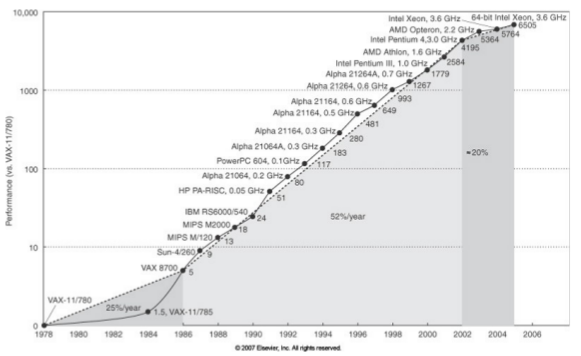
\includegraphics[height = 5cm, width = 7cm, keepaspectratio]{Moores.png}
\label{fig:moores}
\caption{Exemple de la Loi de Moores}
\end{figure}
\paragraph{Densité des processeurs}
\begin{itemize}
\item Intel 4004, 1971, 10000nm, .74MHz, 2300 transistors
\item Intel 8086, 1978, 3000nm, 8MHz, 29000 transistors
\item Intel 80386DX, 1985, 1000nm, 33MHz, 275000 transistors
\item Pentium Pro, 1995, 600nm, 150MHz, 5.5M transistors
\item Pentium 4, 2000, 180nm, 1.7GHz, 42M transistors
\item Intel Core 2, 2006, 65nm, 3.0GHz, 291M transistors
\item Xeon Westmere, 2012, 32nm, 2600M transistors
\item 15 cores Xeon Ivy Bridge EX, 2014, 22nm, 4310M transistors
\item 22 cores Xeon Broadwell, 2016, 14nm, 7200M transistors
\end{itemize}
\paragraph{Périphériques}
\begin{itemize}
\item Interface réseau: 1Gbit/s, 12\$;
\item Disque: 6TB, 750MB/s, \$150;
\item Mémoire non volatile: 1TB, 750MB/s, \$300;
\item Rubans: LTO-5, 3TB, \$2000;
\item Carte graphique: GP100 Pascal, 16nm, 15300M
transistors, 3584 coeurs;
\end{itemize}
\paragraph{Répertoire d'instructions}
\begin{itemize}
\item IBM 360
\item DEC VAX 11
\item Motorola 68000
\item Intel 80386
\item Sun SPARC
\item IBM PowerPC
\item ARM
\item Intel Itanium
\item Intel 64 (AMD64)
\end{itemize}
\paragraph{Classes d'ordinateurs}
On peut aussi classer les ordinateurs en différentes catégories, en voici un exemple.
\begin{itemize}
\item Super-ordinateur, entre 5 et 20M\$, grande pièce dédiée;
\item Serveur d'entreprise (mainframe), entre 1 et 5 M\$, coin de
pièce;
\item Serveur départemental, occupe un coin de pièce, entre
50K\$ et 1 M\$;
\item Poste de travail (workstation), dessus de bureau, 4K\$ à
50K\$;
\item Micro-ordinateur, dessus de bureau ou creux de la main,
100 à 4K\$;
\end{itemize}

À présent, la mode est dans le nuage et les grappes d'ordinateurs. c'est flexible, efficace avec virtualisation. Ça l'a un bon rapport performance prix avec une bonne dimension sur la consommation d'énergie. C'est un grand système parallèle en réseau. \\

Depuis quelques années, on a plafonnés en terme d'amélioration de vitesse par processeurs, alors on cherche à avoir quand même des gains de performances, mais au lieu d'améliorer la vitesse on parallélise notre travail sur plusieurs coeur différents. \\

Cela fait en sorte que la mémoire centrale et les disque n'augmentent pas de vitesse autant que le processeur.\\

On peut maintenant jouer aussi à des jeux 3D et du vidéo HD. On voit aussi la complexié des systèmes augmenter de manière exponentielle, ce qui à faire naître une panoplie d'outils de monitoring et vulnérabilités.

\paragraph{Historique des Systèmes parallèles}
\begin{itemize}
\item Burroughs D825, 1962, 4 processeurs;
\item Honeywell Multics System, 1969, 8 processors;
\item ILLIAC IV, 1965-1976, Vector machine, 256 units;
\item Cray 1, 1976, Vector machine;
\item Cray 2, 1985, 8 processors;
\item Multi-processeurs (SGI, SUN, IBM);
\item Grappes de calcul (Intel, IBM, HP...);
\end{itemize}

\paragraph{Programmation des systèmes parallèles.}
\begin{itemize}
\item FORTRAN, compilateurs parallélisants, HPF;
\item C, Parallel C, UPC, OpenMP (C et FORTRAN);
\item PVM, Linda, MPI;
\item CUDA, OpenCL
\end{itemize}

\paragraph{Hiérarchie de mémoire}
La mémoire dans les ordinateurs peuvent être organiser dans une forme de hiérarchie. Typiquement, les mémoires avec beaucoup de places sont beaucoup plus lentes. Versus les mémoires rapide ayant beaucoup moins de place. Dans cette hiérarchie, on considère les mémoires plus rapide en haut allant aux plus lentes (en bas).

\begin{itemize}
\item Registres
\item Cache L1
\item Cache L2
\item Cache L3
\item Cache $L_n$
\item Mémoire vive NUMA
\item *disque* SSD
\item disque magnétique
\end{itemize}

\paragraph{Addresse}
Normalement, on dépose une addresse en numéro de bloc et en adresse dans ce bloc. Le taux de succès est proportionel au nombre d'accès complétés au niveau le plus haut sans interaction avec le niveau inférieur. ? \\

On peut définir:
\begin{align}
T_{acces moyen} = T_{acces succes} + taux_{echec} * penalite_{echec}
\end{align}

\paragraph{Mémoire Cache}
.\\
\begin{itemize}
\item Blocs de 4 à 128 octets
\item Temps d'accès succès 1-4 cycles;
\item Pénalité d'échec 8-32 cycles (accès 6-10), (transfert 2-22);
\item Taux d'échec 1 à 20 pourcent;
\item Dimension 1K à 512K (Intel Core I5, 32K I et 32K D);
\item Correspondance directe, associative, par ensemble;
\item Remplacement aléatoire ou LRU;
\item Ecriture simultanée ou réécriture;
\end{itemize}


\paragraph{Mémoire Centrale}
\begin{itemize}
\item Pages de 4K, 2M ou 4M octets;
\item Temps d'accès succès 10-100 cycles;
\item Coût de l'échec 500000-6000000 cycles (quelques dizaines de
milisecondes);
\item Taux d'échec .00001\%-.001\%;
\item Table de pages à 1, 2 ou 3 niveaux, (associatif, remplacement LRU);
\item Conversion adresse logique à adresse physique par matériel avec
cache (TLB);
\item Chargement des pages par le système d'exploitation;
\item Une portion du système d'exploitation est toujours en mémoire centrale.
\end{itemize}
\paragraph{Système d'exploitation}
\begin{itemize}
\item Interface avec les périphériques (pilotes);
\item Interface avec les processus (appels systèmes);
\item Gestion de la mémoire (mémoire des processus, mémoire
virtuelle, tampons E/S);
\item Systèmes de fichiers;
\item Contrôle des accès;
\item Ordonnancement;
\item Gestion des interruptions.
\end{itemize}

\section{Taxonomie de Flynn}
\paragraph{SISD}
ordinateur conventionnel
\paragraph{SIMD}
ordinateur qui peut faire des opérations sur plusieurs donné. Parfois de manière conditionnel (ordinateur vectoriel, GPGPU)
\paragraph{MIMD}
multi-core, grappes.. etc.

\section{Parallélisme}
\begin{itemize}
\item La même opération sur des données différentes
\item Le même programme sur des données différentes
\item Différents programmes sur les mêmes données ou des données différentes
\end{itemize}
\section{Associativité}
La définition d'associativité est:\\

exemple: \\
Si on a un bloc de 512 avec une associativité de 4, sa veut dire qu'on a 4 blocs différents. alors 4 bloc de 128.
\section{Fiabilité et Statistiques}
on définit:
\paragraph{MTBF} Mean Time Between Failure. Temps moyens entre les pannes
\paragraph{MTTF} Mean Time to Failure. Temps jusquà une panne
\paragraph{MTTR} Mean Time to Repaire. Temps moyens pour réparer la panne
\paragraph{Fiabilité: F} $F = MTBF = MTTF + MTTR$
\paragraph{Disponibilité : D} $D = \frac{MTTF}{MTTF+MTTR}$
\paragraph{Déterminer taux de pannes, Failure in Time}$FIT = \frac{1}{MTTF}$ exprimer en \# de pannes par milliard d'heures. \\
Les taux de pannes s'additionnent si la probabilité de panne ne dépend pas de l'âge (accident aléatoire plutot que l'usure).
\subparagraph{Exemple} MTTF total pour 10 disques.
(MTTF = 1Mh), \\
1 contrôleur, (MTTF = 0.5Mh),\\
1 alimentation, (MTTF = 0.2Mh),\\
FIT = $\frac{1}{\frac{10}{1Mh} + \frac{1}{0.5Mh} + \frac{1}{0.2Mh}} = 58823 heures$

\paragraph{Probabilité}
\subparagraph{Probabilité que $P_1$ et $P_2$ se produisent (conjonction)} $P_1 * P_2$
\subparagraph{Probabilité que de cas disjoints se produisent} $P_1 + P_2$
\subparagraph{Probabilité que m ordinateurs sur n soient fonctionnels}
p est la probabilité qu'un ordi soit fonctionel\\
$\frac{n!}{m! *(n-m)!}*p^{m}*(1-p)^{n-m}$ \\
ou on peut prendre l'inverse, soit = 1-probabilité de tous défectueux = $1 - (1-p)^n$
voir exemple des examens précédents pour plus d'explications.

\section{Mesure de performances}
On utilise généralement ces mesure pour évaluer la performance des systèmes en parallèle:
\begin{itemize}
\item Temps écoulé
\item Temps d'Utilisation du CPU, Mémoire, ETC.
\item Rendement, résultats/Temps pour ressources.
\item Accélération A = $\frac{P_{amelioration}}{P_{\neg amelioration}}$
\end{itemize}
\paragraph{Accélération Partielle, Loi d'Amdahl} 
$A_t = \frac{1}{(1-f) + \frac{f}{Ap}}$\\
ou At est l'accélération partielle, f est la fraction parallélisable de l'élément et Ap est le nombre de coeur/le facteur d'accélération parfait.\\
\paragraph{Facteur d'accélération, S(p)}= $\frac{T_{sequentiel}}{T_{avec.n.processeur}}$

\paragraph{Efficacité E(p) = } $\frac{S(p)}{p}$
Si fraction parallélisable f accélérée de p, \\
$S(p) = \frac{1}{((1-f) + \frac{f}{p}}$ S(p) tend vers $\frac{1}{1-f}$ si p très grand.
\newpage

\section{Exercices}
\subsection{1.1}
\paragraph{Question}
Une application parallèle prend 4\% de son temps pour diviser le travail et 3\% pour
réconcilier les réponses. Quelle est l'accélération maximale obtenue sur 10, 50,
100 ou 1000 processeurs?
\paragraph{Réponse}
LOI D'AMDAHL\\
La partie sérielle prend .03 + .04 = .07. La fraction parallélisable est donc de 1.0 -
.07 = 0.93. Le temps d'exécution pour n processeurs est donc de .07 + 0.93 / n.\\
Pour n = 10, 50, 100, 1000, le temps (accélération) devient:
.163 (6.1), .0886 (11.3), .0793 (12.6), .07093 (14.1).

\subsection{1.2}
\paragraph{Question}
L'architecture Intel 64 décompose son adresse 64 bits en 16 bits inutilisés, 4 * 9
bits pour 4 niveaux de table de pages et 12 bits d'adresse dans la page. La cache
L1 fait 32KiO, a une associativité de 4 et contient des blocs de 64 octets. Montrez
l'organisation de la hiérarchie de mémoire et décrivez comment se fait l'accès à
une donnée dont l'adresse virtuelle est fournie.

\paragraph{Réponse}
L'adresse de 64 bits se décompose en: 16 inutilisés, 9, 9, 9, 9 (index 0, 1, 2, 3),
12 pour octet dans la page. Pour un accès, la cache de prétraduction d'adresse
contient 128 entrées de 36 bits d'étiquette vs adresse physique. Dans une bonne
proportion des cas on y trouve l'adresse physique correspondant à l'adresse
logique cherchée.\\

Autrement, la table de page de niveau 0 est indexée avec le premier 9 bits,
menant vers une page de la table de niveau 1, indexée avec le second champ de
9 bits... jusqu'au niveau 3. Ce dernier niveau contient l'adresse physique et des
bits de statut (valide, accessible...).\\

Une fois l'adresse physique obtenue, il faut vérifier si elle se trouve en cache L1.
La cache de donnée de 32KiO contient 512 blocs de 64 octets et donc 128
ensembles de 4 blocs. On retrouve donc pour l'adresse de 64 bits: 16 inutilisés,
35 étiquette, 7 ensemble, 6 octet du bloc. Pour chaque ensemble, on a 4 blocs
avec leur étiquette correspondante dans la cache. Le numéro d'ensemble est
pris dans l'adresse et l'étiquette vérifiée avec celle des 4 blocs disponibles dans
l'ensemble pour voir si le bloc cherché est en cache. Autrement, il faut charger le
bloc contenant l'adresse physique recherchée à partir de la mémoire centrale (ou
d'une cache L2) vers la mémoire cache L1.
\subsection{1.3}
\paragraph{Question}
Un disque contient 4 plateaux de données avec des pistes de 2 à 4.4 cm du
centre. Les pistes sont distantes de .05 um et la densité de bits le long de chaque
piste est de 400000 bits par cm. Quelle est la capacité de ce disque? Son taux de
transfert maximal s'il tourne à 7200RPM?
\paragraph{Réponse}
Le rayon moyen des pistes est de :\\
$\frac{4.4+2}{2} = 3.2cm.$ \\
La piste moyenne contient:\\
$2 \pi * 3.2cm * 400000 b/cm = 8042477 bits/piste$\\
L'étendue est de:\\
$(4.4 -2) = 2.4cm.$ Il y a donc $2.4cm * 10000um/cm / .05um = 480000 pistes.$\\

Ceci donne un total de\\

 $8042477 pistes/plateau * 480000 bits/piste * 4
plateaux/disque / 8 bits/octet = 1.93 TeraOctets/disque.$\\

Le taux de transfert maximal est en piste 0, au rayon = 4.4cm. Nous avons\\

$2 \pi *
4.4cm * 400000 bits/cm * 4 plateaux / 8 bits/octet = 5529203 octets$ \\
dans ces pistes. \\
A 7200 RPM ou 7200/60 = 120 tours par seconde, cela donne 5529203
octets / tour * 120 tours/s = 663 MO/s.
\subsection{1.4}
\paragraph{Question}
Votre programme effectue un appel à fgets pour lire des données du disque.
Décrivez le traitement fait par la librairie et le système d'exploitation?
\paragraph{Réponse}
Premièrement, la librairie vérifie s'il reste des donnée dans le tampon de lecture
pour ce pointeur de fichier. Autrement, un appel système read est effectué. Le
système d'exploitation vérifie si le bloc désiré est dans ses tampons d'E/S et
sinon envoie une requête au contrôleur de disque et met le processus en attente.
Le contrôleur lit le bloc voulu, le copie en mémoire par DMA et envoie une
interruption au système d'exploitation. Le système d'exploitation change le statut
du processus à prêt et pourrait le relancer immédiatement.
\subsection{1.5}
\paragraph{Question}
On vous demande de mesurer la taille des blocs de cache L1 ainsi que la taille de
la cache L1. Comment feriez-vous?
\paragraph{Réponse}
Un vecteur peut être accédé en boucle déroulée pour différentes tailles de
vecteur. Lorsque la taille dépasse la grosseur de la cache L1 de donnée, le
temps d'accès moyen augmente rapidement. Ensuite, on peut lire dans un
vecteur de taille supérieure à L1 des octets consécutifs, 1 sur 2, 1 sur 3... Le
temps d'accès moyen augmente jusqu'à ce qu'on atteigne 1 sur taille du bloc.
\subsection{1.6}
\paragraph{Question}
Un additionneur 1 bit peut produire une somme sur 1 bit en une unité de temps
avec 6 portes logiques. Un additionneur 32 bits peut produire une somme de 32
bits avec 320 portes logiques en 6 unités de temps. Calculez le rendement de
chacun (travail / (matériel * temps))?
\paragraph{Réponse}
Somme 32 bits en 32t avec 6 portes: 1 / (32 * 6) = .0052\\
Somme 32 bits en 6t avec 320 portes: 1 / (6 * 320) = .00052
\subsection{1.7}
\paragraph{Question}
Chaque processeur dans un circuit multi-coeur peut exécuter 2G
Instructions/seconde avec un taux de succès en mémoire cache de 99.9\%, pour
des blocs de 64 octets. Quelle est la bande passante requise vers la mémoire
pour chaque processeur pour les instructions? Pour 100 processeurs? Un
système multi-coeur contient 100 de ces processeurs dans une grille 10x10 avec
3 canaux à 2GO/s partagés par colonne. Le contrôleur de mémoire centralisé peut
supporter 50GO/s. Est-ce que cette organisation peut soutenir le volume d'accès
mémoire requis pour les fautes de cache d'instructions des 100 processeurs?
\paragraph{Réponse}
2G Instructions/seconde avec un taux de succès 99.9\%, blocs de 64 octets, 100
processeurs, 3 canaux à 2GO/s partagés par colonne, contrôleur de mémoire
50GB/s. Ceci donne 2G lectures/s * (1-.999) * 64 octets = 128MO/s ou 1.28GO/s
par colonne et 12.8GO/s pour 100 processeurs.
\subsection{1.8}
\paragraph{Question}
Donnez un exemple de décomposition pour a) une même opération sur des
données différentes, b) un même programme sur des données différentes, c)
différents programmes sur les mêmes données ou des données différentes?
\paragraph{Réponse}
Nous pouvons avoir a) un calcul de seuil sur chaque pixel d'une image, b) un
calcul de rendu d'image sur différentes scènes d'un film, et c) différents
encodages vidéo sur un même film.
\subsection{1.9}
\paragraph{Question}
Votre serveur départemental alimente un laboratoire avec 24 ordinateurs (D=.99)
pour 20 équipes. Le serveur est en fait une machine virtuelle qui peut rouler sur
l'une ou l'autre de deux machines physiques (D=.999) redondantes, connectées
chacune à deux SAN (D=.999) partagés en mirroir. Chaque SAN est composé de
4 disques (D=.99) en RAID 5. Tout ceci est connecté par un réseau (D=.99999)
Quelles sont les chances pour au moins une équipe de ne pouvoir travailler? Quel
serait l'effet de la fiabilité du logiciel?
\paragraph{Réponse}.\\

Server : avoir deux défectueur, $0.001*0.001 = 1*10^{-6}$\\

\text{avoir n/24 serveur fonctionels,}\\

$\frac{24!}{n! * (24-n)!} * 0.99^{n} * 0.01^{24-n} $*voir formule*\\

$\Sigma_{n=20}^{24} = 0.999996373$\\

\text{avoir n/4 disque fonctionels},\\

$\Sigma_{n=3}^4 \frac{4!}{n!*(4-n)!} * 0.99^n * 0.01^{4-n}$\\

\text{SAN: deux défectueux, }$(1-(0.999*0.9994))^2 = 0.000002558$\\

\text{Réseau défectueux, }0.00001\\

\text{Prob que tout fonctionne} $(1-P_{serveur2defectueux}) * P_{+de20ordi} * (1-P_{SAN2defectueux}) * (1-P_{reseaux}) = 0.999982815$

\subsection{1.10}
\paragraph{Question}
Un problème de grande taille s'exécute en 24h sur un noeud et en 1h sur un
ordinateur parallèle de 16 noeuds identiques au premier. Quelle est la fraction
parallélisable du programme? Comment expliquez-vous de tels chiffres?
\paragraph{Réponse}
Le problème décomposé entre plus facilement en mémoire centrale ou en
mémoire cache et le tout s'exécute plus efficacement, présentant une
accélération plus importante que la réduction du problème. Non, la fraction
parallélisable n'est pas négative :-).
\chapter{Pthread et TBB}
\section{Fils d'exécution}
Le principe d'avoir des fils d'exécution est de pouvoir continuer le traitement avec un fil lorsqu'un fil est bloqué. Le processus conventionel est d'avoir une mémoire séparés avec une mémoire partagée optionel.
\begin{figure}[!ht]
\centering
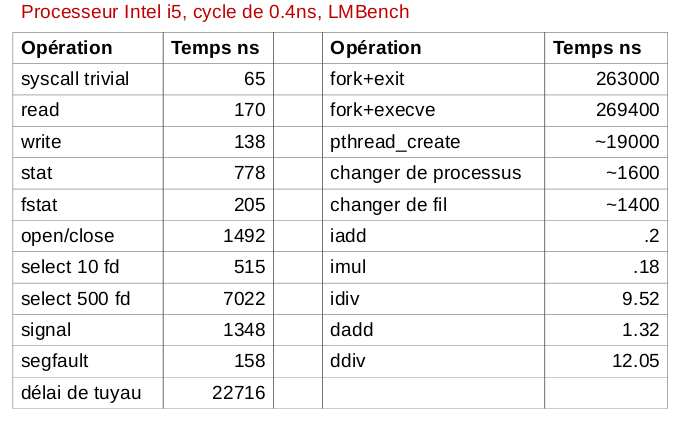
\includegraphics[width = 7cm, height = 5cm, keepaspectratio]{i5costs.png}
\caption{Les couts en termes de temps de processeurs pour certaines opérations de gestion de threads}
\label{fig:i5costs}
\end{figure}
\section{HyperThread}
La technologie hyperthread est en fait une grosse agace. Elle laisse croire qu'elle double la performance de ton processeur en ayant deux *core* par coeur physique de ton processeur. Cependant, c'est faux. \\

La technologie hyperthreading est en fait deux ensemble de registres pour un même processeur. Elle apparait comme deux processeur sauf que la performance n'augmente pas d'un facteur 2, elle augment d'environ 20 à 30 \%. \\

Lorsqu'un des processeur virtuel bloque sur un faute de cache ou quelque chose d'autre. l'autre coeur physique prend la place en un temps très mince et continuer d'exécuter. Cela fait en sorte que sa peut nuire au application parallèle et aux stratégies d'optimisation.
\section{Fils d'exécution en mode usager}
La création d'un fils d'exécution comporte les étape suivantes:
\begin{itemize}
\item Allouer de la mémoire sur la pile
\item inséré une entrée dans la tables de fils d'exécution.
\item créer un context qui pointe vers la pile
\end{itemize}
La fin d'un fil d'exécution : 
\begin{itemize}
\item Retirer l'entré dans la table des fils d'exécution
\item désallouer la pile et le contexte ou les conserver pour recyclage.
\end{itemize}
Yield: sauver le contexte courant (setjmp), changer pour le contexte d'une autre tâche (longjmp)

\section{Processus régulier (PThread)}
Le principe est que chaque processus peut se clôner a l'aide de l'appel système fork. en le clônant, on spécifie ce que le processus doit faire à l'aide d'une fonction qu'on rajoute dans sa pile. Le processus courant continue en même temps que le processus enfant et éventuellement attend le retour de l'enfant avec un waitpid. Le processus enfant démarre sa fonction à l'aide de la commande système exec en allouant des zones de mémoire partagée (si il a besoin de communiquer avec le processus parent). L'enfant à lui-même le contenue initial de mémoire virtuelle avec une copie des descripteurs de fichiers. l'enfant n'hérite pas des signaux, temporisateurs, verrous.. Il doit l'avoir à partir des données qui lui sont passer par son processus parent. \\
\subsection{Commandes}
\paragraph{Création}pthread\_create(\&tid,..);
\paragraph{Le parent attend souvent après l'enfant:} pthread\_join(tid, ...);\\
l'enfant partage la mémoire et toutes les ressources avec le parent mais utilise une partie différente de leur mémoire pour sa pile (une pile dans une pile).\\

\paragraph{avantages}
\begin{itemize}
\item Même espace mémoire et table de page pour les fils d'exécution d'un même processus = plus compact, création et changement de contexte plus rapides
\item Plus de coeurs physique = beaucoup plus de performance.
\end{itemize}
\paragraph{désavantages}
\begin{itemize}
\item Taille moins flexible pour les piles;
\item Tout usage concurrent de données partagées doit être protégé par des verrous ou accédé avec des opérations atomiques.
\item Réentrance: une interruption peut survenir n'importe quand, l'ordre des données n'est pas nécessairement le même.. gros shitshow.
\item Concurrence: On peut avoir deux ou plusieurs thread qui veulent accéder aux mêmes données en même temps.
\end{itemize}

\section{Pthread}
Le principe de pthread, comme le principe générale de la programmation parallèle, est de séparer le travail en plusieurs parties et de se servir des différents coeur de notre ordinateur pour pouvoir accomplir ce travail.\\
De cette manière, le travail pourra quand même continuer si on a des erreurs de bloquage d'E/S (fautes de caches). Pour ce, on devra simplifier le travail de manière asynchrone, avoir un gestionnaire qui aliment un bassin de travailleurs (un thread pool). On divisera le travail de différentes manière. On peut y aller de façon hiérarchique, avec une pipeline, des groupes de pairs, etc.
\subsection{Fonctions}
\begin{itemize}
\item \textbf{pthread\_create(thread,attr,start\_routine,arg)}\\
Cette fonction créer un thread et l'exécute, elle à comme argument:\\

thread : c'est le thread, on l'initialise au début du programme quand on fait notre thread pool \\

attr : l'attribut de cet thread, on peut changer toute sorte de chose comme la grosseur de la pile, certaines charactéristique qui y sont essentiels pour l'ordonnanceur. \\

start\_routine : la fonction que nous allons exécuter sur ce thread, souvent appeller *worker* ou quelques chose de similaire \\

arg: les argument que nous allons passer à notre thread. C'est obliger d'être un pointeur à un void. Normalement, on initialise une forme de structure, on la sérialise avec le pointeur en la passant à la thread, et ensuite à l'intérieur de la fonction on applique un cast de la forme de la structure originale pour qu'elle reprenne ses champs et soit accessible.\\

\item \textbf{pthread\_exit(status)}\\

Fonction qui sert à sortir de la thread, on se sert de la variable status pour envoyer un message à notre processus parent si nécessaire.\\

\item \textbf{pthread \_cancel(thread)}\\

On ferme notre thread, on se sert de cette fonction si on à besoin de fermer nos thread sans vraiment avoir besoin de rien en retour.\\

\item \textbf{pthread\_attr\_init(attr)}\\

Cette fonction sert à faire l'initialisation des attributs de nos threads, c'est essentiel à l'ordonnanceur, sauf que sa marche sans mettre de valeurs (les valeurs par défaut sont bonnes)\\
\item \textbf{pthread\_join(threadid, status)}\\

Cette fonction sert à joindre nos threads enfant au thread parents, normalement, elle sont appellés par les thread parents et l'appel de cette fonction fait attendre la thread parent jusqu'à temps que la thread enfant finisse la fonction start\_routine ou que celle-ci fait appel à \textbf{pthread\_exit()}.\\

\item \textbf{pthread\_detach(threadid)}\\
On utilise cette fonction si on veut défaire le lien entre un thread paren et un thread enfant, pour des cas très spécifiques.\\

\item \textbf{pthread\_attr\_setstacksize(attr, stacksize)}\\
On utilise cette fonction pour spécifier une grandeur de notre piles.\\
\item \textbf{pthread\_mutex\_init(mutex, attr)}\\

Cette fonction sert à initaliser un mutex.\\

\item \textbf{pthread\_mutex\_destroy(mutex)}\\

Sert à détruire un mutex.\\

\item \textbf{mutex\_attr\_..... init ou destroy(attr)}\\

Fonctions qui sert à initialiser ou à détruire des attribut de mutex.

\item \textbf{pthread\_mutex\_lock...unlock..trylock(mutex)}\\

Fonctions qui sert à barrer un mutex, le débarrer, ou essayer de le débarrer. Faut faire attention à l'ordre de verrouillage sinon on peut sa ramasser dans un deadlock.

\item \textbf{pthread\_cond\_init(condition, attr)}\\

Initialise une condition pour notre thread.

\item \textbf{pthread\_cond\_destroy(conditon)}\\

Détruit..

\item \textbf{pthread\_condattr\_init...destroy()}\\

...

\item \textbf{pthread\_cond\_wait(condition, mutex)}\\

Attend jusqu'à une certaines conditions pour un mutex ??

\item \textbf{pthread\_cond\_broadcast(condition)}\\

..
\end{itemize}

\subsection{Exemples Pthreads}

\begin{lstlisting}[language=C]
// exemple_pthreads.c
#define _REENTRANT
#include <pthread.h>
#include <unistd.h>
#include <stdio.h>
void afficher(int n, char lettre){
	int i,j;
	for (j=1; j<n; j++){
		for (i=1; i < 10000000; i++);
		printf("%c",lettre);
		fflush(stdout);
	}
}
void *threadA(void *inutilise){
	afficher(100,'A');
	printf("\n Fin du thread A\n");
	fflush(stdout);
	pthread_exit(NULL);
}

void *threadC(void *inutilise){
	afficher(150,'C');
	printf("\n Fin du thread C\n");
	fflush(stdout);
	pthread_exit(NULL);
}

void *threadB(void *inutilise){
	pthread_t thC;
	pthread_create(&thC, NULL, threadC,NULL);
	afficher(100,'B');
	printf("\n Le thread B attend la fin du thread C\n");
	pthread_join(thC,NULL);
	printf("\n Fin du thread B\n");
	fflush(stdout);
	pthread_exit(NULL);
}

int main(){
	int i;
	pthread_t thA, thB;
	printf("Creation du thread A");
	pthread_create(&thA, NULL, threadA, NULL);
	pthread_create(&thB, NULL, threadB, NULL);
	sleep(1);
	//attendre la fin des threads
	printf("Le thread principal attend que les autres se terminent\n");
	pthread_join(thA,NULL);
	pthread_join(thB,NULL);
	exit(0);
}
\end{lstlisting}
Cette exemple donne comme sortie : \\

-bash-3.2\$ ./exemple\_threads
Creation du thread
AACBACBACBACBACBACBACBACBACBABCABCABCABCABCABCABCA
BCABCABCABCABCABCABCABCACBACBACBACBLe thread principal
attend que les autres se terminent
ACBACBACBACBACBACBACBACBACBACBACBACBACBACBACBACBAC
BACBACBACBACBACBACBACBACBACBACBACBACBACBACBACBACBA
CBACBACBACBACBACBACBACBACBACBACBACBACBACBACBACBACB
ACBACBACBACBACBACBACBACBACBACBACBACBACBACBACBACBAC
BACBACBACBA
Fin du thread A
CB
Le thread B attend la fin du thread C
CCCCCCCCCCCCCCCCCCCCCCCCCCCCCCCCCCCCCCCCCCCCCCCCCC
Fin du thread C
Fin du thread B
-bash-3.2\$

\paragraph{Exemple du TP1}
Voici un autre exemple de pThread. Cet exemple est tirer du TP1.

\begin{lstlisting}[language=C]
/*
 * dragon_pthread.c
 *
 *  Created on: 2011-08-17
 *      Author: Francis Giraldeau <francis.giraldeau@gmail.com>
 */

#define _GNU_SOURCE
#define stacksize 2097152 // on donne une grosseur de 2 Mb pour notre stack, sa devrait etre suffisant
#include <stdlib.h>
#include <pthread.h>
#include <stdarg.h>
#include <string.h>

#include "dragon.h"
#include "color.h"
#include <sys/types.h>
#include <sys/syscall.h>
#include <unistd.h>
#include "dragon_pthread.h"
int gettid(void);
pthread_mutex_t mutex_stdout;



void *dragon_draw_worker(void *data){
  /* on initialise nos variable, code_erreur est evident,
   tdat sont nos donnes pour chaque 
	 threads, *canvas sont now points de depart pour
	  l'initialisation de la surface. On doit 
	 utiliser des differents points de depart vu que le
	  range n'est pas le meme que notre start et
	 end habituel  */
  int code_erreur;
  struct draw_data* tdat = (struct draw_data *) data;
  int startcanvas = 
  (tdat->id)*((tdat->dragon_width * tdat->dragon_height)/tdat->nb_thread);
  int endcanvas = 
  (tdat->id + 1) * ((tdat->dragon_width*tdat->dragon_height)/tdat->nb_thread);
  int start = (tdat->id)*(tdat->size/tdat->nb_thread);
  int end = (tdat->id + 1) * (tdat->size / tdat->nb_thread);


  //cette ligne sert a debugger les
  // points de depart dans les differentes threads.
  //elle indique les points de depart de chaque threads dans le terminal
  
  //printf("start is %d, end is %d, i is %d\n",start, end, tdat->id);
  
	/* 1. Initialiser la surface */
  //on initialise avec nos variables dependamment du thread ou l'on se situe
  
  init_canvas(startcanvas, endcanvas, tdat->dragon, -1);
	/* 2. Dessiner le dragon */
  //on dessine avec nos variables

  //printf("nous sommes rendu au wait de la thread %d\n", tdat->id);
  code_erreur = pthread_barrier_wait(tdat->barrier);
  //printf("nous avons passer la barriere %d\n", tdat->id);

  if(code_erreur != -1 && 0){
    //error handling de la barriere, cependant selon les man
    // pages de barrier_wait, ne devrait jamais se produire
    printf("erreur dans la barriere %d, code %d\n",tdat->id, code_erreur);
  }

  
  dragon_draw_raw(start, end, tdat->dragon, tdat->dragon_width,
   tdat->dragon_height, tdat->limits, tdat->id);
  
	/* 3. Effectuer le rendu final */

  /**/
  
  
  
  return NULL;
}

int dragon_draw_pthread(char **canvas, struct rgb *image,
 int width, int height, uint64_t size, int nb_thread)
{
  //TODO("dragon_draw_pthread");

	pthread_t *threads = NULL;
	pthread_barrier_t barrier;
	pthread_attr_t Attr;
	limits_t lim;
	struct draw_data info;
	char *dragon = NULL;
	int i;
	int scale_x;
	int scale_y;
	struct draw_data *data = NULL;
	struct palette *palette = NULL;
	int ret = 0;
	void * status;
	int code_erreur;

	pthread_attr_init(&Attr);

	threads =  malloc(sizeof(pthread_t)* nb_thread);
	pthread_attr_setstacksize(&Attr, stacksize);
	pthread_attr_setdetachstate(&Attr, PTHREAD_CREATE_JOINABLE);

	data = malloc((sizeof(struct draw_data)) * (nb_thread+1));

	
	palette = init_palette(nb_thread);
	if (palette == NULL)
		goto err;

	/* 1. Initialiser barrier. */
	pthread_barrier_init(&barrier, NULL, nb_thread +1);
	

	if (dragon_limits_pthread(&lim, size, nb_thread) < 0)
		goto err;

	info.dragon_width = lim.maximums.x - lim.minimums.x;
	info.dragon_height = lim.maximums.y - lim.minimums.y;

	if ((dragon = (char *) malloc(info.dragon_width * info.dragon_height)) == NULL) {
		printf("malloc error dragon\n");
		goto err;
	}

	if ((data = malloc(sizeof(struct draw_data) * nb_thread)) == NULL) {
		printf("malloc error data\n");
		goto err;
	}

	if ((threads = malloc(sizeof(pthread_t) * nb_thread)) == NULL) {
		printf("malloc error threads\n");
		goto err;
	}

	info.image_height = height;
	info.image_width = width;
	scale_x = info.dragon_width / width + 1;
	scale_y = info.dragon_height / height + 1;
	info.scale = (scale_x > scale_y ? scale_x : scale_y);
	info.deltaJ = (info.scale * width - info.dragon_width) / 2;
	info.deltaI = (info.scale * height - info.dragon_height) / 2;
	info.nb_thread = nb_thread;
	info.dragon = dragon;
	info.image = image;
	info.size = size;
	info.limits = lim;
	info.barrier = &barrier;
	info.palette = palette;
	info.dragon = dragon;
	info.image = image;

	for(i = 0; i < nb_thread; i++){
	  data[i] = info;
	  data[i].id = i;
	}

	 \\ 2. Lancement du calcul parallele principal avec draw\_dragon_worker 

	for(i = 0; i< nb_thread; i++){
	  code_erreur = pthread_create(&threads[i], &Attr, dragon_draw_worker, 
	  (void *) &data[i]);
	  if(code_erreur){
		printf("erreur dans la creation de la thread %d dans draw_dragon_pthread,
		 code %d \n",i, code_erreur);
		goto err;
	  }
	}

	/* 3. Attendre la fin du traitement */
	//printf("nous sommes rendu au wait de la main\n");
	pthread_barrier_wait(&barrier);
	//printf("nous avons passer la barrier de la main \n");
	for(i = 0; i< nb_thread; i++){
	  code_erreur = pthread_join(threads[i], &status);
	  if(code_erreur){
		printf("erreur dans le join de la thread %d dans draw_dragon_pthread,
		 erreur code %d \n", i, code_erreur);
		goto err;
	  }
	}
	scale_dragon(0, height, image, width, height, dragon, info.dragon_width,
	 info.dragon_height, palette);
	/* 4. Destruction des variables (a completer). */

	/*la plupart des variable a detruire sont tous dans "done"
	, la seule exception etant status et info.
	 info genere une erreur de segmentation si on la detruit alors 
	  j'assume qu'elle est utiliser ailleur. */
	free(status);
	goto done;
done:
	FREE(data);
	FREE(threads);
	free_palette(palette);
	*canvas = dragon;
	return ret;

err:
	FREE(dragon);
	ret = -1;
	goto done;
}

void *dragon_limit_worker(void *data)
{
  struct limit_data *lim = (struct limit_data *) data;
  
  //cette ligne imprime le TID de la thread
  printf("tid of thread is %d\n",(int) gettid());
  
  piece_limit(lim->start, lim->end, &lim->piece);
  return NULL;
}

/*
 * Calcule les limites en terme de largeur et de hauteur de
 * la forme du dragon. Requis pour allouer la matrice de dessin.
 */
int dragon_limits_pthread(limits_t *limits, uint64_t size, int nb_thread)
{
	void * status;
	int ret = 0;
	int i;
	pthread_t *threads = NULL;
	pthread_attr_t ptAttr;
	pthread_attr_init(&ptAttr);	
	struct limit_data *thread_data;  
	piece_t master;
	int code_erreur;
	pthread_attr_setdetachstate(&ptAttr, PTHREAD_CREATE_JOINABLE);

	piece_init(&master);

	/* 1. ALlouer de l'espace pour threads et threads_data. */
	
	//on associe la valeur defini de stack a nos pthreads et on fait un malloc
	// avec le nombre de limit_data par nombre de threads
	
	pthread_attr_setstacksize(&ptAttr, stacksize);
	threads = malloc(sizeof(pthread_t)*(nb_thread));
	thread_data = malloc((sizeof(struct limit_data)) * (nb_thread));
	
	/* 2. Lancement du calcul en parallele avec dragon_limit_worker. */
	
	/*initialisation des donnees pour les 
	differentes thread, on divise les valeurs entre 
	 *start* et *end* par le nombre de threads que nous avons. 
	 start --------------------------------------------------------------------> end
	 Thread1 ----> Thread 2 ----> Thread 3 ----> ..... ------------------------> end*/
	
	for(i = 0; i < nb_thread ; i++){
	  thread_data[i].id = i;
	  thread_data[i].start = (int)(i)*(size/nb_thread);
	  thread_data[i].end = (int)(i+1)*(size/nb_thread);
	  thread_data[i].piece = master;


	  //cette ligne sert a debugger les differentes threads, veuillez enlever
	  // le comment pour voir les points de
	  //depart de chaque thread dans le terminal
	  
	  
	  printf("start is %d, end is %d, id of thread is %d\n",(int)thread_data[i].start, 
	  (int)thread_data[i].end, (int)thread_data[i].id);
	}
	// on creer nos threads avec dragon_limit_worker et nos differents points de depart
	for(i = 0; i < nb_thread ; i++){
	  code_erreur = pthread_create(&threads[i],&ptAttr, dragon_limit_worker,
	   (void *) &thread_data[i]);
	  if (code_erreur){
		printf("nous avons une erreur dans la thread %d",i);
		goto err;
	  }
	}
	//on join les threads lorsqu'ils ont finient 
	//le travaille et on merge les differents morceau.
	for(i = 0; i < nb_thread ; i++){
	  code_erreur = pthread_join(threads[i], &status);
	  if(code_erreur){
		printf("nous avons une erreur dans le join de la thread %d", i);
		goto err;
	  }
	  piece_merge(&master, thread_data[i].piece);
	}
	
	/* 3. Attendre la fin du traitement. */
	goto done;
done:
	FREE(threads);
	FREE(thread_data);
	*limits = master.limits;
	return ret;
err:
	ret = -1;
	goto done;
}


\end{lstlisting}
\newpage

\section{TBB}

TBB est une librairie qui cherche à accomplir les mêmes chose que pthreads. Par contre, il y a des différences fondamentales. \\

La librairie travaille à un plus haut niveau, c-à-d. en language c++. sa nous permet de décrire l'algorithme parallèle plutot que d'être obliger de gérer manuellement tous les threads. C'est souvent plus efficace étant donné que c'est des experts qui ont fait la librairie..\\

C'est indépendant de la plate-forme et fonctionne seulement sur les processeurs intel. C'est basé sur des templates et utilise une différente taxonomie (task au lieu de threads). \\

Le fonction de la librairie, en générale, est qu'on doit faire un overload de l'opérateur () comme méthode dans notre class. ensuite on applique la fonction de tbb sur notre object et il va directement appeller les opérateurs () avec son range à lui.\\

On sépare le fonctionnement de la librairie en différente *template* de parallélisation, soit:


\subsection{for} : parallel\_for\\
une boucle for quand même normale. Pour le fonctionnement, on définit un overload de notre opérateurs pour itérer à traver la fonction défini dans l'overload. \\

comme argument, il prend un intervall 1d ou 2d et un objet avec un constructeur par copie et un opérateur () pour appliquer l'opération.\\

exemple : 
\begin{lstlisting}[language=C++]
parallel_for(blocked_range<size_t>(0,n), MyClosure(a));
\end{lstlisting}
 ou MyClosure est mon objet.\\


l'object initial est pris, et il est copier n fois. ou n est le nombre de fois ou TBB juge comme nécessaire de faire. toutes les object sont appliquer sur n intervalles. \\

La décomposition se fait en arbre jusqu'à ce que l'intervalle soit assez petit. en voici un exemple.

\begin{lstlisting}[language=C++]
struct TrivialIntegerRange {
	int lower;
	int upper;
	bool empty() const { return lower==upper; }
	bool is_divisible() const { return upper>lower+1; }
	
	TrivialIntegerRange( TrivialIntegerRange& r, split ) {
		int m = (r.lower+r.upper)/2;
		lower = m;
		upper = r.upper;
		r.upper = m;
	}
};

struct Average {
	const float* input;
	float* output;
	void operator()( const blocked_range<int>& range ) const {
	for( int i=range.begin(); i!=range.end(); ++i )
		output[i] = (input[i-1]+input[i]+input[i+1])*(1/3.f);
	}	
};
// Entree [0..n] and Sortie [1..n-1].
void ParallelAverage( float* output, const float* input,
size_t n
) {
	Average avg;
	avg.input = input;
	avg.output = output;
	parallel_for( blocked_range<int>( 1, n ), avg );
}

\end{lstlisting}

Exemple du TP1:
\begin{lstlisting}[language=c++]
class DragonDraw 
{
	public:
		DragonDraw(struct draw_data* parData)
		{
			data = parData;
		}
		DragonDraw(const DragonDraw& d)
		{
			data = d.data;
		}
		void operator()(const blocked_range<uint64_t>& r) const
		{
			int indexStart = ((r.begin() *data->nb_thread)/data->size);
			int indexEnd = ((r.end() * data->nb_thread)/ data->size);
			if(indexStart != indexEnd)
			{
				int firstStart = r.begin();
				int firstEnd = (indexEnd * data->size / data->nb_thread);
				int secondEnd = r.end();
dragon_draw_raw(firstStart,firstEnd,data->dragon,
data->dragon_width, data->dragon_height,data->limits, indexStart);
dragon_draw_raw(firstEnd,secondEnd,data->dragon,
 data->dragon_width,data->dragon_height,data->limits, indexEnd);
			}
			else
dragon_draw_raw(r.begin(),r.end(),data->dragon, 
data->dragon_width,data->dragon_height,data->limits, indexStart);	
		}
		struct draw_data* data;
};


int dragon_draw_tbb(char **canvas, struct rgb *image, int width, int height, uint64_t size, int nb_thread)
{
	//TODO("dragon_draw_tbb");
	struct draw_data data;
	limits_t limits;
	char *dragon = NULL;
	int dragon_width;
	int dragon_height;
	int dragon_surface;
	int scale_x;
	int scale_y;
	int scale;
	int deltaJ;
	int deltaI;

	tid = new TidMap(nb_thread);
	

	struct palette *palette = init_palette(nb_thread);
	if (palette == NULL)
		return -1;

	task_scheduler_init init(nb_thread);

	/* 1. Calculer les limites du dragon */
	dragon_limits_tbb(&limits, size, nb_thread);	
	dragon_width =limits.maximums.x - limits.minimums.x;
	dragon_height = limits.maximums.y - limits.minimums.y;
	dragon_surface = dragon_width * dragon_height;
	scale_x = dragon_width / width + 1;
	scale_y = dragon_height / height + 1;
	scale = (scale_x > scale_y ? scale_x : scale_y);
	deltaJ = (scale * width - dragon_width) / 2;
	deltaI = (scale * height - dragon_height) / 2;
	

	dragon = (char *) malloc(dragon_surface);
	if (dragon == NULL) {
		free_palette(palette);
		*canvas = NULL;
		return -1;
	}

	data.nb_thread = nb_thread;
	data.dragon = dragon;
	data.image = image;
	data.size = size;
	data.image_height = height;
	data.image_width = width;
	data.dragon_width = dragon_width;
	data.dragon_height = dragon_height;
	data.limits = limits;
	data.scale = scale;
	data.deltaI = deltaI;
	data.deltaJ = deltaJ;
	data.palette = palette;

	/* 2. Initialiser la surface : DragonClear */
	DragonClear clear(-1, dragon);
	parallel_for(blocked_range<int>(0, dragon_surface), clear);

	/* 3. Dessiner le dragon : DragonDraw */
	DragonDraw draw(&data);
	parallel_for(blocked_range<uint64_t>(0, data.size), draw);

	/* 4. Effectuer le rendu final */
	DragonRender render(&data);
	parallel_for(blocked_range<int>(0, height), render);
	cout << "Thread TBB : ";
	tid->dump();
	cout << "Nombre d'intervalle TBB : " << nIntervalle << endl;
	delete tid;
	
	init.terminate();

	free_palette(palette);
	*canvas = dragon;
	return 0;
}
\end{lstlisting}

\subsection{réduction} : parallel\_reduce

On applique une opération de réduction sur notre structure.\\

Elle doit avoir comme argument un intervalle, un object avec un constructeur par division, un overload de l'opérateur () pour appliquer la méthode de réduction (join).\\

exemple:

\begin{lstlisting}[language=c++]
parallel_reduce( blocked_range<size_t>(0,n), MySum(a) );
\end{lstlisting}

La décomposition est récursive, c-à-d. jusqu'à temps que l'intervalle soit assez petit. \\

À chaque feuille de l'arbre l'opérateur () est appliquer sur un range de notre grand range global. La recomposition (join) va ensuite cumuler les résultats obtenues.

\begin{lstlisting}[language=c++]
struct Sum {
	float value;
	Sum() : value(0) {}
	Sum( Sum& s, split ) { value = 0; }
	void operator()( const blocked_range<float*>& r ) {
		float temp = value;
		for( float* a=r.begin(); a!=r.end(); ++a ) {
			temp += *a;
		}
		value = temp;
	}
	void join( Sum& rhs ) {value += rhs.value;}
};

float ParallelSum( float array[], size_t n ) {
	Sum total;
	parallel_reduce( blocked_range<float*>( array, array+n ),
	total );
	return total.value;
}
\end{lstlisting}

On a aussi l'exemple du TP1...

\begin{lstlisting}[language=c++]
class DragonLimits {
        public:
                DragonLimits ()
                {
                 	piece_init(&p);
                }
                DragonLimits (const DragonLimits& d, split)
                {
                        piece_init(&p);
                }
                void operator() (const blocked_range<int>& r)
                {
                        piece_limit(r.begin(), r.end(), &p);
                }
                void join (DragonLimits& j)
		{
                        piece_merge(&p, j.p);
                }
                piece_t& getPiece ()
                {
                        return p;
		}
                piece_t p;
};

int dragon_limits_tbb(limits_t *limits, uint64_t size, int nb_thread)
{
	//TODO("dragon_limits_tbb");
	DragonLimits limit;
	task_scheduler_init init(nb_thread);
	parallel_reduce(blocked_range<int>(0, size), limit);
	piece_t piece = limit.getPiece();
	*limits = piece.limits;
	init.terminate();
	return 0;
}
\end{lstlisting}

\subsection{Scan} : parallel\_scan\\

Une autre méthode qui ressemble beaucoup au parallel\_reduce, on a comme argument un intervalle, un object avec constructeur par division, un opérateur () pour scan initial ou final afin de calculer la réduction. On utilise aussi un reverse\_join pour propager la réduction et assign pour l'initialiser. Prendre note, le nom des méthodes est importants.\\

exemple: 
\begin{lstlisting}[language=c++]
parallel_scan( blocked_range<int>(0,n), MyScan(a, b));
\end{lstlisting}

Scan fait la même chose que reduce, sauf qu'il ne redonne pas juste la dernière valeur, mais l'ensemble. Pour un vecteur 0,1,2,3,4,5,6,7,8,9; reduce nous donnerait :\\
45.\\
tandis que scan:\\
0, 1, 3, 6, 10, 15, 21, 28, 36, 45. \\

C'est utile lorsque plusieurs processeurs sont disponible. En voici un exemple.\\

\begin{lstlisting}[language=c++]
class Body {
	T sum; T* const y; const T* const x;
	Body( T y_[], const T x_[] ) : sum(0), x(x_), y(y_) {}
	T get_sum() const {return sum;}
	template<typename Tag>
	void operator()( const blocked_range<int>& r, Tag ) {
		T temp = sum;
		for( int i=r.begin(); i<r.end(); ++i ) {
		temp = temp + x[i];
		if( Tag::is_final_scan() ) y[i] = temp;
	}
	sum = temp;
	}
	Body( Body& b, split ) : x(b.x), y(b.y), sum(0) {}
	void reverse_join( Body& a ) { sum = a.sum + sum;}
	void assign( Body& b ) {sum = b.sum;}
};
float DoParallelScan( T y[], const T x[], int n ) {
	Body body(y,x);
	parallel_scan( blocked_range<int>(0,n), body );
	return body.get_sum();
}
\end{lstlisting}
\subsection{Do} parallel\_do\\
Le parallel do est une instance plus générale de parallélisation. On itère à travers une liste de tâches dans un *feeder*. Notre objet aura besoin d'un constructeur et d'un opérateur () encore une fois.\\

exemple. 
\begin{lstlisting}[language=c++]
parallel_do( first, last, MyClosure );
\end{lstlisting}
En plus, c'est possible d'ajouter des éléments directement au feeder. Par contre, la liste est parcouru séquentiellement, sa limite la mise à l'échelle.\\

Exemple.
\begin{lstlisting}[language=c++]
class Body {
	Body() {};
	typedef Cell* argument_type;
	void operator()( Cell* c, tbb::parallel_do_feeder<Cell*>& feeder )
	const {
		c->update();
		c->ref_count = ArityOfOp[c->op];
		for( size_t k=0; k<c->successor.size(); ++k ) {
			Cell* successor = c->successor[k];
			if( 0 == --(successor->ref_count) ) {
				feeder.add( successor );
			}
		}
	}
};
void ParallelPreorderTraversal( const std::vector<Cell*>& root_set ){
	tbb::parallel_do(root_set.begin(), root_set.end(),Body());
}
\end{lstlisting}

\subsection{Pipeline}
parallel\_pipeline\\
Le principe de la pipeline c'est de pouvoir mettre une entrée, l'entré va passer dans un élément de la pipeline, ensuite la sortie du premier élément de la pipeline va aller dans l'entrée de la deuxième élément. ainsi de suite. Utilisé normalement pour faire des filtres.\\
\begin{lstlisting}[language=c++]
pipeline.add_filter(filter& f);

pipeline.run(size_t max_number_of_live_token);
\end{lstlisting}
Exemple. 
\begin{lstlisting}[language=c++]
float RootMeanSquare( float* first, float* last ) {
	float sum=0;
	parallel_pipeline(16,make_filter<void,float*>(filter::serial,
	[&](flow_control& fc)-> float*{
		if( first<last ) return first++;
		else {
			fc.stop();
		return NULL;
		}
	}) &
	make_filter<float*,float>(filter::parallel,
		[](float* p){return (*p)*(*p);}) &
	make_filter<float,void>(filter::serial,
		[&](float x) {sum+=x;})
	);
	return sqrt(sum);
}
\end{lstlisting}

\subsection{Sort} parallel\_sort\\

Très simple, les deux arguments sont des itérateurs avec accès direct avec une fonction de comparaison et d'échange.

Exemple.

\begin{lstlisting}[language=c++]
#include "tbb/parallel_sort.h"
#include <math.h>
using namespace tbb;
const int N = 100000;
float a[N];
float b[N];
void SortExample() {
	for( int i = 0; i < N; i++ ) {
	a[i] = sin((double)i);
	b[i] = cos((double)i);
	}
	parallel_sort(a, a + N);
	parallel_sort(b, b + N, std::greater<float>());
}
\end{lstlisting}

\subsection{Tâches}
On effectue des sections de données en parallèle. On met des task dans une class et TBB va travailler dessus jusqu'à temps qu'il y en ait plus.\\

Les algorithme parallèles se divisent le problèmes en tâches qui sont ordonnancés entre les fils/processeur. Il est aussi possible de spécifier directement les tâches à faire exécuter efficacement en parallèle. Châque fil exécute une tâche à la fois, sans préemption. Lorsqu'il a fini, il prend la prochain tâche crée par le même fil jusqu'à temps qu'il y en ait plus.. Il est aussi possible d'assigner des priorités. \\

exemple.
\begin{lstlisting}[language=c++]
#include "tbb/task_group.h"
using namespace tbb;
int Fib(int n) {
	if( n<2 ) {
		return n;
	} else {
		int x, y;
		task_group g;
		g.run([&]{x=Fib(n-1);}); // spawn a task
		g.run([&]{y=Fib(n-2);}); // spawn another task
		g.wait();
		return x+y;
	}
}
\end{lstlisting}

l'ordonnancement de tâches de manière asynchrone sur plusieurs fils brise la propagation des exceptions normalement fournis par le c++. Les exceptions TBB peuvent être propagés d'un fil à l'autre pour remonter au fil de la tâche parent qui a crée les autres tâches.\\

On peut faire une structure qui permet l'accès concurrent. Les queues permettent de séparer des tâches parallèles mais un pipeline explicite est souvent mieux optimisé.
\begin{lstlisting}[language=c++]
concurrent_hash_map<Key,T,HashCompare>
concurrent_queue<T>
concurrent_vector<T>
\end{lstlisting}
On peut ajouter des mutex et autres..
\section{Exercice}
\subsection{2.1}
\paragraph{Question}
Comment pourriez-vous évaluer ou mesurer la taille requise par un programme
pour sa pile?
\paragraph{Réponse}
Statiquement, on peut regarder l'arbre d'appel (non récursif, sans pointeur de
fonction) et la taille de pile prise par chaque fonction. Dynamiquement, on peut
lire le pointeur de pile de temps en temps. Il est aussi possible de mettre un
quota sur la pile et de le diminuer jusqu'à ce qu'il y ait un problème
\subsection{2.2}
\paragraph{Question}
Vous avez un vieil ordinateur ayant appartenu à votre grand-père qui ne contient
qu'un seul processeur et un seul disque. Vous voulez y effectuer la compilation
d'un gros logiciel (e.g. noyau Linux). La compilation de chaque fichier demande un
mélange de calcul et d'accès disque. Combien de fils d'exécution devriez-vous
demander à parallel make? Combien de fils d'exécution demanderiez-vous pour
un serveur Web?
\paragraph{Réponse}
L'idée est d'utiliser le CPU en parallèle avec le disque. L'un ou l'autre sera le
goûlot d'étranglement et donc au mieux, avec deux fils, si la charge est égale
CPU et disque, cela pourrait aller deux fois plus vite. Plus de fils ne feraient
qu'encomber l'ordonnanceur et la mémoire cache. Pour un serveur Web, les
attentes après le réseau et les clients sont importantes et il est donc intéressant
d'avoir de nombreux fils, assez pour éviter qu'ils soient tous pris en attente, non
disponibles pour servir des requêtes.
\subsection{2.3}
\paragraph{Question}
Deux fils d'exécution communiquent entre eux par un tuyau bi-directionnel. Le
premier lit du disque et envoie au second une certaine quantité de donnée puis se
met en attente de la réponse et l'écrit sur disque. Le second traite les données au
fur et à mesure de leur réception et envoie le résultat aussi au fur et à mesure.
Est-ce correct? Peut-on procéder autrement?
\paragraph{Réponse}
Le problème est que le premier ne lit rien avant la fin alors que le second écrit au
fur et à mesure. Ceci causera problème à moins que le tampon associé au tuyau
soit plus grand que la quantité de données à traiter. Le second bloquera
rapidement en écriture et ne pourra plus lire, ce qui bloquera aussi le premier en
écriture.
\subsection{2.4}
\paragraph{Question}
Un débogueur insère des points d'arrêt en remplaçant l'instruction cible par une
instruction d'interruption (INT3). Une fois cet emplacement atteint, le programme
est interrompu et le INT3 retiré. Pour poursuivre, le débogueur repart l'exécution
en mode une instruction à la fois, replace le INT3 et repart l'exécution en mode
normal. On vous demande de changer le débogueur pour fonctionner en mode
non-stop, multi-fils: un point d'arrêt peut ne cibler qu'un seul fil d'exécution.
Comment feriez-vous?
\paragraph{Réponse}
La difficulté serait d'enlever et remettre le INT3 alors que d'autres fils continuent
leur exécution et doivent ou non s'arrêter sur cette instruction. La solution est de
recopier et d'exécuter l'instruction remplacée par le INT3 ailleurs (out of line) et
de compenser pour sa position modifiée (e.g. saut relatif au compteur de
programme).
\chapter{Cohérence Mémoire}
\section{Cohérence de Cache}
Ce chapitre est beaucoup moins axés sur la programmation, et beaucoup plus sur l'architecture des ordinateurs.\\

Il y a beaucoup d'organisation possible pour représenté la manière dont un ordinateur voit sa mémoire. voici un exemple. 
\begin{figure}
\centering
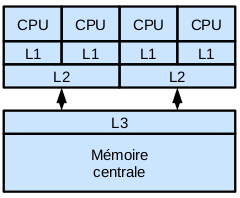
\includegraphics[height = 5cm, width = 7cm, keepaspectratio]{ArchitectureCache.png}
\caption{organisation de la mémoire cache dans un processeur multi-coeur}
\label{fig:architecturecache}
\end{figure}

Un aspect important est la Cohérence des caches, ce qui est un des points principale de ce chapitre.\\

Plusieurs scénario peut être possible. un processeur P1 écrit n dans X, lit X et trouve n. Par contre, un processeur P2 écrit n dans X, P1 lit x et peut trouver n si assez de temps est écoulé. Par contre, on ne peut jamais savoir combien de temps sa peut prendre. Les écriture sont propagées de manière asynchrone pour des fins de perfomances.\\

Normalement, pour une réécriture, la valeur est écrite en cache puis ensuite copiée ultérieurement en mémoire centrale. Par contre, il averti que le bloc a été modifié pour empêcher toute autre modification simultanée. Par contre, dans le cas d'un écriture immédiate, la valeur est immédiatement écrite en mémoire centrale, alors elle est visible par tous.\\

\begin{itemize}
\item \textbf{Cohérence par mise à jour}: une copie de la nouvelle valeur est envoyée à chaque copie en cache.
\item \textbf{Cohérence par invalidation}: avertir, lorsqu'un bloc est modifié, de détruire les copies maintenant invalides.
\item \textbf{status d'un bloc en cache}: Invalide, partagé (pour lecture seulement), exclusivité (peut petre écrit et lu).
\end{itemize}
Normalement, on a deux mode de cohérence de cache. Soit
\begin{itemize}
\item \textbf{MOESI}:\\
\begin{itemize}
\item Modified: Cette cache a la copie la plus récente, la seule, la copie en mémoire centrale est invalide.
\item Owned: cette cache a la copie la plus récente, d'autres peuvent avoir le status Shared, la copie en mémoire peut petre invalide.
\item Exclusive: cette cache a la copie la plus récente, la seul, la copie en mémoide est invalide (différence avec Modified)? peut-être que celle-ci peut seulement être modifié par elle?
\item Shared: Cette cache à la copie la plus récente, d'autres aussi, la copie en mémoire peut être invalide si une autre cache a la statut Owned.
\item Invalid: ce bloc ne peut être utilisé, son contenue n'est plus à jour.
\end{itemize}
\item \textbf{MESI}
\begin{itemize}
\item Modified: Cette cache a la copie la plus récente, la seule, la copie en mémoire centrale est invalide.
\item Exclusive: cette cache a la copie la plus récente, la seul, la copie en mémoide est invalide (différence avec Modified)? peut-être que celle-ci peut seulement être modifié par elle?
\item Shared: Cette cache à la copie la plus récente, d'autres aussi, la copie en mémoire peut être invalide si une autre cache a la statut Owned.
\item Invalid: ce bloc ne peut être utilisé, son contenue n'est plus à jour.
\end{itemize}
\end{itemize}
\paragraph{Cohérence par surveillance du bus} Était très populaire lors de l'âge des processeur avec peu de coeur, souvent avec des écriture simultanée. Le message de mise à jour ou invalidation est envoyé sur le bus, les autre cache incorporent cette information si elle contiennent le bloc visé dans leur cache.\\

L'accès au bus sérialise les accès.
\section{Cohérence par répertoire}
Pour chaque bloc, liste des processeurs qui en ont une copie avec un status modifié. \\
Lorsqu'un bloc est modifié, s'il était en mode partagé, le
répertoire est averti, un message d'invalitation est envoyé
aux autres copies et le statut devient modifié.\\

Pour accéder un bloc modifié, il faut prendre la nouvelle
copie et il devient partagé, non modifié. Le répertoire peut être réparti avec une fonction de
correspondance directe.
\paragraph{Surveillance versus répertoire}
La surveillance du bus est plus simple et était utilisé pour deux ou 4 processeurs, par contre, les processeurs actuels saturent trop rapidement le bus. La surveillance par Répertoire est plus compliqué mais requiert moins de communication.

\paragraph{l'architecture NUMA avec répertoire répartie}
Chaque processeur s'occupe d'une petite partie de la mémoire centrale et de son répertoire associé. voir fig \ref{fig:numa}.

\begin{figure}[!ht]
\centering
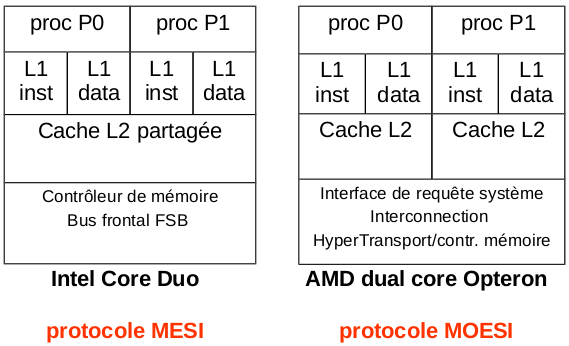
\includegraphics[height = 5cm, width = 7cm, keepaspectratio]{NUMA.png}
\caption{architecture NUMA sur les processeur intel et AMD.}
\label{fig:numa}
\end{figure}
Voici la configure de la génération AMD Bulldozer.

\begin{figure}[!ht]
\centering
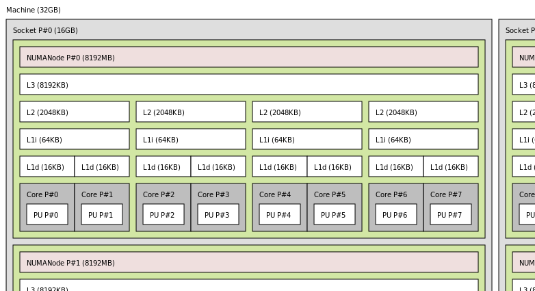
\includegraphics[height = 5cm, width=7cm, keepaspectratio]{AMDbulldozer.png}
\caption{AMD Bulldozer}
\label{fig:bulldozer}
\end{figure}

et voici l'architecture d'intel.. Skylake
\begin{figure}[!ht]
\centering
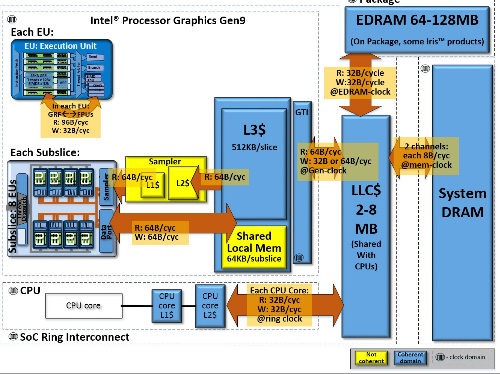
\includegraphics[height=5cm, width=7cm, keepaspectratio]{skylake.png}
\caption{configuration de la famille Skylake d'Intel}
\label{fig:skylake}
\end{figure}
Les i7 d'intels ont une TLB à chaque différent niveau de cache, en plus, ils ont une meilleur de faire des tabs qui leur permettent de garder leur memory mapping pour chaque différent processus.

\begin{figure}[!ht]
\centering
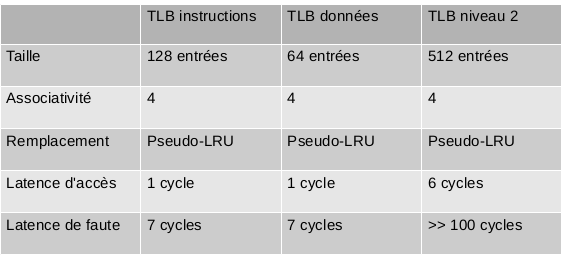
\includegraphics[height=5cm, width=7cm, keepaspectratio]{TLBi7.png}
\caption{TLB d'i7}
\label{fig:TLB}
\end{figure}

\begin{figure}[!ht]
\centering
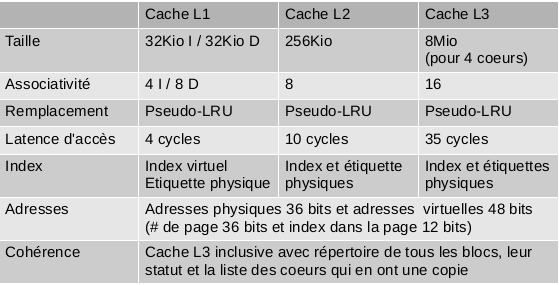
\includegraphics[height=5cm, width=7cm, keepaspectratio]{Cachei7.png}
\caption{Information sur les différent niveau de cache des i7}
\label{fig:Cachei7}
\end{figure}

\section{interface logiciel cache et TLB}
On a accès a un API qui nous permet de gérer le fonction de la TLB et de la cache, en voici des exemples.

\paragraph{TLB}
\begin{itemize}
\item void flush\_tlb\_all(void), quand la table de page du noyau change car elle est
reprise par tous les processus.
\item void flush\_tlb\_mm(struct mm\_struct *mm), quand tout l'espace d'un processus
change, lors d'un fork ou exec.
\item void flush\_tlb\_range(struct vm\_area\_struct *vma, unsigned long start, unsigned
long end), lorsqu'une partie d'espace d'un processus change, lors d'un munmap.
\item void flush\_tlb\_page(struct vm\_area\_struct *vma, unsigned long addr), lorsque
l'entrée pour une page change, suite à une faute de page.
\item void update\_mmu\_cache(struct vm\_area\_struct *vma, unsigned long address,
pte\_t *ptep), indique qu'une nouvelle entrée est disponible pour une page
virtuelle, par exemple pour précharger le TLB suite à une faute de page.
\item 
\end{itemize}
\paragraph{Cache}
\begin{itemize}
\item void flush\_cache\_mm(struct mm\_struct *mm), lorsque tout l'espace d'un processus
change, lors d'un exit ou exec.
\item void flush\_cache\_dup\_mm(struct mm\_struct *mm), lorsque tout l'espace d'un
processus change, lors d'un fork.
\item void flush\_cache\_range(struct vm\_area\_struct *vma, unsigned long start, unsigned
long end), lorsqu'une partie de l'espace d'un processus change, lors d'un munmap.
\item void flush\_cache\_page(struct vm\_area\_struct *vma, unsigned long addr, unsigned
long pfn), lorsqu'une page change, lors d'une faute de page.
\item void flush\_cache\_kmaps(void), lors d'un changement à highmem.
\item void flush\_cache\_vmap(unsigned long start, unsigned long end), et void
flush\_cache\_vunmap(unsigned long start, unsigned long end), lorsqu'une partie de
l'espace virtuel du noyau change, lors d'un map\_vm\_area ou unmap\_kernel\_range.
\item copy\_user\_page(...), copy\_to\_user\_page(...), clear\_user\_page(...), copy\_from\_user\_page(...), faire une
copie en tenant compte des problèmes d'alias (pour les dcache indexées virtuellement).
\item void flush\_dcache\_page(struct page *page), lorsque le noyau veut écrire ou lire une page qui peut aussi
exister dans l'espace virtuel d'un processus et faire un alias.
\item void flush\_anon\_page(struct vm\_area\_struct *vma, struct page *page, unsigned long vmaddr), avant que le
noyau accède une page anonyme qui pourrait être en alias.
\item void flush\_kernel\_dcache\_page(struct page *page), après que le noyau ait modifié une page qui peut être
en alias, pour enlever la copie de l'espace noyau en cache.
\item void flush\_icache\_range(unsigned long start, unsigned long end), lorsque du code exécutable vient d'être
écrit par le noyau car les caches instructions ne s'attendent normalement pas à du code modifiable.
\item void flush\_kernel\_vmap\_range(void *vaddr, int size), avant de faire une opération d'E/S sur une région en
mémoire, pour propager toute modification en mémoire centrale et enlever de la cache en vue de faire un
DMA.
\item void invalidate\_kernel\_vmap\_range(void *vaddr, int size), enlever de la cache avant de faire une lecture
d'E/S.
\end{itemize}
Les fautes de caches peuvent arriver pour plusieurs différentes raison.
\paragraph{Inévitable} La première accès cause toujours une faute de cache vue que le TLB n'est pas mapper sur le processus
\paragraph{Conflit} Si deux blocs chauds sont dans le même ensemble.
\paragraph{Capacité} Si le bloc requis a été évincé faute de place.
\paragraph{Contention} Si il y beaucoup de demande pour une écriture d'une variable.
\paragraph{Faux partage} Si jamais il y a deux variables qui sont modifiées par des processeurs différents et qui sont dans le même bloc de cache.

\section{Optimisation}
On peut optimiser en utilisant certaines modifications.

\paragraph{Pipelines superscalaires} Pipeline permettant d'exécuter plusieurs instructions en même temps et dans le désordre, tout en respectant les dépendances. sa se passe au niveau du processeur lui-même.\\

ex: deux instruction de add sur deux différent registre dans le même coup d'horloge.\\
\paragraph{Queues d'écritures}
\paragraph{Queus de message d'invalidations}
\paragraph{Bancs de mémoire cache qui peuvent être accédés en parallèle}

\paragraph{Explication de la pipeline superscalaire} Le compilateur optimiseur peut effectuer tout changement qui ne modifie pas le résultat final. Par exemple, il peut réordonnancer les écriture et lectures (faites dans des variables séparés ne présentant pas de dépendance). Les deux section sont équivalentes.
\begin{multicols}{2}

ld R1, A\\
ld R2, B\\
ld R3, C\\
... calcul ...\\
st R4, Resultat1\\
st R5, Resultat2\\

\columnbreak

ld R1, A\\
ld R3, C\\
ld R2, B\\
... calcul ...\\
st R5, Resultat2\\
st R4, Resultat1\\

\end{multicols}

Les écritures vers la mémoire cache peutventêtre mises en queue sans avoir d'attente synchrone.\\

Le contenue de la queue est consulté lors des accès en lecture pour assurer une cohérence entre cette écriture récente et une lecture qui suit sur le même CPU. Néanmoins, en mémoire centrale, les accès en écriture sont retardés (W$\rightarrow$R). Il peut y avoir plusieurs queues, en fait, un par banc de mémoire cache. Dans ce cas, l'ordre des écriture peut changer entre deux accès si une queu est plus pleine qu'une autre (W$\rightarrow$W).\\

\section{Contraintes d'ordonnancement}
\paragraph{Ordre séquentiel}: aucun réordonnancement. Toute ce fais dans l'ordre qu'il est écrit. Ne laisse pas place à beaucoup d'optimisation.

\paragraph{Ordre total des écriture (TSO)}: Les écriture peuvent être retardés par rapport aux lectures en raison des queues d'écriture. 

\paragraph{Ordre partiel des écritures(PSO)}: Les écriture à des variables différentes peuvent être retardés à des degrés divers (queus multiples).

\paragraph{Ordre faible(WO)}: les lecture peuvent être devancées (mises à jour retardées en queue d'invalidation) 

\section{Course entre deux processeur}
La cohérence entre le cache et le TLB est maintenue pour un processeur. Il doit n'y avoir qu'une seule copie maîtresse pour chaque bloc. Les mises à jours vers la copie maîtresse peuvent être retardés (queus d'écriture).\\

Les mises à jour vers les copies secondaires peuvent petre retardés (queues d'invalidations).\\

Le code suivant espère que p (next, key, data) sera écrit avant qu'il ne devienne accessible (head.next = p):

\begin{multicols}{2}
p$\rightarrow$next=head.next;\\
p$\rightarrow$key=key;\\
p$\rightarrow$data=data;\\

head.next = p;
\columnbreak
p = head.next;\\
while(p != \&head)\{\\
	if(p$\rightarrow$key==key)\{\\
		return(p);\\
	\}\\
	p = p$\rightarrow$next;\\
\}
\end{multicols}

Le compilateur et le pipeline peut réordonnancer les accès non dépendants.\\
Les queus d'écriture peut retarder et réordonnancer les écritures.\\
Les queue d'invalidation pourrait retarder la mise à jour de p et head (exemple d'en haut) même si head.next pointe déjà à p. (valeur non correct).

\section{forcer un réordonnancement}

On peut forcer un réordonnancement avec le API de linux. On utilise des instructions spéciales qui permet au compilateur de réordonnancer les accès (lecture, écriture ou les deux). On peut aussi le faire en mettant une  barrière dans le pipeline empêchant de réordonnancer les accès (lecture et écriture).\\

On peut aussi mettre une barrière dans les queues d'écriture pour retenir toutes les nouvelles écriture tant que celles avant la barrière ne sont pas terminées.\\

Finalement, on peut aussi mettre une barrière qui, lorsqu'une lecture arrive, bloque les accès le temps de traiter toutes les invalidations en queues.
\subsection{Instructions}
Noter que cmm n'est requis lorsqu'on est en mode utilisateur.
\begin{itemize}
\item barrier(): barrière pour le compilateur.
\item cmm\_smp\_rmb() en mode usager ou smp\_rmb() dans le noyau
Linux: barrière lecture pour le compilateur et le pipeline, et pour les
queues d'invalidation.

\item cmm\_smp\_read\_barrier\_depends(): barrière pour les queues
d'invalidation (les valeurs à synchroniser sont dépendantes et ne
seront pas touchées par le compilateur et le pipeline).

\item cmm\_smp\_wmb(): barrière d'écriture pour le compilateur et le
pipeline, et pour les queues d'écriture.
\item cmm\_smp\_mb(): barrière pour le compilateur, le pipeline, les
queues d'écriture et les queues d'invalidation.
\end{itemize}
\paragraph{Explications avec exemple}: Voir exemple en dessous \\

Une barrière cmm\_smp\_wmb() assure que p arrive en mémoire avant d'être accessible (head.next=p). Si p et head sont dans des blocs/bancs de cache différents, leur message d'invalidation peuvent être dans des queues différentes. Si la queue pour p est plus pleine, head peut arriver avant la mise à jour (invalidation) de p et l'ancienne valeur de p dans le cache du processeur 1 pourrait être lue, ce qui n'est pas bon du tout.\\

Une barrière cmm\_smp\_rmb() est trop conservatrice, cmm\_smp\_read\_barrier\_depends() est mieux. 
\begin{multicols}{2}
/* Processeur 0 */\\
p->next = head.next;\\
p->key = key;\\
p->data = data;\\
cmm\_smp\_wmb();\\
head.next = p;\\

\columnbreak

/* Processeur 1*/\\
p = head.next;\\
while (p != \&head) \{\\
/* ajouter barrière ici! */\\
if (p->key == key) \{\\
return (p);\\
\}\\
p = p->next;\\
\}\\
\end{multicols}
\section{Exercice}
\subsection{3.1}
\paragraph{Question}
Un multi-processeur à mémoire partagée adressable par mot (de 4 octets) vient
avec une mémoire cache associée à chacun des 4 processeurs. Cette mémoire
cache est à correspondance directe et contient 4 blocs de deux mots. Montrez le
statut de chaque bloc (MESI) après les accès suivants (processeur, P0 à P3, et
accès, R ou W suivi de l'adresse et valeur) si les caches sont initialement vides.
Discutez des communications dans les cas par mise à jour ou invalidation, et par
répertoire ou surveillance de bus.
\paragraph{Réponse}
P0: R 120; P0: W 120, 80; P3: W 120, 80; P1: R 110; P0: W 108, 48; P0: W 130,
78; P3: W 130, 78\\

Cache directe, 4 blocs de 2 mots, MESI\\
Adresse 32 bits: étiquette 29 / bloc 2 / mot 1\\
Adresses décomposées: 120: 15/0/0, 110: 13/3/0, 108: 13/2/0, 130: 16/1/0\\

Les blocs suivants sont touchés par les accès dans chaque cache. Lorsqu'un
bloc présent dans une autre cache (même étiquette) est accédé, il devient S. Si
le bloc écrit se retrouve dans une autre cache, il est invalidé dans l'autre cache et
modifié localement\\

P0: R 120, bloc 0 S; P0: W 120, 80, bloc 0 M; P3: W 120, 80, bloc 0 M, P0 bloc 0
I; P1: R 110, bloc 3 S; P0: W 108, 48, bloc 2 M; P0: W 130, 78, bloc 1 M; P3: W
130, 78, bloc 1 M, P0 bloc 1 I.
\subsection{3.2}
\paragraph{Question}
Un programme réinitialise un vecteur de 128 entiers de 4 octets à 0. Si la mémoire
cache associée au processeur contient des blocs de 64 octets, décrivez les
communications nécessaires sur le bus pour une cohérence par surveillance et
mise à jour versus par répertoire et invalidation.
\paragraph{Réponse}
Un programme réinitialise un vecteur de 128 entiers de 4 octets à 0, cache avec
blocs de 64 octets. Il y a donc 16 éléments entiers du vecteur dans chaque ligne
de cache. Avec surveillance et mise à jour, un message est envoyé sur le bus
pour chacun des 128 accès. Avec invalidation, une invalidation est envoyée à
chaque 16 accès au répertoire; si aucune autre cache ne contient le bloc, cette
invalidation n'est pas envoyée aux autres processeurs.
\subsection{3.2}
\paragraph{Question}
Deux variables mises à jour par des processeurs différents se retrouvent dans la
même ligne de cache. Ces variables servent à calculer une somme dans une
boucle et sont donc accédées une fois en lecture et une fois en écriture à chaque
fois (4 instructions à 1 cycle/instruction hormis les fautes de cache de 16 cycles de
pénalité). Comment peut-on se rendre compte d'un tel problème? Que peut-on
faire pour y remédier? Quel facteur d'amélioration pourrait en résulter?
\paragraph{Réponse}
Accès une fois en lecture et une fois en écriture à chaque fois (4 instructions à 1
cycle/instruction hormis les fautes de cache de 16 cycles de pénalité). Le
scénario probable est une faute de cache par tour de boucle pour 4+16=20
cycles versus 4 cycles. Un tel problème peut être détecté par des outils
spécifiques ou avec un bon outil de profilage des fautes de cache. Il suffit
d'aligner chaque variable sur une nouvelle ligne de cache pour y remédier.
\subsection{3.4}
\paragraph{Question}
Le processeur 0 exécute la fonction foo alors que le processeur 1 exécute la
fonction bar sur un ordinateur multi-processeur à mémoire partagée avec cache,
queues d'écriture et queues d'invalidation et le protocole de cohérence MOESI.
Les variables a et b sont globales et initialement à 0. Est-ce qu'il pourrait arriver
que l'assertion a==1 ne soit pas vérifiée? Expliquez?
\begin{lstlisting}[language=c]
void foo(void){ 
	a = 1;
	smp_wmb();
	b = 1;
}
void bar(void){ 
	while (b == 0) continue;
	assert(a == 1);
}

\end{lstlisting}
\paragraph{Réponse}
La barrière mémoire en écriture assure que b=1 arrivera après a=1 dans la copie
maîtresse de ce bloc de mémoire (en mémoire centrale ou en cache avec le
statut modified). Il faut toutefois s'assurer que les mises à jour (invalidations)
arrivent dans l'ordre sur le processeur 1, avec une barrière mémoire de lecture,
smp\_rmb(), entre les deux énoncés de la fonction bar.
\chapter{Modèle de mémoire partagée}
La programmation à mémoire partagée est un nouveau point de vue. Le compilateur optimiseur génère du code assembleur et peut changer la séquence si sa n'affecte pas le résultat. l'unité centrale de traitement peut changer la séquence des accès aussi en raison de ses tampons d'écriture et de son pipeline.\\

l'ordre des changements en mémoire vus par les différent processeurs peut différer\\

Si deux fils d'exécution communiquent par mémoire partagée, il ne peuvent nécessairement se fier sur l'ordre.. Jusqu'à date, ce sont des chose qui ont été mis au claire au chapitre 3.
\section{Modèle Partagé}
\paragraph{ Séquentiel}
Le processeur, lors d'exécution d'un modèle séquentiel, vois le travail dans l'ordre ou il est écrit. C'est à dire, toute le programme va être exécuter comme il est écrit. \\

Il attend qu'une écriture soit effective partout avant de continuer ou attend que les écriture de partout soit effective avant de continuer l'exécution du programme.\\

Cela fait en sorte que le modèle séquentiel est très contraignant, sa réduit donc beaucoup la performance. On peut relâchés différentes contraintes, ce qui nous fera utiliser des instructions de synchronisation pour s'assurer que le programme donne bien le résultats attendu.\\

Le modèle varie d'une architecture de processeur à un autre. Pour avoir le meilleur des deux mondes, nous devront utiliser des variables en mémoire partagé et utiliser des primitives de synchronisation pour s'assurer que tout soit cohérent.\\

Par contre, l'accès mémoire ne sera réordonnancé avec une écriture que si les deux sont à des cases mémoire différentes. Les accès simples et alignés sont atomique. Par contre, un accès double mot, ou non aligné pourrait être a moitié complété... Les opérations de synchronisation offertes par les librairies ou le système d'exploitation s'occupent de mettre les instructions requises pour qu'on puisse séquencer les opérations correctement.\\

Les lectures peuvent avoir lieu avant une écriture à une variable différente qui les précédait, contrainte W $\rightarrow$ R relâché (Total Store Order). \\

Les lecture et écriture à des variables différentes peuvent être réordonnancées par rapport aux écritutres containtes W $\rightarrow$R et W $\rightarrow$W relâchés (Partial Store Order).\\

Tous les accès à des variables différentes peuvent être réordonnancées (Weak Ordering).

\begin{figure}[!ht]
\centering
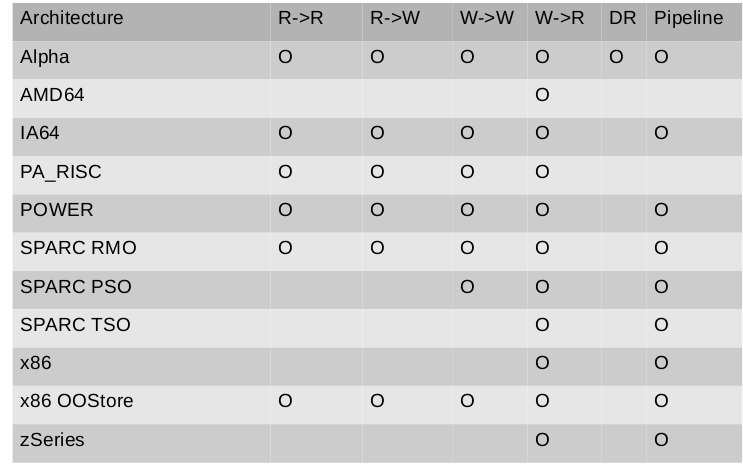
\includegraphics[width=7cm, height=5cm, keepaspectratio]{StoreOrder.png}
\caption{Exemple des différentes ordre de Storing}
\label{fig:StoreOrder}

\end{figure}
\newpage
Voici des éxemples:
\begin{multicols}{2}
Processeur 1\\

Flag1 = 1\\
if(Flag2 == 0) \{\\
*section critique*\\
\}\\

ou \\

Processeur 1\\
Data = 2000\\
Head = 1
\columnbreak

Processeur 2 \\

Flag2 = 1\\
if(Flag1 == 0)\{\\
*section critique*\\
\}\\

ou \\

Processeur 2\\
while(Head == 0)\{;\}\\
Value = Data\\

\end{multicols}
\subsection{Barrières}
On utilise les même barrières que dans la cohérence de cache. Soit:
\begin{itemize}
\item Barrière mémoire pleine: cmm\_smp\_mb() en mode usager ou smp\_mb() dans le
noyau Linux. Lectures ou écritures qui précèdent effectuées avant toutes les lectures
ou écritures qui suivent.

\item Barrière mémoire pour lecture: cmm\_smp\_rmb(). Lectures qui précèdent effectuées
avant les lectures qui suivent.

\item Barrière mémoire pour écriture: cmm\_smp\_wmb(). Ecritures qui précèdent
effectuées avant les écriture qui suivent.

\item Barrière mémoire pour lectures dépendantes: cmm\_smp\_read\_barrier\_depends().
Lectures qui précedent effectuées avant les lectures dépendantes qui suivent.

\item Barrière mémoire pour les E/S calquées sur la mémoire: mmiowb(). Correspond à un
nop dans la plupart des cas car jumelé à un spinlock qui vient avec les barrières
voulues.
\end{itemize}

\paragraph{Exemples:}

\begin{multicols}{2}
Processeur 1\\

Data = 2000\\
cmm\_smp\_wmb()\\
Head = 1\\

\columnbreak

Processeur 2\\

while(Head == 0) \{;\}\\
cmm\_smp\_rmb()\\
Value = Data\\
\end{multicols}

\begin{multicols}{2}
Processeur 1\\

a = 1\\
b = 2\\
cmm\_smp\_wmb()\\
c = 3\\
d = 4\\

\columnbreak

Processeur 2\\

v = c\\
w = d\\
cmm\_smp\_rmb()\\
x = a\\
y = b\\
\end{multicols}

\begin{figure}[!ht]
\centering
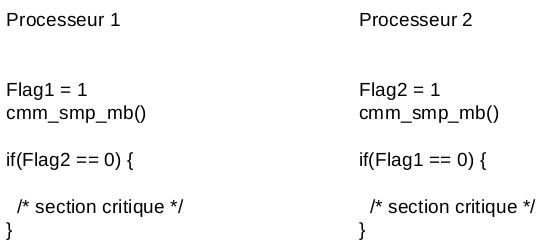
\includegraphics[height=5cm, width=7cm, keepaspectratio]{barrierememoire1.png}
\caption{exemple 1 barrière mémoire}
\label{fig:exemple1barriere}
\end{figure}

\begin{figure}[!ht]
\centering
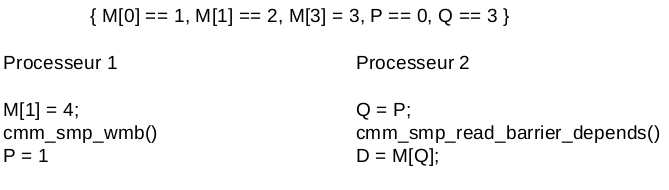
\includegraphics[height=5cm, width=7cm, keepaspectratio]{barrierememoire2.png}
\caption{exemple 2 barrière mémoire}
\label{fig:exemple2barriere}
\end{figure}

\paragraph{Architecture}
On a aussi certaine commande unique par architecture.
\begin{itemize}
\item X86: smp\_wmb() est nop, smp\_rmb() et smp\_mb() sont
réalisés avec lock,addl.
\item AMD64: smp\_rmb() est lfence, smp\_wmb() est sfence,
smp\_mb() est mfence.
\item PowerPC: smp\_rmb() est lwsync, smp\_wmb() et
smp\_mb() sont sync.
\item SPARC: smp\_rmb() est membar \#LoadLoad, smp\_wmb()
est membar \#StoreStore, smp\_mb() est membar
\end{itemize}

\paragraph{Vérifications}
Une barrière mémoire oublié ou un algorithme incomplent peut causer une course mémoire entre les différents processeurs. Il n'y a pas beaucoup de manière de débogger ce genre de problème (Tracer pendant des jours??). Il faut vraiment modéliser l'algorithme et le matériel pour le valider formellement en essayant toute les possibilités (model checking).\\

On a aussi accès à des mutex, comme:
\begin{itemize}
\item spinlock
\item mutex
\item semaphores
\item R/W semaphores
\item RCU
\end{itemize}
On prend et on redonne les mutex avec:\\

\paragraph{Lock} Les accès mémoire sont complétés après
\paragraph{Unlock} les accès mémoire avant seront complétés avant
\paragraph{Lock.. Unlock} Certaines opérations avant et après peuvent se mélaner à l'intérieur, ce n'est pas une barrière complètes..
\paragraph{Unlock.. Lock} barrière mémoire complète entre avant et après
\section{résumé}
Pour résumer la programmation en mémoire partagé, on suit les étapes suivantes:
\begin{enumerate}
\item Décomposer le travail en minisant les interactions (écriture dans des variables partagés entre les fil d'exécutions)
\item Synchroniser les accès aux variables partagées.
\item Lecture sans verrous, écriture atomique.
\item Verrou associé à une ou des variables.
\item Structure mises à jour par RCU.
\begin{itemize}
\item spinlock
\item R/W spinlock
\item mutex
\item semaphores
\item R/W semaphores
\item verrous usuels du RCU, par contre c'est très mauvais avec un grand nombre de processeurs
\end{itemize}
\item Protection des variables
\begin{itemize}
\item Processus avec signal, assurer néanmoins la réentrance pour les variables locales à un thread (CPU)
\item Section critique du noyau modifiant des variables et utilisant le CPUid: désactiver la préemption ou verrouiller. 
\item Dans le noyaus, désavticer les interruptions et désactiver la prééemption si aucun appel n'est fait qui puisse causer un réordonnancement.
\end{itemize}
\item Attendre que plusieurs fil d'exécution aient atteint un certain point
\item Join!
\end{enumerate}
\paragraph{Méthode de gestion de fils}
\begin{itemize}
\item Arbr: arbre de décomposition du problème, la racine attends après les enfants récursivement puis envoie le débloquage en sens inverse.

\item Papillon: chaque fil communique avec un autre à chaque étape (i+1\%n, i+2\%n, i+4\%n...) Tous reçoivent l'information que tous sont prèts en même temps, pas de phase d'annonce de fin! C'est le plus rapide, par contre il envoit beaucoup plus de message que les autres.
\end{itemize}
\section{Exercices}
\subsection{4.1}
\paragraph{Question}
Expliquez par quel mécanismes possiblement présents sur des architectures
modernes, les différentes contraintes W->R, W->W, R->R et R->W pourraient être
relâchées afin de gagner en performance?
\paragraph{Réponse}
Les queues d'écriture vont souvent retarder les écritures par rapport aux
lectures. Deux blocs de mémoire peuvent opérer en parallèle avec chacun leur
queue d'écriture et queue d'invalidation, et causer des réordonnancements
écriture écriture ou toute autre combinaison.
\subsection{4.2}
\paragraph{Question}
En quoi diffèrent les opérations de synchronisation comme les opérations
atomiques sur un mono-processeur versus sur un multi-processeur? Lequel est
plus coûteux?
\paragraph{Réponse}
Sur mono-processeur, il suffit de se prémunir contre la préemption, ce qui est en
général beaucoup plus court. Sur multi-processeur, un mécanisme est requis
pour assurer que la nouvelle valeur soit disponible et modifiée par le processeur
qui exécute l'opération atomique, sans interaction possible avec les autres
processeurs, un peu comme pour les barrières mémoire.
\subsection{4.3}
\paragraph{Question}
On veut remplacer l'allocateur de mémoire d'un système d'exploitation multi-
processeur par un allocateur qui maintient de la mémoire par processeur et la
plupart du temps peut servir les allocations localement sur le processeur.
Comment peut-on maintenir des structures “par processeur” en mémoire
partagée? Comment changent les besoins en synchronisation dans ce cas?
\paragraph{Réponse}
On peut avoir des structures par processeur soit en utilisant le numéro de
processeur comme indice dans un vecteur, ou en utilisant un registre. Il faut
toutefois se prémunir contre la préemption ou la migration de processeur.

\subsection{4.4}
\paragraph{Question}
Deux processeurs effectuent les opérations suivantes dans un système avec
ordonnancement faible. Quels sont les combinaisons de valeurs possibles à la fin?\\

Processeur 1:\\
A = 3;\\
B=4\\
Processeur 2:\\
x = A\\
y = B\\
\paragraph{Réponse}
permutation de x=1,3 et y = 2,4

\subsection{4.5}
\paragraph{Question}
Les accès et verrous suivants sont exécutés sur deux processeurs, que peut voir
ou ne pas voir un troisième processeur?
\newpage
\begin{multicols}{2}
Processeur 1\\
*A = a;\\
LOCK M\\
*B = b;\\
*C = c;\\
UNLOCK M\\
*D = d;\\
\columnbreak

Processeur 2\\
*E = e;\\
LOCK Q\\
*F = f;\\
*G = g;\\
UNLOCK Q\\
*H = h;\\
\end{multicols}

\paragraph{Réponse}
Les LOCK empêchent les accès qui suivent de remonter avant. Par contre, *A =
a peut aller après le LOCK. Le UNLOCK empêche les accès qui précèdent de le
dépasser mais *D = d peut remonter avant. Le processeur 3 pourrait donc voir
l'affectation de *D avant celle de *A.
\subsection{4.6}
\paragraph{Question}
On vous demande de programmer un compteur d'octets, pour les statistiques de
transmission par réseau, sur un système d'exploitation multi-processeur très
performant où chaque processeur peut recevoir et envoyer des paquets. Cette
valeur est mise à jour 1 million de fois par seconde mais lue environ une fois par 5
secondes. Comment vous y prendriez-vous?
\paragraph{Réponse}
On peut avoir un compteur par processeur et il suffit de sommer les compteurs à
chaque 5 secondes pour générer les statistiques.
\subsection{4.7}
\paragraph{Question}
Donnez des exemples de structures partagées dans un système d'exploitation
multi-processeur?
\paragraph{Réponse}
La liste des tâches, la liste des pages utilisées comme tampon E/S, la liste des
périphériques...
\subsection{4.8}
\paragraph{Question}
Deux verrous propres à chaque inode, i.A et i.B, sont requis avant de modifier un
inode i dans un système. On vous suggère pour une raison obscure de prendre A
avant B pour les inode pairs et B avant A pour les inode impairs. Est-ce que cela
peut fonctionner?
\paragraph{Réponse}
Cette manière de procéder n'est pas incorrecte mais confondra les outils de
vérification comme LockDep ainsi que les autres programmeurs qui regarderont
ce code.
\subsection{4.9}
\paragraph{Question}
Quel est le nombre total de messages requis pour un rendez-vous de n processus
avec les méthodes du compteur, en arbre et en papillon? Quel est le délai si les
messages peuvent circuler en parallèle sur le réseau mais une unité de temps t
est requise pour l'envoi ou la réception d'un message sur un ordinateur donné?
\paragraph{Réponse}
L'envoi ou la réception de deux messages prend 2t, mais il est possible de
recevoir et envoyer un message (non reliés) simultanément en 1t.
2Avec un compteur, 2(n-1) messages sont envoyés mais le délai est de 2(n-1)
aussi. En arbre, chaque noeud envoie puis reçoit un message sauf la racine pour
2(n-1) messages et un délai de 4 log n. En papillon, chaque noeud envoie un
message à chaque étape, n log n. Le délai est de log n.
\chapter{OpenMP}
OpenMP (Open Multi-Processing) est un API en C, C++ et Fortran. Il exist sur Linux, Unix, AIX, Solaris, MacOSX et Microsoft Windows. C'est un consortium sans but lucratif qui inclut AMD, IBM, Intel, Cray, HP, Fujitsu, NVidia, NEC, Microsoft, Texas Instruments, VMware, Oracle
Corporation...\\

OpenMP pour Fortran débuta en 1997. 1998 pour la version C et C++. Version 2.0 en 2000 pour C et C++, Version 2.5 pour C/C++ et
Fortran en 2005, version 3.0 en 2008, 3.1 en 2011, 4.0 avec SIMD en
2013, 4.5 avec taskloop et ajustements en 2015.\\

\paragraph{charactéristique}
OpenMP est un standard complet et portable, c'est disponible gratuitement et peut servir comme manuel de référence (170 pages +).\\

Le principe d'OpenMP est l'utilisation de pragmas pour déclarer des directive au compilateur. On décrit avec les pragmas les sections qu'on veut paralléliser et comment on veut les parallèliser. C'est ultimement axé sur la performance et sa parallèlise à grain fin.\\

On compte parmis les alternatives...
\begin{itemize}
\item Compilateur parallélisant, pas très bon
\item Intel Threading Building Blocks, software propriétaire, beurk
\end{itemize}

OpenMP permet de paralléliser un programme séquentielle graduellement avec une granularité très fine, et même avec la version 4.0, d'utiliser le GPU.\\

C'est possible de créer un grand nombre de fils d'exécution, plus grand ou égalau nombre de processus (omp parallel) et de diviser le travail entre les fils (avec les directive for, sections, tasks..\\

Tous les fils d'une région parallèle doivent passer par les même sections de division du travail, même s'ils peuvent petre dans des fonctions appelées. Les synchronisation de contrôle découle en bonne partie des pragmas insérés (section parallèles, séquentielle ou barrières). On peut déclarer nos variables comme privées (copie local sur chaque fil) ou partagé.\\

La synchronisation des données partagées doit se faire par verrous.
\paragraph{Syntaxes}
Un pragma d'OpenMP doit être formulé de la façon suivante:
\begin{enumerate}
\item \#pragma omp ... À tous les cas
\item Directives : 
\begin{itemize}
\item parallel: Définit notre section comme une section parallèle, obligatoire de définir la section parallèle avant de pouvoir appliquer des méthodes de répartition de travails
\item for: On sépare notre travail sur n intervalles. On call cette fonction avant un loop for et omp va se charger de le répartir sur tes threads.
\item sections: on définit une zone ou l'on va définir différente section de travail. Section qui vont être exécuter en parallèle sur différentes threads.
\item single : définit une section qui va être utilise que par une seule thread.
\item Plusieurs autres..
\end{itemize}

\item clauses:
\begin{itemize}
\item shared : Définit les variables que nous voulons partagés sur les différentes threads.
\item private :  Définit les variables que nous voulons copier sur chaque threads.
\item first private: même chose, sauf que les variables vont prendre la valeur qu'on avait au début de la section parallèle (avant le pragma parallèle)
\item last private: Prend la valeur des variables la plus à jouer à chaque fois.
\item default: Pas trop sure..
\item reduction: On spécifie que notre boucle for fait une opération de réduction. On spécifie la variable que l'on veut utiliser pour la réduction ainsi que l'opération.
\item pleins d'autres..
\end{itemize}
\end{enumerate}
\paragraph{Exemples} \#pragma omp parallel for private(x,y) reduction(+:total)
\section{Directives}
\subsection{parallel}
Parallel fait la création d'un groupe de fils d'exécution qui s'ajoutent au fil principale au début du bloc.\\

Le fil principale attend que tous les autres fils aient fini à la fin du bloc. Chaque fil d'exécution fait la même chose.. sa n'optimise rien du tout. On peut apporter des variantes en utilisant sont numéro de fil d'exécution (omp\_get\_thread\_num()).\\
Exemple:
\begin{lstlisting}[language=c]
#include <stdio.h>
#include <omp.h>
int main( int argc, char **argv ){
	int rank, size;
	#pragma omp parallel private(rank)
	{
	rank= omp_get_thread_num();
	size= omp_get_num_threads();
	printf( "Hello world! I'm %d of %d\n",rank, size );
	}
	return 0;
}
dorsal> export OMP_NUM_THREADS=4
dorsal> gcc -fopenmp -o HelloWorld HelloWorld.c
dorsal> ./HelloWorld
Hello world! I'm 1 of 4
Hello world! I'm 3 of 4
Hello world! I'm 4 of 4
Hello world! I'm 2 of 4

\end{lstlisting}
\subsection{for}
Le for doit avoir une forme simple. Le domain de l'itérateur est divisé entre les fils pour tout couvrir. OpenMP utilise différentes stratégies de division du travail. On peut aussi lui en imposer une (statique, dynamique, guidé, auto..)\\

Chaque fil d'exécution s'occupe d'un intervalle de la boucle. Il est aussi possble d'avoir un combiné. Ex: \#pragma omp parallel for ....\\
Exemple:
\begin{lstlisting}[language=c]
#pragma omp parallel for default(none) private(i,j,sum)
/shared(m,n,a,b,c)
for (i=0; i<m; i++) {
	sum = 0.0;
	for (j=0; j<n; j++) sum += b[i][j]*c[j];
	a[i] = sum;
}
\end{lstlisting}

\subsection{Sections}
Sa divise ton code en sections, chacunes de ses section est exécuter sur un fil d'exécution.\\
Exemple:
\begin{lstlisting}[language=c]
#pragma omp parallel
{ 
	#pragma omp sections
	{
		#pragma omp section
		{
		}
		#pragma omp section
		{
		}
	}
	...
}

//ou bien..
#pragma omp parallel sections
{
	#pragma omp section
	{ 
		for (int i=0; i<n; i++) {
			input(i);
			signal_input(i);
		}
	}
	#pragma omp section
	{ 
		for (int i=0; i<n; i++) {
			wait_input(i);
			process(i);
			signal_process(i);
		}
	}
	#pragma omp section
	{ 
		for (int i=0; i<n; i++) {
			wait_process(i);
			output(i);
		}
	}
}
\end{lstlisting}
\subsection{Tasks}
Très similaire au sections, par contre, on attend pas que toutes les tâches sont terminer avant de continuer vers la suite. On fait juste rajouter la tâches sur le CPU et on continue le programme.\\

Exemple:\\
\begin{lstlisting}[language=c]
#pragma omp parallel
{
	#pragma omp task
	{
	}
	#pragma omp task
	{
	}
	...
}

//ou bien

#pragma omp parallel
{ 
	#pragma omp single
	{ 
		#pragma omp task
		{ 
		printf("Hello\n");
		}
		#pragma omp task
		{ 
		printf("World");
		}
		printf('Bye');
	}
}

\end{lstlisting}

\subsection{single}
Cette section n'est exécuter qu'une seule fois.
\begin{lstlisting}[language=c]
#pragma omp parallel
{
	#pragma omp single
	printf("Beginning work1.\n");
	work1();
	#pragma omp single
	printf("Finishing work1.\n");
	#pragma omp single nowait
	printf("Finished work1 and beginning work2.\n");
	work2();
}
\end{lstlisting}

\subsection{Master}
Même chose que single, sauf qu'elle est exécuter par la thread parent de toute.
\begin{lstlisting}[language=c]
#pragma omp parallel
{ 
	do{
		#pragma omp for private(i)
		for( i = 1; i < n-1; ++i ){ 
			xold[i] = x[i]; 
		}
		#pragma omp single
		{ 
		toobig = 0; 
		}
		#pragma omp for private(i,y,error) reduction(+:toobig)
		for( i = 1; i < n-1; ++i ){ 
			y = x[i];
			x[i] = average( xold[i-1], x[i], xold[i+1]);
			error = y - x[i];
			if(error > tol || error < -tol) ++toobig;
		}
		#pragma omp master
		{ 
		++c; 
		printf( "iteration %d, toobig=%d\n", c, toobig );}
		} 
	while( toobig > 0 );
}
\end{lstlisting}

\subsection{Critical}
Une section critique, seulement une thread peut exécuter cette section à la fois. C'est comme un verrous partiel.
\begin{lstlisting}[language=c]
#pragma omp parallel shared(x, y) private(ix_next, iy_next)
{
	#pragma omp critical (xaxis)
	{ 
		ix_next = dequeue(x); 
	}
	work(ix_next, x);
	#pragma omp critical (yaxis)
	{ 
	iy_next = dequeue(y); 
	}
	work(iy_next, y);
}r
\end{lstlisting}

\subsection{barrier}
Lorsque des données peuvent être partagés par des fils d'exécution différents et qu'il y a une dépendance, il faut mettre des barrière pour synchroniser les fils parallèles.\\

Il y a une barrière implicite à la fin de chaque région.
\begin{lstlisting}[language=c]
x = 2;
#pragma omp parallel num_threads(2) shared(x)
{
	if (omp_get_thread_num() == 0) {
		x = 5;
	} else {
	/* Print 1: the following read of x has a race */
		printf("1: Thread# %d: x = %d\n", omp_get_thread_num(),x );
	}
	#pragma omp barrier
	if (omp_get_thread_num() == 0) {
		printf("2: Thread# %d: x = %d\n", omp_get_thread_num(),x );
	} else {
		printf("3: Thread# %d: x = %d\n", omp_get_thread_num(),x );
	}
}
\end{lstlisting}
\subsection{taskwait}
Attend après toutes les tâches enfants de la tâches courante.
\begin{lstlisting}[language=c]
#pragma omp parallel
{ 
	#pragma omp single
	{ 
		#pragma omp task
		{	 
			printf("Hello\n");
		}
		#pragma omp task
		{ 
			printf("World\n");
		}
		#pragma omp taskwait
		printf('Bye\n');
	}
}
\end{lstlisting}
\subsection{atomic}
On demande une opération atomique sur la variable accédée.
\begin{lstlisting}[language=c]
for (i = 0; i < 10000; i++) {
	index[i] = i % 1000;
	y[i]=0.0;
}

for (i = 0; i < 1000; i++) {
	x[i] = 0.0;
}
#pragma omp parallel for shared(x, y, index, n)
for (i=0; i<n; i++) {
	#pragma omp atomic update
	x[index[i]] += work1(i);
	y[i] += work2(i);
}
\end{lstlisting}
\subsection{flush}
Une barrière mémoire complète. La vue temporaire de la mémoire par un fil est synchronisé avec la copie principale. Sa doit être utilisé dans les deux ou plusieurs fil d'exécution qui accèdent des données partagés en parallèle.
\begin{lstlisting}[language=c]
// Producteur
data = 2000;
#pragma omp flush(data);
flag = 1;
#pragma omp flush(flag);
// Consommateur
#pragma omp flush(flag)
if(flag == 1) {
	#pragma omp flush(data)
	x = data;
}
\end{lstlisting}

\subsection{ordered}
On exécute la section dans l'ordre d'itération de la boucle. Très contraignant et ne laisse pas beaucoup de place à l'optimisation.

\begin{lstlisting}[language=c]
#pragma omp parallel for ordered
{ 
	for(i = 0 ; i < N; i++){ 
		calcul complexe...
		#pragma omp ordered
		{
			printf'a[%d]=%d', i, a[i]);
		}
	}
}
\end{lstlisting}
\subsection{Synchronisations}
\begin{itemize}
\item omp\_init\_lock
\item omp\_destroy\_lock
\item omp\_set\_lock
\item omp\_unset\_lock
\item omp\_test\_lock
\item autres..
\end{itemize}
\paragraph{} Pour chaque région parallèle ou division du travail, il faut définir la portée des variables et comment elle sont initialisés et finalisé. On utilise les clauses pour spécifier certaines de ces conditions.
\section{Clauses}
\subsection{Shared et Private}
Les clauses shared et private doit exister avant la région parallèle visé. l'effet est sur la portée statique et non dynamique de la directive. Il n'y a qu'une seule version des variables shared partagé sur tout nos threads et on a une variable private initialisé par thread. Normalement private va plus vite au cout d'avoir besoin de plus de mémoire. \\

First private, les variables privées sont initialisées avec la valeur d'entrée tandis que Last private utilise la dernière valeur que la variable à eu après une itération de boucle. Copyprivate propage une variable d'une région single aux autres fils d'exécution.
\subsection{Threadprivate}
Une copie des variables listées est crée pour chaque fils d'exécution. La clause copyin permet d'effectuer de nouveau la copie plus tard. Ces variables copiées continues d'exister d'une tâche à l'autre et possible d'une section parallèle à l'autre
\subsection{Copyin}
Voir Threadprivate
\subsection{réduction}
Opérateur de réduction, Variable utilisé pour une réduction avec un opérateur commutatif et associatif entre les fils d'une région parallèle. Voir tableau.
\begin{figure}[!ht]
\centering
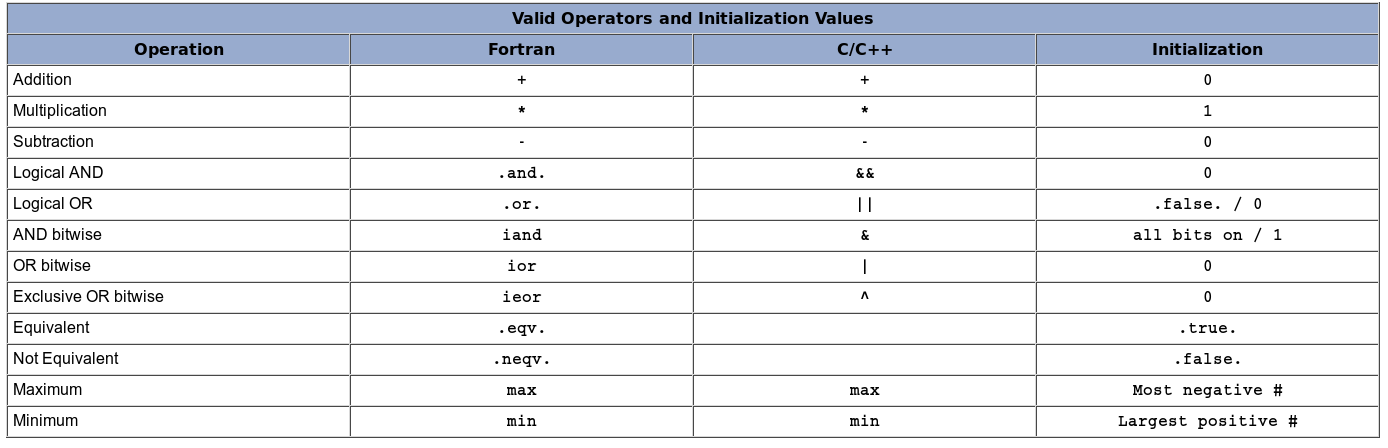
\includegraphics[height=7cm, width = \linewidth, keepaspectratio]{reduction.png}
\caption{opérateur de réduction}
\label{fig:reduction}
\end{figure}

\subsection{if}
La région visée n'est effectué en parallèle que si la condition est vraie. On se sert normalement de sa si la taille du problème est variable et qu'elle est trop petite.

\subsection{Nowait}
Lorsque les données sont indépendant, l'exécution de deux régions peut se chevaucher.\\
exemple:
\begin{lstlisting}[language=c]
#pragma omp parallel shared(n,a,b,c,d,e,f) private(i,scale)
{
	#pragma omp for nowait
	for (i=0; i<n; i++) a[i] = b[i] + c[i];
	#pragma omp for nowait
	for (i=0; i<n; i++) d[i] = e[i] + f[i];
	#pragma omp barrier
	scale = sum(a,0,n) + sum(d,0,n);
}
\end{lstlisting}

\subsection{Collapse}
On se sert du collapse pour indiquer le niveaux d'imbrication de nos boucles for. On peut augmenter le niveau de parallélisme avec sa.
\subsection{SIMD}
Directive pour les boucles indiquant qu'on veut déplacer le travail sur un processeur SIMD comme un GPU ou un vecteur. Toute fonction qui peut être appellé par du code SIMD doit petre déclarés SIMD (pragma omp declare SIMD). \\

Le compilateur devra assurer que le code visé pourra être compilé pour le processeur SIMD ciblé, par exemple avoir une copie en code natif et une copie en bytecode qui pourra être compilé à l'exécution pour le bon GPU.
\subsection{Safelen}
La distance maximale entre deux itérations qui seron exécutés en parallèle sur le dispositif SIMD.
\subsection{Aligned}
À combien d'octets sont alignés les variables listés
\subsection{Uniforme}
paramêtre d'une fonction SIMD qui ne varie pas d'un appel à l'autre de la même exécution SIMD concurrente.
\subsection{Target}
plusieurs utilisation:
\begin{itemize}
\item Target device: spécifier le dispositif SIMD à utiliser
\item Target data: spécifier les données à transférer vers/ du dispositif avec la clause map.
\item target update: synchroniser certaines données entre l'hôte et le dispositif SIMD.
\item Declare target: définir certaines variables sur le dispositif SIMD.
\end{itemize}

Exemple:
\begin{lstlisting}[language=c]
#define N 10000
#define M 1024
#pragma omp declare target
float Q[N][N];
#pragma omp declare simd uniform(i) linear(k) notinbranch
float P(const int i, const int k) { return Q[i][k] * Q[k][i]; }
#pragma omp end declare target
float accum(void) {
	float tmp = 0.0;
	int i, k;
	#pragma omp target
	#pragma omp parallel for reduction(+:tmp)
	for (i=0; i < N; i++) {
		float tmp1 = 0.0;
		#pragma omp simd reduction(+:tmp1)
		for (k=0; k < M; k++) {
			tmp1 += P(i,k);
		}
		tmp += tmp1;
	}
	return tmp;
}

//ou..

#define THRESHOLD1 1000000
#define THRESHOLD2 1000
extern void init(float*, float*, int);
extern void output(float*, int);
void vec_mult(float *p, float *v1, float *v2, int N) {
	int i;
	init(v1, v2, N);
	#pragma omp target if(N>THRESHOLD1) map(to: v1[0:N], v2[:N])\
	map(from: p[0:N])
	#pragma omp parallel for if(N>THRESHOLD2)
	for (i=0; i<N; i++) {
		p[i] = v1[i] * v2[i];
	}
	output(p, N);
}

// ou encore..

extern void init(float *, float *, int);
extern int maybe_init_again(float *, int);
extern void output(float *, int);
void vec_mult(float *p, float *v1, float *v2, int N) {
	int i;
	init(v1, v2, N);
	#pragma omp target data map(to: v1[:N], v2[:N]) map(from: p[0:N])
	{ 
		int changed;
		#pragma omp target
		#pragma omp parallel for
		for (i=0; i<N; i++) p[i] = v1[i] * v2[i];
		changed = maybe_init_again(v1, N);
		
		#pragma omp target update if (changed) to(v1[:N])
		changed = maybe_init_again(v2, N);

		#pragma omp target update if (changed) to(v2[:N])
		#pragma omp target
		#pragma omp parallel for
		for (i=0; i<N; i++) p[i] = p[i] + (v1[i] * v2[i]);
	}
	output(p, N);
}
\end{lstlisting}
C'est commande sont mieux expliquer dans les documentations d'OMP (v4.0+)
\section{Fonctions de supports de threads}
\begin{itemize}
\item omp\_set\_num\_threads: spécifier le nombre de fils
d'exécution.
\item omp\_get\_num\_threads: nombre de fils d'exécution.
\item omp\_get\_max\_threads: nombre maximal possible de fils
d'exécution.
\item omp\_get\_thread\_num: numéro du fil courant.
\item omp\_get\_num\_procs: nombre de processeurs disponibles.
\item omp\_in\_parallel: dans une région parallèle?
\item omp\_set\_dynamic, omp\_get\_dynamic: ajustement
dynamique du nombre de fils d'exécution.
\item omp\_set\_nested, omp\_get\_nested: permission d'avoir une
région parallèle imbriquée avec possiblement plus de fils
d'exécution créés.
\item OMP\_STACKSIZE: taille des piles pour les fils d'exécution. Variable ?
\item omp\_get\_wtime: temps écoulé en secondes.
\item omp\_get\_wtick: résolution de l'horloge utilisée pour
omp\_get\_wtime.
\item omp\_set\_schedule, omp\_get\_schedule: static, dynamic, guided, auto sont les
stratégies possibles pour diviser les itérations de boucles entre les fils
d'exécution, avec une granularité spécifiée.
\item omp\_get\_thread\_limit: nombre maximal de fils disponibles pour le programme.
\item omp\_set\_max\_active\_levels, omp\_get\_max\_active\_levels: profondeur
maximale d'imbrication de régions parallèles.
\item omp\_get\_level, omp\_get\_active\_level: profondeur courante de régions
parallèles (actives) imbriquées.
\item omp\_get\_ancestor\_thread\_num: numéro du thread parent.
\item omp\_get\_team\_size(level): nombre de thread dans la région parallèle ancêtre.
\end{itemize}

\paragraph{Précautions}
Il faut faire attention au placement des variables partagés pour éviter le faux partage en cache. Il faut aussi s'assurer que les fonction appelées dans les section parallèle sont prévue pour sa.. (threadsafe).\\

Il faut accéder les matrices par colonne (dernier indice qui varie le plus vite) et finalement choisire des morceaux assez gros pourminimiser le surcoût de contrôle mais assez petit pour permettre d'équilibrer le travail de chaque fil.

\section{Exercices.}
\subsection{5.1}
\paragraph{Question}
Un outil de détection de problème de synchronisation vous indique une course
dans la section réalisée par votre co-équipier qui affirme que tout est correct. Qui
croire?
\begin{lstlisting}
found = 0;

#pragma omp parallel for
for(i = 0 ; i < n ; i++){ 
	if(a[i] == key) found = 1; 
}
if(found) { ... }

\end{lstlisting}
\paragraph{Réponse}
Un seul changement peut arriver, toujours le même, found=1. Il y a effectivement
une course mais le résultat final ne dépend pas de la course.

\subsection{5.2}
\paragraph{Question}
Votre co-équipier se plaint que votre programme ne profite pas de la performance
disponible en raison de la barrière implicite entre les deux boucles. Il veut les
mettre nowait ou dans des sections. Est-ce correct? Avez-vous mieux à proposer?
\begin{lstlisting}
#pragma omp parallel
{ 
	#pragma omp for
	for(i = 0; i < n; i++){ 
		a[i] = f1(i); 
	}
	#pragma omp for
	for(i = 0; i < n; i++){ 
		b[i] = a[i] + f2(i); 
	}

}
\end{lstlisting}
\paragraph{Réponse}
Avec un ordonnancement statique, nowait serait possible. Mieux encore, on peut
fusionner les deux boucles.
\begin{lstlisting}
#pragma omp parallel
{ 
	#pragma omp for
	for(i = 0; i < n; i++){ 
		a[i] = f1(i);
		b[i] = a[i] + f2(i);
	}
}
\end{lstlisting}

\subsection{5.3}
\paragraph{Question}
Votre co-équipier a modifié votre programme en ajoutant des nowait et obtient un
gain de performance appréciable mais ses résultats seront-ils corrects et fiables?

\begin{lstlisting}
#pragma omp parallel
{ 
	#pragma omp for schedule(static) nowait
	for (i=0; i<n; i++) c[i] = (a[i] + b[i]) / 2.0f;
	#pragma omp for schedule(static) nowait
	for (i=0; i<n; i++) z[i] = sqrtf(c[i]);
	#pragma omp for schedule(static) nowait
	for (i=1; i<=n; i++) y[i] = z[i-1] + a[i];
}
\end{lstlisting}

\paragraph{Réponse}
Entre les deux premières boucles, l'ordonnancement statique règle clairement le
problème. C'est aussi le cas pour la troisième boucle car tout est décalé de 1
(indice de boucle et accès de z); le même fil opérera sur la même valeur de z. Le
dernier nowait est inutile puisque c'est la dernière boucle du parallel.

\subsection{4.4}
\paragraph{Question}
Votre programme comporte une boucle dont la longueur de chaque itération varie
grandement. Discutez de différents mécanismes qui pourraient être utilisés pour
assurer néanmoins une bonne parallélisation.
\paragraph{Réponse}
Avec un ordonnancement de boucle dynamique ou guidé, possiblement avec
une granularité assez fine, le nombre d'itérations par fil sera ajusté
automatiquement.


\chapter{Contrôle des Années précédents.}
\section{Année 2016}
\subsection{1}
\paragraph{a)}
Question de probabilités. On utilise la formule fourni et on utilise celle dans les notes (chapitre1) pour pouvoir faire le calcul. \\
$p(t)^{100}$ ou 100 est le nombre de cluster.
\paragraph{b)}
Callgrind regarde les différentes fonctions utilisé par le programme, et sa nous donne de l'informations sur les fonctions comme le temps de calculs, les appels système, etc. On s'en sert pour voir ou mettre notre effort pour parallélisé notre programme.
\paragraph{c)}
TBB est plus performant, la différence était quand même grande. il gère lui même la répartition du travail et parallélise à généralement à grain plus fin que pThread.
\paragraph{d)}
On se sert de la loi d'Amdahl, voir note.
2.95 pour 4 coeur avec 0.88 parallelisable. 7.47 pour 64 coeurs
\subsection{2}
\paragraph{a et b}
voir notes.
\paragraph{c)}
Faut le changer,\\
quand on change de thread, sa ne dérange pas\\
quand on change de processus, il faut que notre TLB puisse se servir d'un étiquette (soit un TLB avancés). sinon, il doit le flusher.

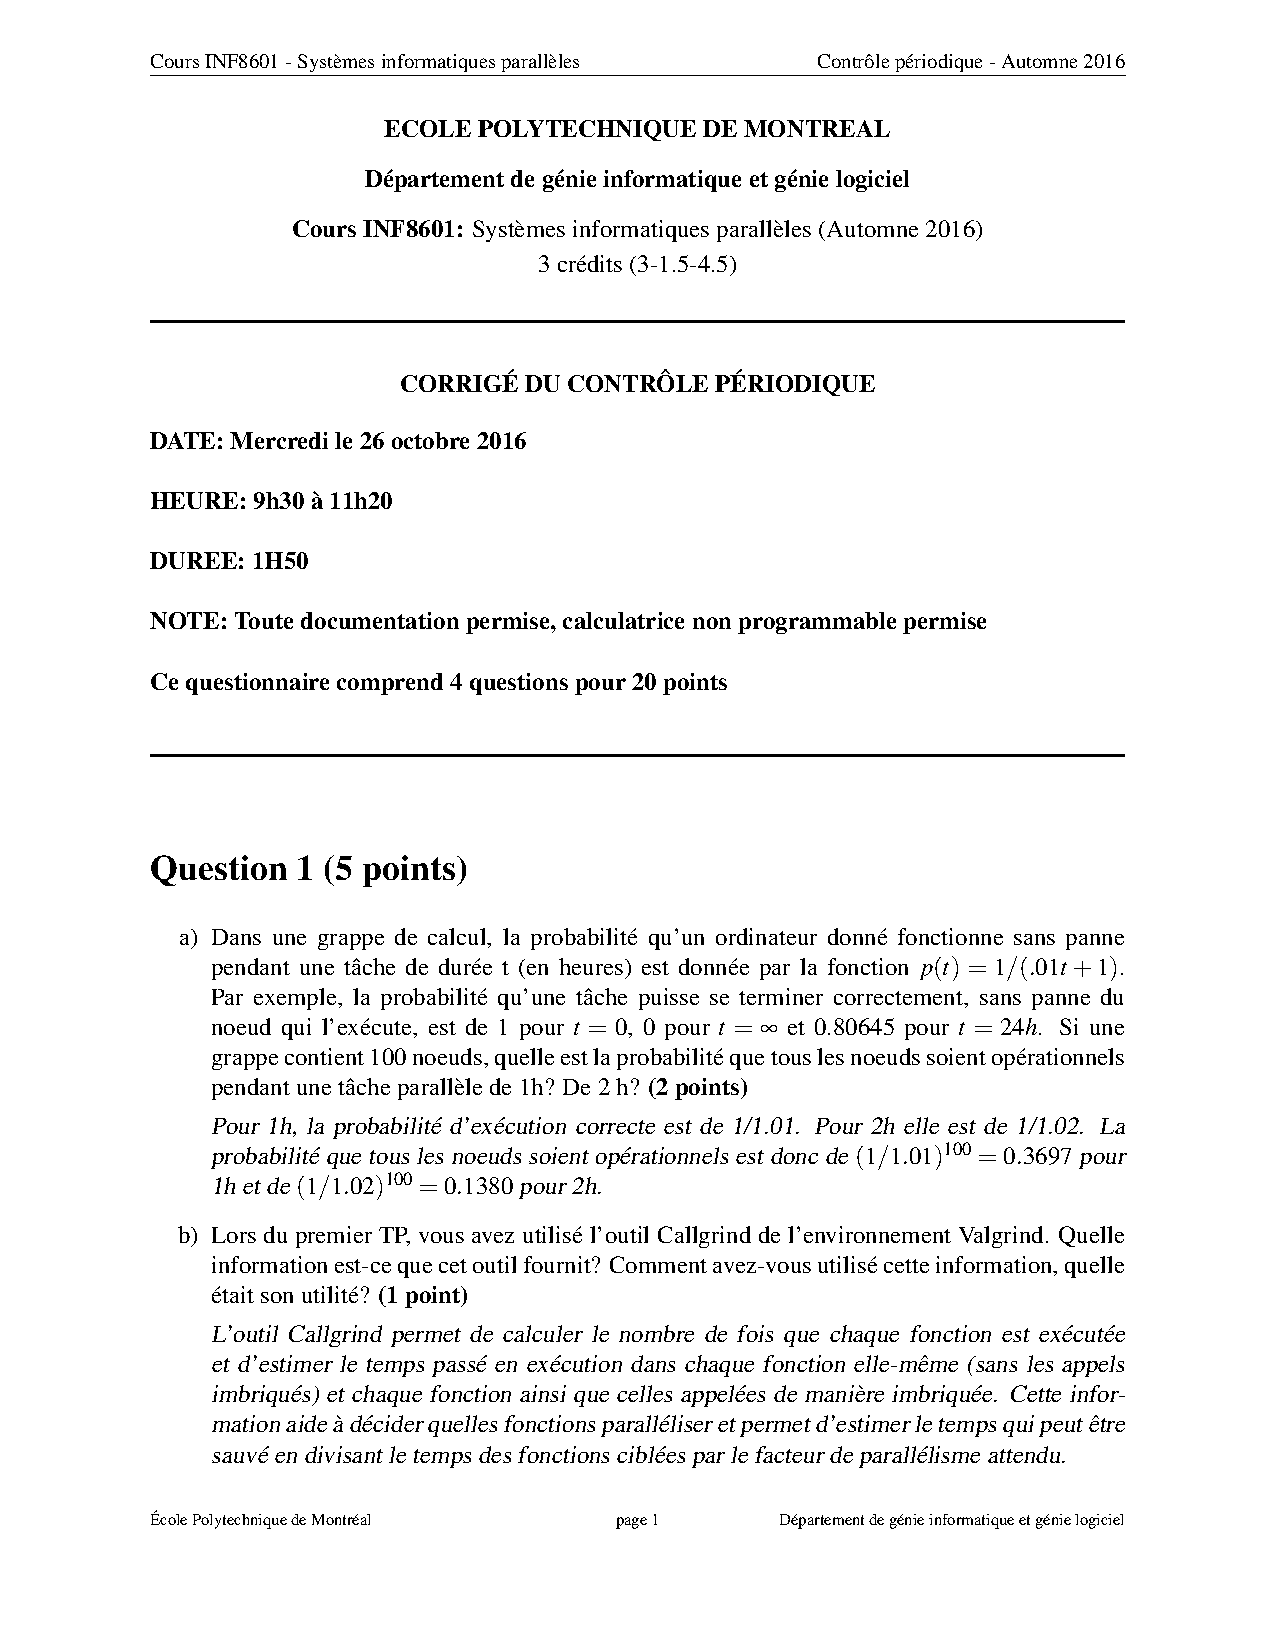
\includepdf[pages=-]{controleA2016C.pdf}
\section{Années 2014}
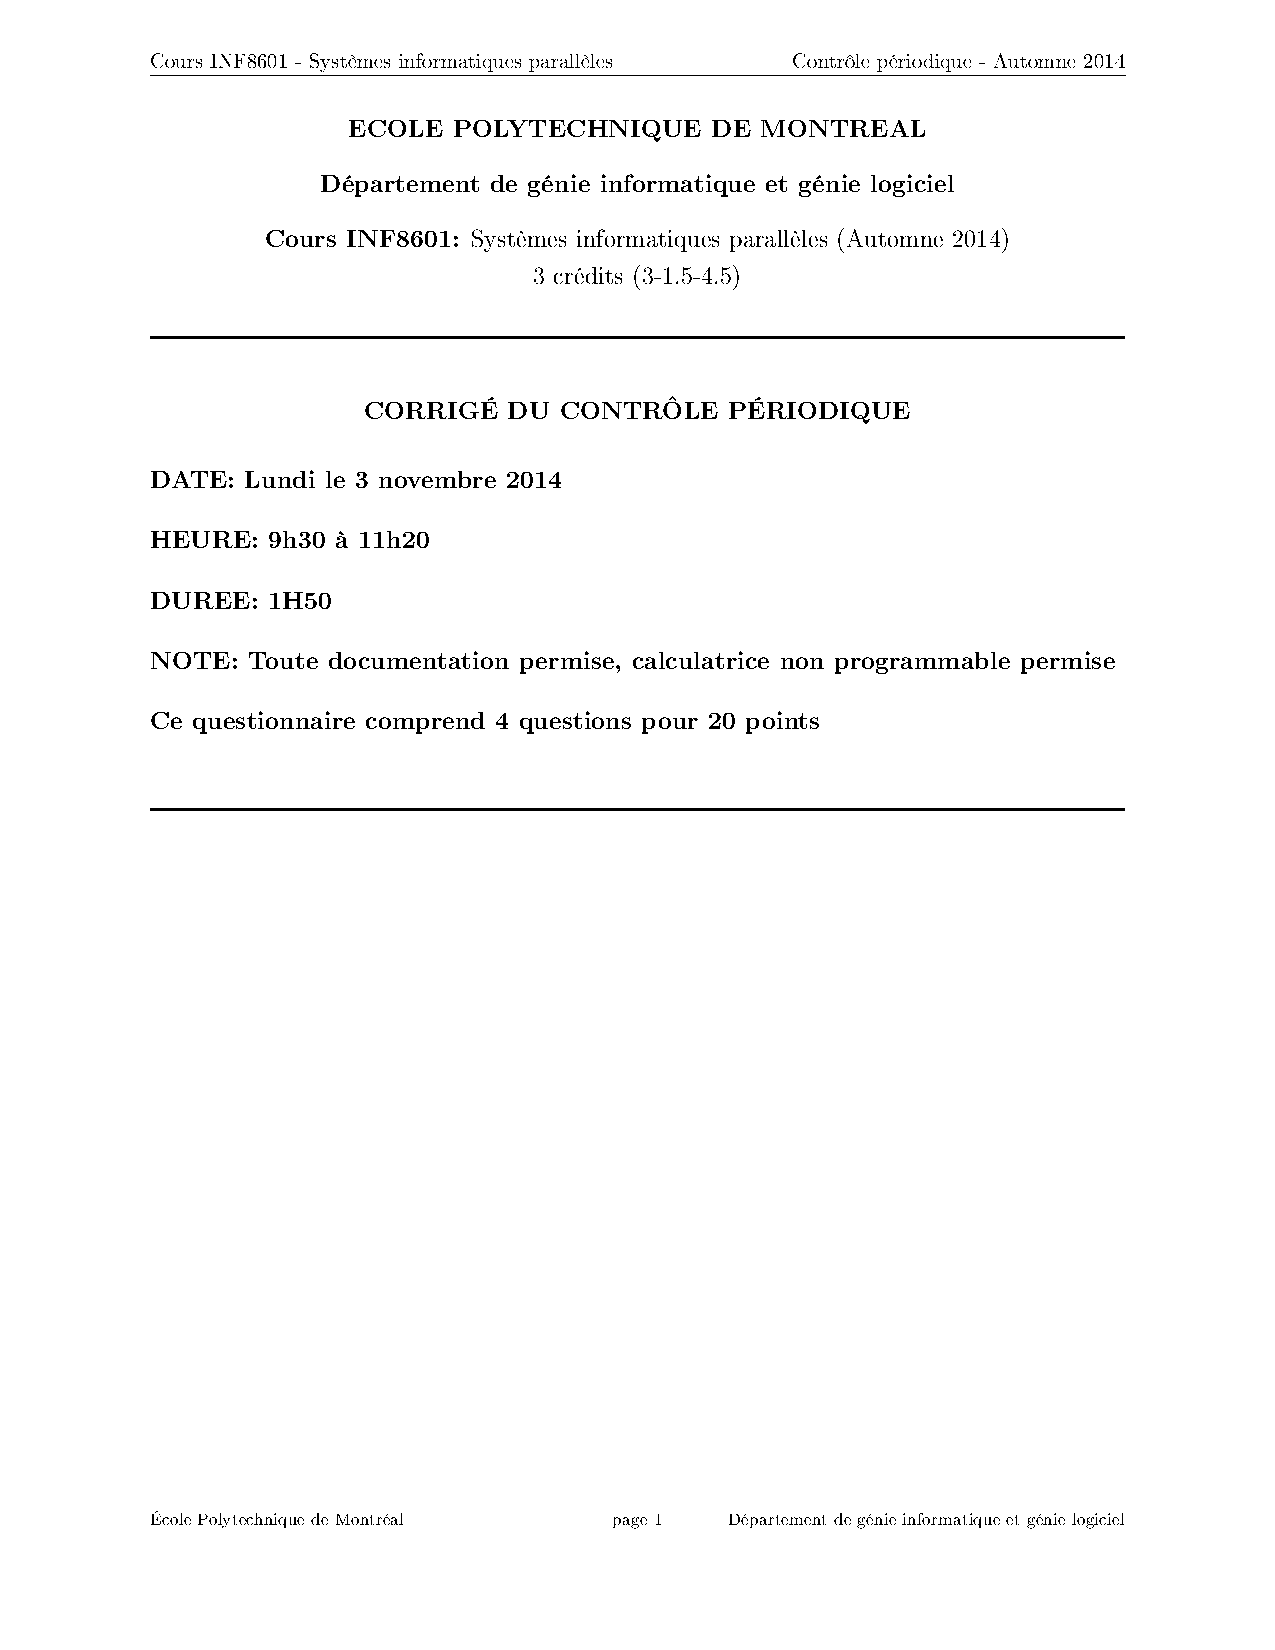
\includepdf[pages=-]{controleA2014C.pdf}
\section{Année 2013}
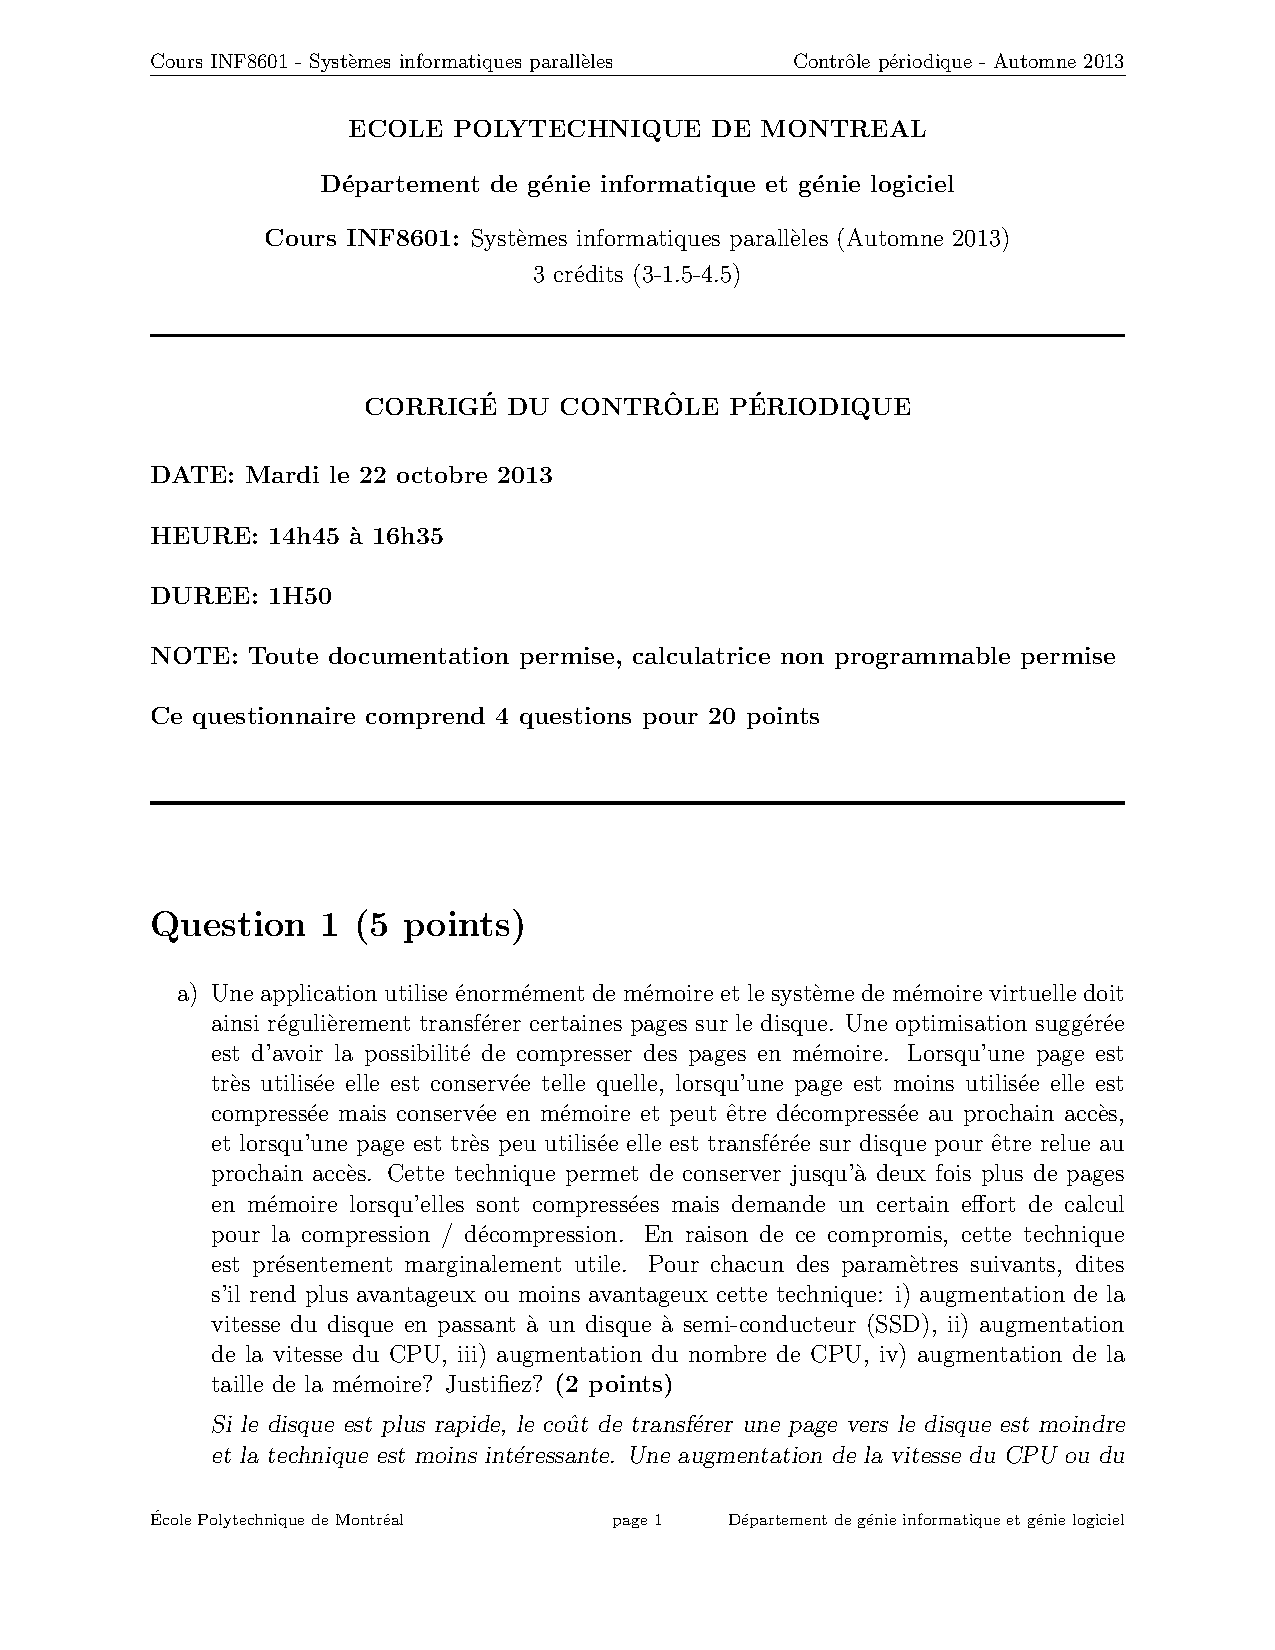
\includepdf[pages=-]{controleA2013C.pdf}
\section{Année 2012}
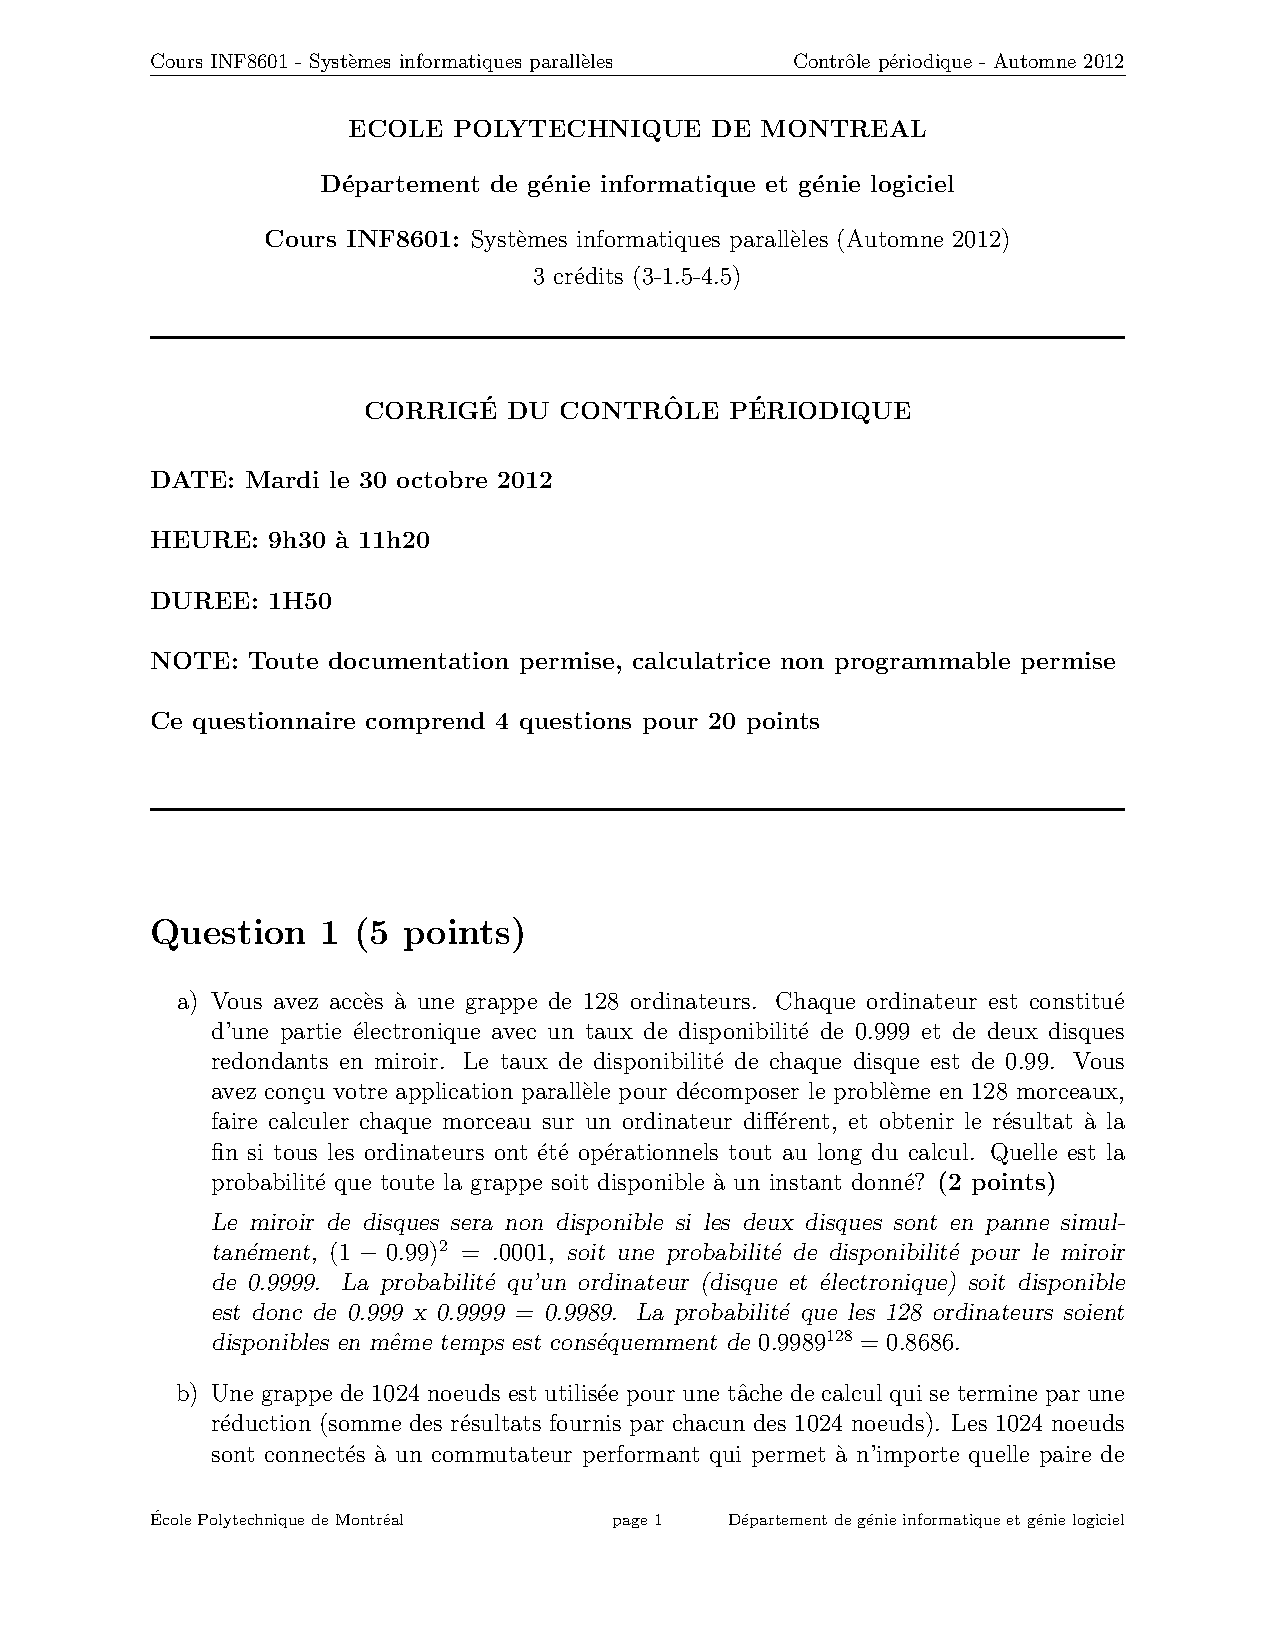
\includepdf[pages=-]{controleA2012C.pdf}

\chapter{MIPS - Assembleur Vectorielle}
Dans ce chapitre nous allons parler de processeur vectoriel. Ce sont des unités de processing qui ne sont pas nécessairement aussi populaire qu'avant, mais sa n'enlève pas de leur efficacité/puissance. Le principe c'est d'avoir plusieurs registre vectoriels (8 registres de 64 éléments de 64 bits scalaire) et de pacter plusieurs ALU (e.g. FP Add/Substract, FP Divide, Integer....) ayant chacune sa pipeline (un élément par cycle.\\

On fait un chargement et rangement à partir de la mémoire, en pipeline (un élément par cycle) avec un décalage de 1 ou plus entre les éléments ou par vecteur d'indirection.\\

On a aussi un registre de masque (64 bits) pour activer les opérations ou recevoir le résultat d'une comparaison.On a aussi un registre de longueur qui détermine le nombre d'éléments à traiter.\\

\begin{figure}[!ht]
\centering
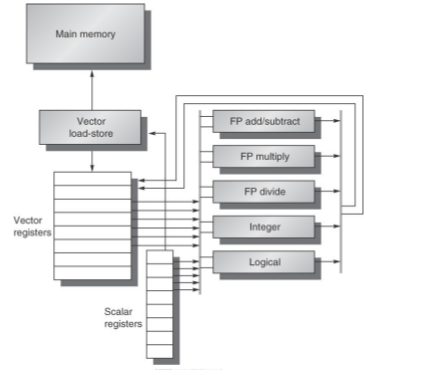
\includegraphics[width = 7cm]{processeur_vectoriel.png}
\caption{Configuration d'un processeur vectoriel}
\label{fig:layout_vectoriel}
\end{figure}

On caractérise les processeur vectoriel par:
\begin{itemize}
\item Une réduction du nombre d'instructions exécutées (instruction vectorielle
versus boucle).

\item Plusieurs instructions vectorielles peuvent s'exécuter presqu'en même
temps par chaînage si elles sont indépendantes ou si le résultat d'une est
directement pris par l'autre au cycle suivant avec le matérial adéquat.

\item Possibilité de 2 ou 4 voies pour chaque ALU, opérant sur 2 ou 4 éléments
en parallèle.

\item Attention à nb\_elements / nb\_voies versus profondeur du pipeline.
\item Goûlot d'étranglement vers la mémoire?
\end{itemize}

\begin{figure}[!ht]
\centering
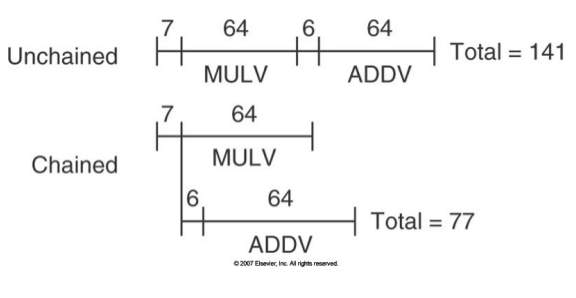
\includegraphics[width = 7cm]{exemple_pipeline.png}
\caption{Exemple de pipeline avec amélioration sur processeur vectoriel}
\label{fig:exemple_pipeline}
\end{figure}

Voici aussi le répartoire des instruction VMIPS:

\begin{figure}[!ht]
\centering
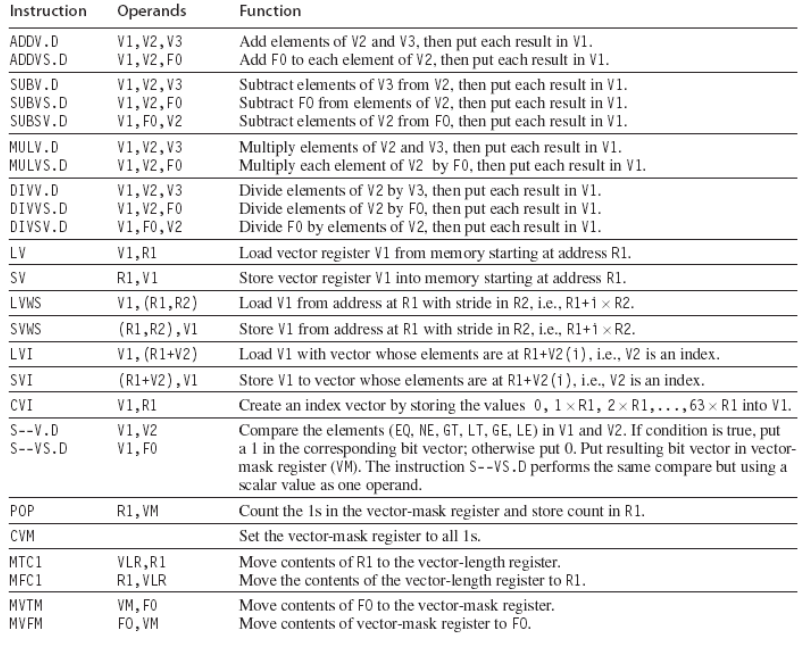
\includegraphics[width = \linewidth]{repertoire_mips.png}
\caption{Répertoire des instructions MIPS}
\label{fig:repertoire_mips}
\end{figure}

Le principe derrière vectoriser une boucle c'est de commencer par découper la boucle en morceaux de 64 éléments + un morceau de moins de 64 éléments. Ensuite on trouve les opérations vectoriels (les adds, les mult, les divide...). On fait ensuite la gestion des registres vectoriels et en remplacant les opérations conditioneles par des masques de contrôles des opérations vectorielles. En générale, sa fonctionne bien pour des boucles simples d'algèbres vectorielles.\\

Voici un exemple:
\begin{lstlisting}
for(i = 0; I < n; i++) Y[i] = a * X[i] + Y[i];
//on cherche a vectoriser cette boucles

low = 0;
vl = (n % 64)
// on fait une seule iterations qui fait moins de 64 et qui reste a se debarasser // du restant

//on itere le nombre initiales de la boucles diviser par 64, car on fait 64
//boucles a la fois. la premiere boucle s'effectue sur vl nombre d'iterations 
//car on veut faire le reste en premier. Apres la premiere boucle, on fixe 
//vl a 64 pour faire des pleines boucles

for(j = 0; j <= (n / 64); j++) {
	for(i = low; i < (low + vl); i++) {
		Y[i] = a * X[i] + Y[i];
	}
	//on incremente notre points de depart
	low = low + vl;
	/on place vl a 64 pour faire des pleines iterations
	vl = 64;
}

// maintenant, nous allons faire un exemple pour la gestion du control flow:

for(i = 0; i < 64; i++) {
	if(X[i] != 0) X[i] = X[i] - Y[i];
}


//on peut voir que on utilise un if pour verifier une certaines conditions, 
//pour le faire en assembleur:

//on charge nos valeurs dans nos registres V1 et V2 
//on store une valeur a 0 dans F0


LV		V1, Rx
LV		V2, Ry
L.D		F0, #0

// on compare V1 a F0, NE veut dire Not Equal, le S specifie qu'on le fait 
// sur un scalaire
SNEVS.D	V1, F0

// On soustrait V2 a V1 (V1-V2) et on le place dans V1 (V1 = V1-V2)
SUBVV.D	V1, V1, V2

// on store la valeur de V1 dans l'addresse memoire Rx
SV		V1, Rx

\end{lstlisting}

\section{Instructions multimédia}
On a eu un peu de vectorisation opportuniste avec certaines extensions Intel X86. on avait le MMX en 1996, c'étais des registre FP64 réutilisé pour 8 opérations de 8 bits ou 4 opérations de 16 bits.\\

On avait aussi le SSE en 99', 01', 04', 07' qui avait des registres de 128 bits pour 16 opérations de 8 bits, 6 de 16bits,4 de 32 bits, 2 de 64 bits.. 4 de 32 bits FP, 2 de 64 bits FP.. bref toute sorte de combinaison.\\

On avait finalement aussi l'AVX en 2010, ou c'étais des registres de 256 bits, avec le même principe. On fait de multiple opérations de 64, 32 bits dessus (plus de 8!!).\\

\section{Processeur Graphique}
Dans la même lignée, on a eu aussi l'ère des GPUs. Ce hardware est très puissants et peu dispendieux. C'est comme des super vecteurs à rabais. Le principe est de parallélisé des section de code (grid) décomposé en bloc de fils (thread blocs).\\

Chaque bloc est exécuté sur un processeur SIMD du GPU. Un processeur SIMD possède plusieurs (e.g. 32) ALU (thread processor) et gère plusieurs fils simultanément. Le processeur SIMD choisit la prochaine instruction du
prochain fil prêt et l'exécute sur ses 32 ALU.


\subsection{Mémoire}

Dans les GPU, on a:
\begin{itemize}
\item Mémoire privée: pour chaque ALU (résultats
intermédiaires).
\item Mémoire locale: mémoire locale à chaque processeur
SIMD.
\item Mémoire GPU: mémoire accessible à tous les processeurs
SIMD de même qu'au processeur hôte.

\item Un circuit filtre les accès mémoire pour regrouper les
accès à des adresses consécutives et les faire en pipeline
\end{itemize}

\subsection{Instructions}
Initialement, on avait les programmes en PTX (Nvidia), qui convertissait du code machine pour la carte spécifique au moment de l'exécution (pas très optimisé??).\\

Ces registres nous donnait accès à des opérations arithmétique: (s32, u32, f32, s64, u64, f64),
transcendentales (sqrt, sin...), logiques, accès mémoire,
opérations atomiques, contrôle (branch, call, ret, bar, exit).\\

Toutes les instructions peuvent être conditionnelles et
dépendre d'un bit d'activation dans un registre prédicat. Lorsque certains ALU font une branche IF, les autres sont
inactifs et sont réactivés pour le ELSE.\\

Une instruction vectorielle avec un élément par ALU, plutôt qu'une instruction vectorielle par ALU pendant 64 cycles en pipeline. Les nombreux fils (comme le Hyperthreading) compensent
pour la latence d'accès mémoire. Ceci fait en sorte que sa utilise un Modèle de programmation assez contraignant, plus difficile à
optimiser. C'est aussi beaucoup plus plus difficile à analyser la performance ou débogger étant donné que toute le stock se retrouve sur le GPU (pas de stdout/débug conventionel..).\\

Par contre, sa nous donne accès à du matériel puissant et peu dispendieux! Que nous allons discuter dans la section prochaine : \textbf{OPENCL}

\section{Éxercices}

Voici les éxercices pour la section MIPS:

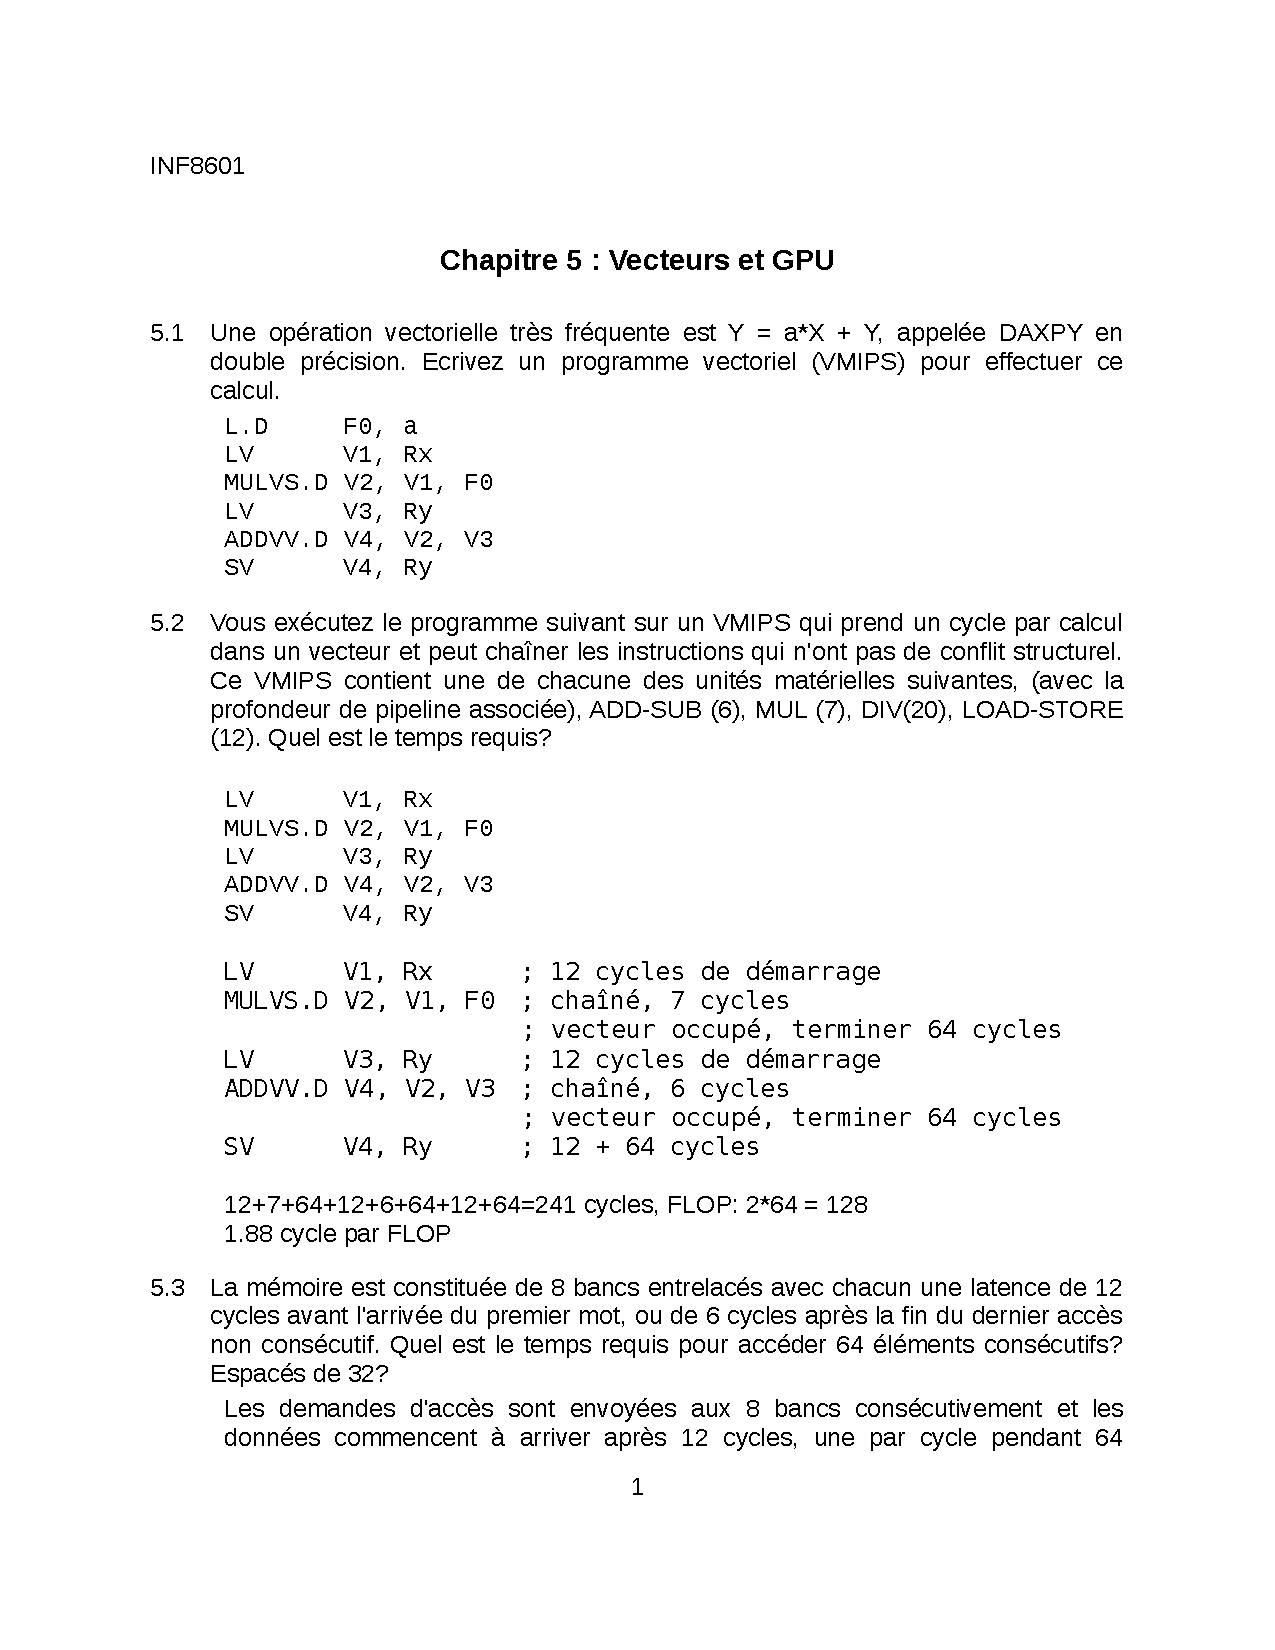
\includepdf[pages=-]{Solutions5-Vecteur.pdf}
\chapter{OpenCL}
Appelé le Open Computing Language, OpenCL à été proposé en 2008 par Apple après avoir été retravaillé avec l'aide de AMD, Intel, IBM et Nvidia. C'est un standard développé et maintenant par le consortium Khronos. La première version (1.0) à été released en 2008 avec la version 2.0 en 2013 qui a ajouter du C++. une intégration Vulkan, concept de priorités, minuteries.. \\

C'est supporté activement par AMD, IBM, Intel et aussi NVidia sous CUDA. \\

l'objectifs et de permettre d'utiliser les processeurs parallèles auxiliaires, unité vectorielles (MMX), processeurs graphique (GPGPU) et autres processeur de calcule et même les processeur dans les FPGA.. \\

Sa offre un environnement et langage normalisé pour utiliser de manière portable, ces systèmes parallèles hétérogène. C'est un standard ouvert avec implémentation de référence libre.\\

Le potentiel d'accélération d'OpenCL est très important.. (10 - 100 fois plus rapide !!). On le décrit comme des outils qui permettent aux programmeurs experts de faire des gains de vitesse appréciables pour les applications exigeantes. Le coute de développement est par contre important en temps et en complexité. \\

C'est aussi un outils de mise au point et d'analyse de performance spéfifique, et moins disponible et développés. 

Comme par exemple:
\begin{itemize}
\item Jeux
\item Logiciels de CAO,
\item Calculs Scientifique
\item craquer des codes de chiffrement (hacker)
\end{itemize}

\begin{figure}[!ht]
\centering
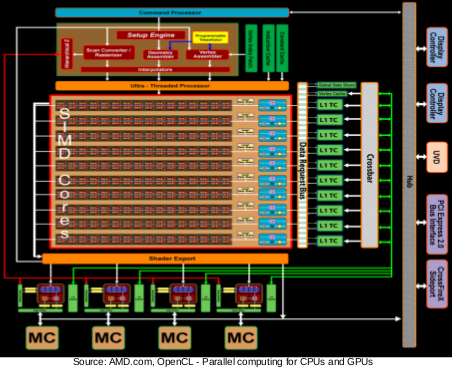
\includegraphics[width = 7cm]{ati_radeon.png}
\caption{Exemple du ATI Radeon HD4870}
\label{fig:ati_radeon_exemple}

\end{figure}
Voici une configuration typique d'un GPU AMD. le Radeon HD4870 comporte 10 processeur SIMD de 16 processeur de fil de 5 alu, total 800 ALU. Un milliard de transistor (1.2TFlops).\\

le 5870 lui, à 20 processeur SIMd de 16 processeur de fil de 5 ALU, deux fois plus d'ALU au total avec deux milliards de transistor et 2.7 TFlops de puissance.\\

Du côté de Nvidia, on à le GTX 480 avec 1.3 TFlops ainsi que le GTX 580 avec 1.6 TFlops..\\

Certains concepts important reste à retenir... 
\begin{itemize}
\item Ordinateur hôte (host), exécute le programme principal.
\item Dispositif de calcul (device), par exemple une carte graphique.
\item Un dispositif est constitué de processeurs SIMD (compute unit) qui
peuvent prendre en charge un ou des groupes de travail (work group).
\item Un processeur SIMD est constitué de plusieurs ALU (processing
element), chacun pouvant prendre un ou plusieurs item de travail
(work item).
\item Le programme principal définit des objets en mémoire (buffer, image),
des fonctions parallèles (kernel) et des événements (events). Il met en
queue les fonctions parallèles à exécuter.
\end{itemize}

Le modèle ressemble à ceci:
\begin{figure}[!ht]
\centering
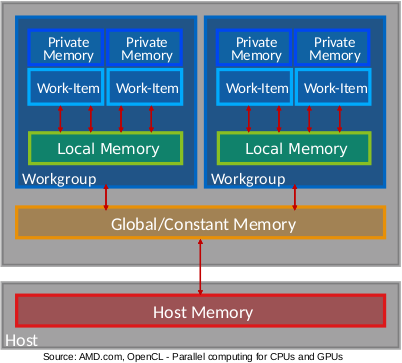
\includegraphics[width = 7cm]{opencl_memory.png}
\caption{Exemple de Modèle de Mémoire OpenCL}
\label{fig:OpenCL_Memory}
\end{figure}

\begin{figure}[!ht]
\centering
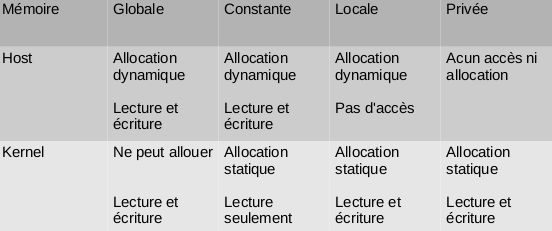
\includegraphics[width = 7cm]{opencl_table.png}
\caption{Modèle de Mémoire OpenCL}
\label{fig:OpenCL_Memory_Model}
\end{figure}

Il faut faire certaine distinction entre les différentes mémoire de la carte graphique. La mémoire global (DRAM) est très lente comparé à la mémoire local (SRAM). Une mémoire cache est inséré entre les deux. Le programme principal peut allouer des tampons (buffer)
ou images (2D et 3D).\\

Il peut aussi copier ou les calquer
entre sa mémoire et la mémoire globale du dispositif.\\

Par contre, Cohérence faible, des barrières mémoire sont requises
entre les opérations sur des mêmes éléments de données.\\

\subsection{Code}
Voici certaines exemples de code qui nous des opérations que nous pouvons faire avec les dispotifs/kernels:
\subsubsection{Commande abrégés}
Voici les fonctions primaires d'OpenCL abrégés selon mes notes prise en classe...

\begin{itemize}
\item oclGetPlatformID(): sa dit la platformes qu'on a acces

\item clGetDeviceIDs(): sadonne les ids de devices (du CPU et GPU)

\item clGetDeviceInfo() : sa donne l'info sur la devices

\item clCreateContext() : sa crée un contexte, genre une queue de commande est associer a un contexte et a un device

\item clCreateCommandQueu(): sa créer une queu de tache, associer a un device

\item plusieurs commandes comme retain/release et GetInfo qui sont universelle pour la majorité des contextes openCL\\

* faut faire beaucoup de gestion d'acces memoire en OpenCL *\\

CL\_DEVICE\_TYPE\_GPU spécifie qu'on cherche un GPU, n'importe lequel\\

\item createBuffer() : pas mal straight forward

\item createSubBuffer() : créer un sous-buffer d'un buffer

\item clenqueuReadBuffer() : command pour lire du tampon vers la mémoire hote, transfere GPU -­> CPU
\item clenqueuWriteBuffer() : contraire..

\item image = une forme de tampon, le but est d'inter-opérer avec OpenGL\\

les memes commands sont disponible pour les images..\\

le but :\\
\begin{itemize}
\item on créer les vecteurs (notre data)
\item on créer notre buffer pour nos variables en spécifiant read/write
\end{itemize}
	
	

\item clCreateProgrammeWithSource() : sa lit les fichiers OpenCL pour en faire un programme. on donne la source

\item clCreateProgrammewithBinary(): meme chose, mais on donne les binaire

\item une fois compilés:


\item clCreateKernel() : sa cherche ton programme, tu donne le pointeur vers ta fonction et ensuite sa fait ton kernel

\item clCreateKernelsInProgrmame() : sa cherche toute les fonctions d'un programme.

\item oclLoadProgSource() : sa load la source? un peu bizarre et pas dans l'API \\

le programme compile l'autre programme, alors il faut que tu check les erreurs

\item clBuildProgram() : sa batie ton programme avec le kernel et tout.

\item cl\_kernel : sa explique dans les notes

\item clEnqueuNDRangeKernel() :  ??

\item *cl\_event : evenements pour dire qu'on a fini*

\item cl\_enqueueNativeKernel(): soumettre une tache sur notrehote

\item cl\_CreateUserevent() : on créer un événement, qui peut etre utiliser pour faire dépendre d'autre trucs.

\item cl\_SetUsreEvent(): on change le statut

\item cl\_SetEventCallback(): associer une fonction a un callback

\item cl\_enQueueMarker() : pour mettre un marker dans la queu

\item cl\_enqueuBarrier(): ajouter une barriere, peu etre important pour mettre une forme de controle d'acces memoire

\item cl\_get\_profiling\_info(): sa donne l'information sur la queue.

\item cl\_flush(): saflush les commande

\item cl\_finish(): on termine..

\item workgroup = ? nombre de threads? sa depend de la carte graphique, il est possible de laisser le system determiner par lui-meme le workgroup size
\end{itemize}

\subsubsection{Accéder au dispositifs}
\begin{lstlisting}
/* notre ordinateur est la plate-forme */

cl_int oclGetPlatformID (cl_platform_id *platforms)

/* liste des dispositifs disponibles, usuellement 1 GPU
	on peut specifier le type chercher avec device type */
	
cl_int clGetDeviceIDs (cl_platform_id platform,
	cl_device_type device_type, cl_uint num_entries,
	cl_device_id *devices, cl_uint *num_devices)
	
/* Le device info donne l'information sur le nombre de
	workgroup ainsi que le nombre de work item sur le
	dispositif ainsi que le support 64 bits, les tailles
	d'images... */
	
cl_int clGetDeviceInfo (cl_device_id device, cl_device_info
	param_name, size_t param_value_size, void *param_value,
	size_t *param_value_size_ret)
\end{lstlisting}

\subsubsection{Contexte et Queue}
\begin{lstlisting}
/* Le contexte definit tout ce qui est associer a notre
	programmation sur ce dispositif pour un travail. */
	
cl_context clCreateContext (const cl_context_properties
	*properties, cl_uint num_devices, const cl_device_id
	*devices, void (*pfn_notify)(const char *errinfo...),
	void *user_data, cl_int *errcode_ret)
	
/* Une queue de commande permet d'envoyer le travail au GPU.
	La queue peut etre demander IN_ORDER ou non. On peut avoir
	plus d'une queue pour des taches independantes. */
	
cl_command_queue clCreateCommandQueue (cl_context context,
	cl_device_id device, cl_command_queue_properties
	properties, cl_int *errcode_ret)
\end{lstlisting}


\subsubsection{Exemple Complet: Device et Contexte}
\begin{lstlisting}
/* Initialiser le hardware, contexte et queue de commandes */
cl_int error = 0;
cl_platform_id platform;
cl_context context;
cl_command_queue queue;
cl_device_id device;

error = clGetPlatformID(&platform);
if (error != CL_SUCCESS) { ErrorExit(error); }

error = clGetDeviceIDs(platform, CL_DEVICE_TYPE_GPU, 1,
	&device, NULL);
if (err != CL_SUCCESS) { ErrorExit(error); }

context = clCreateContext(0, 1, &device, NULL, NULL, &error);
if (error != CL_SUCCESS) { ErrorExit(error); }

queue = clCreateCommandQueue(context, device, 0, &error);
if (error != CL_SUCCESS) { ErrorExit(error); }
\end{lstlisting}

\subsubsection{Gestion Mémoires}
Un tampon peut être créé pour lecture, écriture ou les deux.. (par les fonctions kernels).\\

Le tampon peut prendre la mémoire hôte spécifiée, allouer de la mémoire hôte ou allouer de la mémoire globale. La mémoire alloué peut être à partir d'une addresse hôte. \\

On peut définir un sous-tampon dans un tampon (inception ??)\\

Des commandes permettent de lire ou écrire, bloquant ou non, un tampon, sous-tampon ou section de tampon vers la mémoire hôte. ou vers un autre tampon.\\

Une commande permet de calquer un tampon sur la mémoire hôte.\\

Voici des exemples d'initialisation de Buffer

\begin{lstlisting}
/* creer un tampon */

cl_mem clCreateBuffer (cl_context context, cl_mem_flags flags,
	size_t size, void *host_ptr, cl_int *errcode_ret)

/* definir un sous-tampon */

cl_mem clCreateSubBuffer (cl_mem buffer, cl_mem_flags flags,
	cl_buffer_create_type buffer_create_type, const void
	*buffer_create_info, cl_int *errcode_ret)

/* commande pour lire du tampon vers la memoire hote */

cl_int clEnqueueReadBuffer (cl_command_queue command_queue,
	cl_mem buffer, cl_bool blocking_read, size_t offset,
	size_t cb, void *ptr, cl_uint num_events_in_wait_list,
	const cl_event *event_wait_list, cl_event *event)

/* commande pour ecrire de la memoire hote vers le tampon */

cl_int clEnqueueWriteBuffer (cl_command_queue command_queue,
	cl_mem buffer, cl_bool blocking_write, size_t offset,
	size_t cb,const void *ptr,cl_uint num_events_in_wait_list,
	const cl_event *event_wait_list, cl_event *event)
\end{lstlisting}

Une image dans le contexte d'OpenCL, peut être défini comme une sorte spécifique de tampons. On peut créer une image 2d ou 3d dans un des formats supportés (clGetSupportedImageFormats) avec une certaine tailles, its par couleur/pixels..\\

Des fonctions nous permettent d'accéder au contenu de l'image. Il est possible d'envoyer des commandes pour lire, écrire ou copier des images, avec la mémoire hôte, une autre image ou un tampon\\

Il est aussi possible de calquer une image en mémoire hôte... (calquer??)\\

\subsubsection{Programe hôte versus dispositif}
La plus grande partie du programme est en C ou C++ et est compilé pour l'hôte. Par contre, la parti qui s'exécute sur l'ALU, fonctions avec l'attribut kernel (ce qui va sur le dispositif), doit être compilée pour le bon dispositif à l'exécution. Elle peut être pré-compilé en langage intermédiaire pour réduire le surcout.\\

Le programme principale doit charger les fichiers OpenCL, les compiler et ensuite mettre en queu de commandes les fonctions kernel désirées.\\

Voici des exemples de commandes pour faire sa:\\

\begin{lstlisting}

/* Lire les fichiers OpenCL pour en faire un programme */

cl_program clCreateProgramWithSource (cl_context context,
	cl_uint count, const char **strings,const size_t *lengths,
	cl_int *errcode_ret)

/* Lire les fichiers OpenCL pre-compiler en IR
	pour en faire un programme */

cl_program clCreateProgramWithBinary (cl_context context,
	cl_uint num_devices, const cl_device_id *device_list,
	const size_t *lengths, const unsigned char **binaries,
	cl_int *binary_status, cl_int *errcode_ret)

/* Compiler le programme */

cl_int clBuildProgram (cl_program program,cl_uint num_devices,
	const cl_device_id *device_list, const char *options,
	void (CL_CALLBACK *pfn_notify)(cl_program program,
	void *user_data), void *user_data)
	
/* Obtenir le point d'entry d'une fonction specifier */

cl_kernel clCreateKernel (cl_program program, const char
	*kernel_name, cl_int *errcode_ret)

/* Obtenir toutes les fonctions */

cl_int clCreateKernelsInProgram (cl_program program,
	cl_uint num_kernels, cl_kernel *kernels,
	cl_uint *num_kernels_ret)

/* Specifier les arguments a associer a la fonction en vue
	de mettre en queue l'execution de cette fonction */

cl_int clSetKernelArg (cl_kernel kernel, cl_uint arg_index,
	size_t arg_size, const void *arg_value)
\end{lstlisting}

Et maintenant, voici un exemple complet qui match avec l'exemple précédent:
\begin{lstlisting}
size_t size;
const char* src = oclLoadProgSource("/tmp/abc.cl", "", &size);

cl_program pgm = clCreateProgramWithSource(context, 1, &src,
	&size, &error);
if(error != CL_SUCCESS) { ErrorExit(error); }

error = clBuildProgram(pgm, 1, &device, NULL, NULL, NULL);
if(error != CL_SUCCESS) { ErrorExit(error); }

char* bld_info;
clGetProgramBuildInfo(program, device, CL_PROGRAM_BUILD_LOG,
	0, NULL, &size);

bld_info = new char[size+1]; 
bld_info[size] = '\0';
clGetProgramBuildInfo(program, device, CL_PROGRAM_BUILD_LOG,
	size, bld_info, NULL);

cl_kernel abc_kernel=clCreateKernel(pgm,"abc",&error);
if(error != CL_SUCCESS) { ErrorExit(error); }
\end{lstlisting}

\subsubsection{Exécution de fonctions OpenCL}
On peut opérer sur des vecteurs pour tirer parti des nombreux ALU, différentes tâches peuvent aller sur les différents processeur et plusieurs tpaches peuvent être assigées au même processeur en hyper-threading.\\

 Exécuter une même fonction sur un grand nombre d'ALU dans plusieurs processeurs. Le travail peut être décrit sur 1, 2 ou 3 dimensions avec pour chaque dimensions un taille global et une taille locale. (eg. 1024X1024 versus 128X128)\\
 
Voici des exemples:
\begin{lstlisting}
/* Mettre en queue sur global size par groupe de local size */

cl_int clEnqueueNDRangeKernel (cl_command_queue command_queue,
	cl_kernel kernel, cl_uint work_dim, const size_t
	*global_work_offset, const size_t *global_work_size,
	const size_t *local_work_size, cl_uint
	num_events_in_wait_list, const cl_event *event_wait_list,
	cl_event *event)

/* Mettre en queue pour execution sur un processeur */

cl_int clEnqueueTask (cl_command_queue command_queue,
	cl_kernel kernel, cl_uint num_events_in_wait_list,
	const cl_event *event_wait_list, cl_event *event)

/* Mettre en queue sur un processeur de type hote */

cl_int clEnqueueNativeKernel (cl_command_queue command_queue,
	void (*user_func)(void *) void *args, size_t cb_args,
	cl_uint num_mem_objects, const cl_mem *mem_list,
	const void **args_mem_loc, cl_uint
	num_events_in_wait_list, const cl_event *event_wait_list,
	cl_event *event)
\end{lstlisting}

\subsubsection{Synchronisation par événements}
Le programme hôte peut créer des événements et changer leur status pour contrôler quand certaines commande pourront commencer. Il peut par exemple attendre après certains événement, ou il peut demander une fonction de rappel lors du changement d'état d'un événement. La fonction de rappel est très limitée dans ce qu'elle peut appeler.\\

Encore une fois, voici des exemples:
\begin{lstlisting}
/* Creer un evenement sur lequel faire dependre */

cl_event clCreateUserEvent (cl_context context, cl_int
	*errcode_ret)

/* Changer le statut a pret ou a erreur */

cl_int clSetUserEventStatus (cl_event event, cl_int
	execution_status)

/* Attendre apres des evenements */

cl_int clWaitForEvents (cl_uint num_events, const cl_event
	*event_list)

/* Associer une fonction de rappel a un evenement */

cl_int clSetEventCallback (cl_event event, cl_int
	command_exec_callback_type, void (CL_CALLBACK
	*pfn_event_notify)(cl_event event, cl_int
	event_command_exec_status, void *user_data),
	void *user_data)
\end{lstlisting}

\subsubsection{Barrières}
Les commandes dans une queus IN\_ORDER sont sérialisées et les résultats de la commande précédente sont disponible pour la suivante.\\

Les différentes commandes d'une queu OUT\_OF\_ORDER ou les commandes de queues distincte ne sont pas synchronisé. on peut mettre des marqueur pour savoir lorsque les commande précédentes d'une queue sont terminées.\\

On ajoute donc des barrières pour assurer que toutes les commande précédentes sont faite avant de commencer les suivantes. \\

Commande d'attente d'événements peut être mise en queue..\\

voici des exemples de barrières:\\

\begin{lstlisting}
/* Indique que toutes les commandes anterieures sont
	terminees */

cl_int clEnqueueMarker (cl_command_queue command_queue,
	cl_event *event)

/* Assure que toutes les commandes anterieures sont terminees
	avant que les commandes posterieures ne commencent */

cl_int clEnqueueBarrier (cl_command_queue command_queue)

/* Attend apres les evenements specifies avant de
	poursuivre */

cl_int clEnqueueWaitForEvents (cl_command_queue command_queue,
	cl_uint num_events, const cl_event *event_list)
\end{lstlisting}

\subsubsection{Divers}
On a aussi divers autre fonction OpenCL qui peuvent servir à plein d'autre chose..\\

l'événement de fin d'une commande peut contenir de l'info sur l'exécution: temps de mise en queu, soumission, début et fin.. Ceci permet de comprendre la performance de l'applicaiton. \\

 Lorsqu'une fonction de rappel met une commande en queu, celle-ci n'est pas soumise à ce moment. Il faut faire un flush sur la queue.\\
 
 On peut attendre pour la fin de l'exécution de toutes les commandes dans une queu (Finish).\\
 
 Voici des exemples:
 \begin{lstlisting}
 /* Extraire l'information sur le temps d'execution d'un
	evenement */

cl_int clGetEventProfilingInfo (cl_event event,
	cl_profiling_info param_name, size_t param_value_size,
	void *param_value, size_t *param_value_size_ret)

/* Activer la soumission des commandes de la queue */

cl_int clFlush (cl_command_queue command_queue)

/* Attendre que toutes les commandes en queue soient
	terminees */

cl_int clFinish (cl_command_queue command_queue)
 \end{lstlisting}
Voici des exemples complet d'exécutions (qui continue depuis la dernière exemple complet):
\begin{lstlisting}
error = clSetKernelArg(abc_kernel, 0, sizeof(cl_mem),
	&buffer_a);
error |= clSetKernelArg(abc_kernel, 1, sizeof(cl_mem),
	&buffer_b);
error |= clSetKernelArg(abc_kernel, 2, sizeof(cl_mem),
	&buffer_c);
error |= clSetKernelArg(abc_kernel, 3, sizeof(size_t), &size);

if(error != CL_SUCCESS) { ErrorExit(error); }

const size_t wg_size = 512;

const size_t total_size = ((1000000 / 512) + 1) * 512;

error = clEnqueueNDRangeKernel(queue, abc_kernel, 1, NULL,
	&total_size, &wg_size, 0, NULL, NULL);

if(error != CL_SUCCESS) { ErrorExit(error); }

clEnqueueReadBuffer(queue, buffer_c, CL_TRUE, 0, buffer_size,
	c, 0, NULL, NULL);
\end{lstlisting}

Suivit d'un exemple complet de finalisaton:
\begin{lstlisting}
delete[] a;
delete[] b;
delete[] c;
clReleaseKernel(abc_kernel);
clReleaseCommandQueue(queue);
clReleaseContext(context);
clReleaseMemObject(buffer_a);
clReleaseMemObject(buffer_b);
clReleaseMemObject(buffer_c);
\end{lstlisting}

\subsection{Fonctions Kernels - Sur Dispositif}
Les kernels OpenCL sont fait avec un sous-ensemble du C99 (très vieux). Avec des extensions spécifiques dans un fichier .cl\\

On utilise des types scalaires usuels, des bool, des char, short, int, long, signés ou non.. float, half, double, size\_t, ptr\_diff, intptr\_t.\\

Même types vectoriels  (de 2,3,4,6,8,16 éléments)\\

Par défaut, les composantes d'un vecteur de 4 sont x,y,z et w (quaternion??).\\

Exemples:
\begin{lstlisting}
float4 pos = (float4)(1.0f, 2.0f, 3.0f, 4.0f);
pos.xw = (float2)(5.0f, 6.0f);
pos.xyz = (float3)(3.0f, 5.0f, 9.0f);

a.xyzw = f.s0123;

float4 vf;
float2 low = vf.lo;
float2 high = vf.hi;
float2 even = vf.even;
float2 odd = vf.odd;

uchar4 u;
int4 c = convert_int4(u);

float f;
int i = convert_int(f);

union{ float f; uint u; double d;} u;
\end{lstlisting}
\subsubsection{Les opérateurs mathématique}
Les opérateurs mathématiques sont usuel, relations logiques et comparaisons sur les scalaires, scalaires-vecteurs et vecteurs-vecteurs. \\

La plupart des fonctions usuelles, incluant les fonction trigo sont ofertes et fonctionnent avec des vecteurs.\\

Fonctions pour lire ou écrire un vecteur à partir d'un pointeur.\\

Voici des exemples encore une fois:
\begin{lstlisting}
float4 u, v;
float f;

v = u + f;

u = atan2(v);

float distance(floatn p0, floatn p1)

float length(floatn p)

float8 vload8(size_t offset, const __local float *p)

void vstore8(float8 data, size_t offset, __local float *p)
\end{lstlisting}
\paragraph{Attributs}
Variables dans 4 espaces distinct: \_\_global, \_\_local (partagé dans le workgroup), \_\_constant (lecture seulement),\_\_private (par défaut, pour le workitem).\\

Les types image2d\_t et image3d\_t sont des objets \_\_global.\\

Arguments read\_only ou write\_only pour les fonctions kernels.\\

Peut spécifier l'alignement, \_\_attribute\_\_((aligned(8)))\\

\begin{lstlisting}
__global float4 *color;
typedef struct {
	float a[3];
	int
	b[2];
} foo_t;

__global foo_t *my_info;
__kernel void my_func(...)
{
	__local float a;
	__local float b[10];
	float c;
...
}
\end{lstlisting} 

\subsubsection{Synchronisation}
On peut utiliser des barriers pour assurer la synchronisation des différents points dans le processus. on utiliser les méthode suivantes pour insérer différentes barrière dans notre programme:\\

\begin{itemize}
\item void barrier (cl\_mem\_fence\_flags flags): synchroniser tous les workItem du workGroup.
\item void mem\_fence (cl\_mem\_fence\_flags flags)
\item void read\_mem\_fence (cl\_mem\_fence\_flags flags)
\item void write\_mem\_fence (cl\_mem\_fence\_flags flags)
\item Tous les exemple de fence sont des barrière mémoires pour les lectures ou écriture en mémoire du workitem.
\end{itemize}
On peut faire aussi une copie asynchrone entre la mémoire locale et globale. Un peut comme un événmenet est associé à chaque opération et peut être utilisé par wait\_group\_events.\\

Opérations atomique (add, sub, xchg, inc, dec, cmpxchg, min, max, and, or, xor) sur des entiers ou float en mémoire local ou global\\

Lecture ou écriture d'un pixel d'une image 2d ou 3d.\\

Différentes modes d'accès (sampler\_t) pour les images.\\

En voici quelques exemples:\\

\begin{lstlisting}
/* Simple addition vectorielle c = a + b */

__kernel void abc_kernel (__global const float* buffer_a,
__global const float* buffer_b, __global float* buffer_c,
const int nb)
{
	/* Nous sommes en une seule dimension, l'index global nous
		indique l'element sur lequel travailler */
		
	const int id = get_global_id(0);

	/* Nous avons quelques work_item de plus que la var taille
		il faut donc s'assurer de ne pas depasser. */
	
	if (id < nb) buffer_c[id] = buffer_a[id] + buffer_b[id];
}
\end{lstlisting}

\section{Optimisation}
l'optimisation OpenCL se fait en :
\begin{itemize}
\item Minimiser les interactions entre l'hôte et le GPU.
\item Regrouper les accès mémoire consécutifs en lignes complètes
alignées.
\item Avoir un grand nombre de fils possibles sur chaque processeur
SIMD afin d'avoir toujours quelque chose à faire lors des
attentes pour la mémoire et le décodage des instructions.
\item Utiliser le matériel au maximum en tenant compte de la
capacité (mémoire locale, registres) des processeurs SIMD
\item Utiliser les instructions vectorielles (au moins jusqu'à taille 4).
\end{itemize}

En voici un exemple d'optimisation d'accès mémoire:
\begin{lstlisting}
/* c[m][n], OpenCL organiser en m*n */

int x = get_global_id(0);
int y = get_global_id(1);

c[x][y] = a[x] * b[y];

/* OpenCL organiser en n*m */

int x = get_global_id(1);
int y = get_global_id(0);

c[x][y] = a[x] * b[y];

/* get_global_id(0) varie le plus vite, il faut donc le mettre
	pour y, de maniere a faire des acces a des cases memoire
	consecutives en meme temps qui pourront etre regroupes.
	Peut etre plusieurs fois plus rapide! */
\end{lstlisting}
\paragraph{Maximisation du nombre d'items}
Le but est de déterminer le nombre de registre et la quantité de mémoire local requise par un workitem (par test?).\\

Selon la quantité de registre et de mémoire disponible sur un SIMD, cela détermine la taille du WorkGroup.\\

De cette manière, on maximise le nombre de fils possible sur chaque processeur SIMD, en permettant de maintenire le matériel toujours occupé.\\

On suppose que la tallle total divisé par la taille de Work Group est largement supérieur au nombre de SIMD.

\paragraph{Vectorisation}

L'augmentation du nombre de Work Item est plus fiable
que l'utilisation d'opérations vectorielles pour augmenter la
performance.\\

Une instruction vectorielle fait des accès mémoire
regroupés et demande une seule instruction.\\

Sur processeur Intel ou sur GPU AMD, les vecteurs float4
sont traités efficacement car certains éléments travaillent
sur 4 mots à la fois.\\

\section{Exemple TP2}
À FAIRE...

\begin{lstlisting}
int create_buffer(int width, int height)
{
    /*
     * TODO: initialiser la memoire requise avec clCreateBuffer()
     */

    cl_int ret = 0;
    output = clCreateBuffer(context,CL_MEM_WRITE_ONLY,width*height*sizeof(unsigned char)*3,NULL,&ret);
    ERR_THROW(CL_SUCCESS, ret, "clCreateBuffer failed");
    sinoscope = clCreateBuffer(context,CL_MEM_READ_ONLY,sizeof(sinoscope_t),NULL,&ret);
    ERR_THROW(CL_SUCCESS, ret, "clCreateBuffer failed");

    //goto error;
done:
    return ret;
error:
    ret = -1;
    goto done;
}

int opencl_init(int width, int height)
{
    cl_int err;
    char *code = NULL;
    size_t length = 0;

    get_opencl_queue();
    if (queue == NULL)
        return -1;
    load_kernel_code(&code, &length);
    if (code == NULL)
        return -1;

    /*
     * Initialisation du programme
     */
    prog = clCreateProgramWithSource(context, 1, (const char **) &code, &length, &err);
    ERR_THROW(CL_SUCCESS, err, "clCreateProgramWithSource failed");
    err = clBuildProgram(prog, 0, NULL, "-cl-fast-relaxed-math", NULL, NULL);
    ERR_THROW(CL_SUCCESS, err, "clBuildProgram failed");
    kernel = clCreateKernel(prog, "sinoscope_kernel", &err);
    ERR_THROW(CL_SUCCESS, err, "clCreateKernel failed");
    err = create_buffer(width, height);
    ERR_THROW(CL_SUCCESS, err, "create_buffer failed");

    free(code);
    return 0;
error:
    return -1;
}

void opencl_shutdown()
{
    if (queue) 	clReleaseCommandQueue(queue);
    if (context)	clReleaseContext(context);

    /*
     * TODO: liberer les ressources allouees
     */

    if (output) clReleaseMemObject(output);
    if (sinoscope) clReleaseMemObject(sinoscope);
    if (kernel) clReleaseKernel(kernel);
    if (prog) clReleaseProgram(prog);
}

int sinoscope_image_opencl(sinoscope_t *ptr)
{
    

    cl_int ret = 0;
    cl_event ev;
    if (ptr == NULL)
        goto error;

    size_t work_dim[2];
    work_dim[0] = ptr->width;
    work_dim[1] = ptr->height;

    ret = clEnqueueWriteBuffer(queue,sinoscope,CL_TRUE,0,sizeof(sinoscope_t),ptr,0,NULL,NULL);
    ERR_THROW(CL_SUCCESS, ret, "clEnqueueWriteBuffer failed");
    ret = clSetKernelArg(kernel,0,sizeof(cl_mem), &output);
    ERR_THROW(CL_SUCCESS, ret, "clSetKernelArg output failed");
    ret = clSetKernelArg(kernel,1,sizeof(cl_mem),&sinoscope);
    ERR_THROW(CL_SUCCESS, ret, "clSetKernelArg sinoscope failed");
    ret = clEnqueueNDRangeKernel(queue,kernel,2,NULL,work_dim,NULL,0,NULL,NULL);
    ERR_THROW(CL_SUCCESS, ret, "clEnqueueNDRangeKernel failed");
    ret = clFinish(queue);
    ERR_THROW(CL_SUCCESS, ret, "clFinish failed");
    ret = clEnqueueReadBuffer(queue,output,CL_TRUE,0,ptr->buf_size,ptr->buf,0,NULL,NULL);
    ERR_THROW(CL_SUCCESS, ret, "clEnqueueReadBuffer failed");

done:
    return ret;
error:
    ret = -1;
    goto done;
}
\end{lstlisting}

\section{Exercices}
Voici la feuille d'exercice:

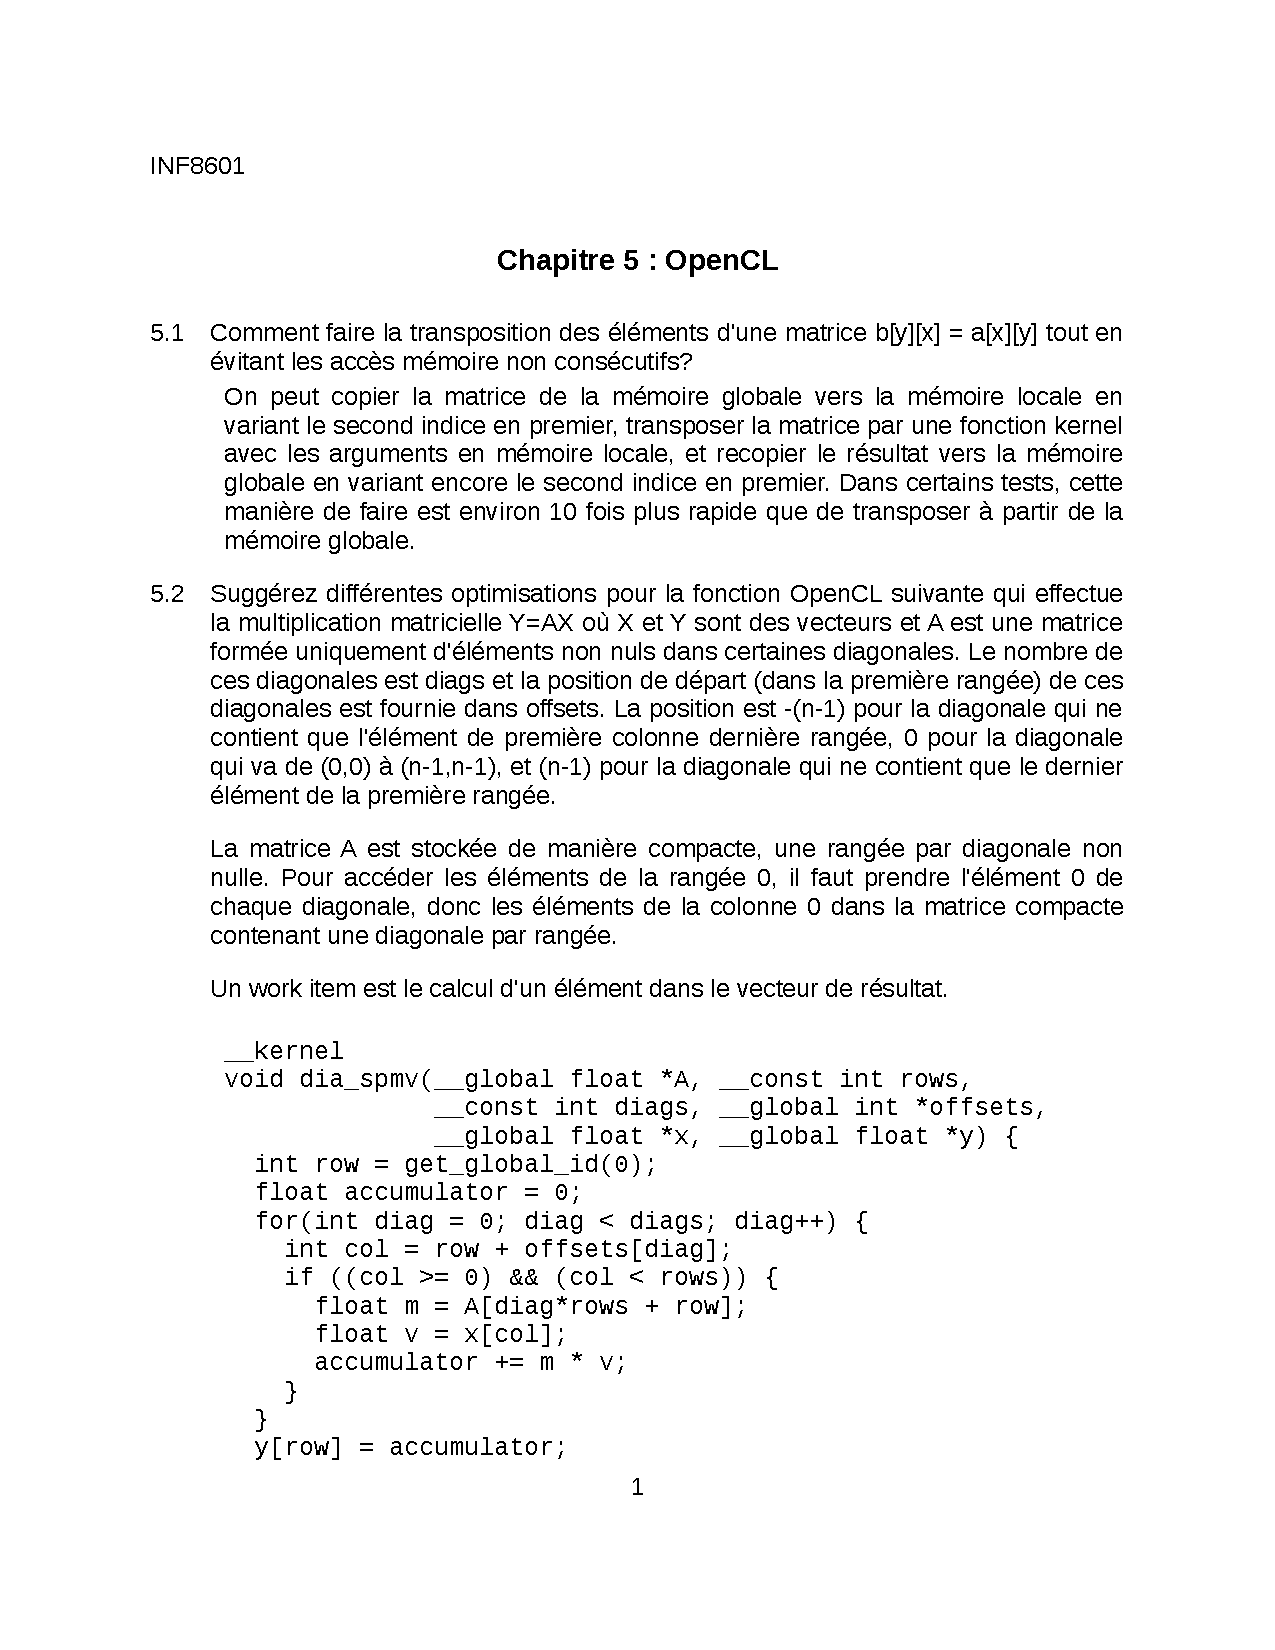
\includepdf[pages=-]{Solutions5-OpenCL.pdf}

\chapter{MPI}

discuté lors d'un workshop en 1992, MPI est l'approche classique du calcul parallèle distribués. La première version à été émise en 1993, la version finale en 1994. C'est un API de programmation parallèle sur multi-ordinateur (plusieurs noeuds avec plusieurs processeur). C'est une librairie qui sert à gérer les communication entre les différents noeuds afin qu'ils puissent s'envoyer des message et puissent travailler sur un problème de manière efficace. Sa bénéficie de l'expérience avec les systèmes antérieures (PVM, LINDA). \\

C'est un ensemble cohérent de fonctions permettant une interface simple tout en s'assurant que l'implémentation sous-jacente puisse être efficace. \\

Sa donne aussi une interopérabilité avec OpenMP et OpenCL. Par contre, la tolérance aux pannes est très faible..\\

Le public cible de la librairies sont toutes les grandes grappes de calcul, les laboratoires gouvernementaux (modélisation météo/nucléaire) ou industriel (analyse de réseaux de transmission chez l'hydro) et aussi modélisation par éléments finis chez bombardier ou Andritz.\\

Des version optimisées et outils sont offert par les grands fournisseurs de matériel. (Intel, IBM..)\\

Exemple d'un programme:
\begin{lstlisting}
#include "mpi.h"
#include <stdio.h>
int main( argc, argv )
int argc;
char **argv;
{
MPI_Init( &argc, &argv );
printf( "Hello world\n" );
MPI_Finalize();
return 0;
}
mpicc --mpilog --mpitrace -o hello hello.c
mpirun -np 2 hello
\end{lstlisting}

Le fonctionnement de base est :
\begin{enumerate}
\item d'initialiser la librairie
\item Utilisation du communicateur par défaut ou création du communicateur
\item Demander le nombre d'éléments N et sont ran (0 à N-1)
\item avec mpirun, le mee programme s'exécute sur N noeuds mais chaque instance fait un travail différent en se basant sur son rang qui la différencie.
\end{enumerate}

\section{Message et Types}
La librairie fonctionne en échangeant des messages selon le rang, comme par exemple des adresse, types d'éléments et nombre, plutôt que adresse et nombre d'octets..\\

Types sont définis récursivement pour représenter n'importe qu'elle structure de donnée. \\

Permet de spécifier les données telles qu'elle sont en minimisant la possibilité d'erreur sur la longueur.\\

Sa permet au système de faire les conversion si requis (e.g. petit ou gros boutien (endian))\\

voici les types d'MPI:
\begin{itemize}
\item Primitifs: MPI\_CHAR, MPI\_UNSIGNED\_CHAR (and SHORT, INT,
LONG), MPI\_FLOAT, MPI\_DOUBLE, MPI\_LONG\_DOUBLE...
\item Séquences: MPI\_TYPE\_CONTIGUOUS, MPI\_TYPE\_VECTOR,
MPI\_TYPE\_HVECTOR, MPI\_TYPE\_INDEXED,
MPI\_TYPE\_HINDEXED.
\item Agrégation: MPI\_TYPE\_CREATE\_STRUCT
\item Calcul de la position: MPI\_TYPE\_COMMIT
\item Divers: MPI\_TYPE\_FREE, MPI\_GET\_ADRESS,
MPI\_TYPE\_CREATE\_SUBARRAY,
MPI\_TYPE\_CREATE\_DARRAY, MPI\_PACK, MPI\_UNPACK
\end{itemize}
et en faisant la description de types:
\begin{lstlisting}
struct Element {
	unsigned temperature;
	double force[3];
	char status;
}
MPI_Datatype ElementType;
MPI_Datatype ElementFieldTypes[3] =
	{MPI_UNSIGNED, MPI_DOUBLE,MPI_CHAR};

int ElementFieldLength[3] = {1, 3, 1};

MPI_Aint ElementFieldPosition[3] =
	{0, sizeof(double), 4 * sizeof(double)};

MPI_Type_create_struct(3, ElementFieldLength,
	ElementFieldPosition, ElementFieldTypes, &ElementType);

MPI_Type_commit(&ElementType);
\end{lstlisting}

\subsubsection{Message}
En ce qui concerne les messages..\\

on les envoie avec les fonctions suivantes:\\

\begin{itemize}

\item Envoit bloquant:\\
\begin{itemize}
\item MPI\_SEND(buf, count, datatype, dest, tag, comm) bloque sur
l'envoi d'un message à dest.
\item MPI\_RECV(buf, count, datatype, source, tag, comm, status)
bloque sur l'attente d'un message de source avec tag ou
MPI\_ANY\_SOURCE, MPI\_ANY\_TAG.

\item MPI\_SENDRECV(sendbuf, sendcount, sendtype, dest, sendtag,
recvbuf, recvcount, recvtype, source, recvtag, comm, status)
aller-retour comme pour un appel de procédure.

\item MPI\_SENDRECV\_REPLACE(buf, count, datatype, dest, sendtag,
source, recvtag, comm, status) échange de données.
\end{itemize}

\item Envoit non bloquants:\\
\begin{itemize}
\item MPI\_ISEND(buf, count, datatype, dest, tag, comm, request)
l'envoi est demandé, buf ne doit plus être accédé jusqu'à ce
que l'envoi soit terminé.

\item MPI\_IRECV(buf, count, datatype, source, tag, comm, request)
la réception est demandée, buf ne peut être accédé avant que
la réception ne soit terminée.

\item MPI\_WAIT(request, status), MPI\_TEST(request, flag, status) ou
MPI\_REQUEST\_GET\_STATUS(request, flag, status) et
MPI\_REQUEST\_FREE(request) permettent de savoir lorsque
la requête est terminée.
\end{itemize}

\item Attente Multiple:\\
\begin{itemize}
\item MPI\_WAITANY(count, array\_of\_request, index, status),
MPI\_TESTANY(count, array\_of\_request, index, flag, status)
permet d'attendre après une de plusieurs requêtes.
\item MPI\_WAITALL(count, array\_of\_request, array\_of\_status),
MPI\_TESTALL(count, array\_of\_request, flag, array\_of\_status)
permet de vérifier toutes les requêtes.

\item MPI\_WAITSOME(incount, array\_of\_request, outcount,
array\_of\_index, array\_of\_status), MPI\_TESTSOME(count,
array\_of\_request, array\_of\_index, array\_of\_status) permet de
vérifier une ou plusieurs requêtes.
\end{itemize}

\item Autres fonctions sur les requêtes:\\
\begin{itemize}
\item MPI\_PROBE(source, tag, comm, status),
MPI\_IPROBE(source, tag, comm, flag, status), attend ou
vérifie si un message est disponible.
\item MPI\_CANCEL(request) annule une opération,
MPI\_TEST\_CANCELLED(status, flag) permet de le
vérifier.
\end{itemize}

\item Communications pré-définis:\\
\begin{itemize}
\item MPI\_SEND\_INIT(buf, count, datatype, dest, tag, comm,
request), MPI\_RECV\_INIT(buf, count, datatype, source,
tag, comm, request), spécifie les arguments pour un
envoi/réception à venir, et à répéter.

\item MPI\_START(request), MPI\_STARTALL(count,
array\_of\_request), démarre la requête.
\end{itemize}
\item Autres types d'envoie:\\

\begin{itemize}
\item MPI\_BSEND: buffered. Le contenu est copié avant d'être
envoyé.

\item MPI\_SSEND: synchronous. Ne peut se compléter avant
que le receveur ait commencé à recevoir le message.

\item MPI\_RSEND: ready, le receveur doit déjà être en attente
du message. Ceci peut permettre de faire l'envoi en étant
assuré qu'un tampon est prêt à l'autre bout.
\item MPI\_IBSEND, MPI\_ISSEND, MPI\_IRSEND,
MPI\_BSEND\_INIT, MPI\_SSEND\_INIT, MPI\_RSEND\_INIT.
\end{itemize}
\item Gestion manuelle des Tampons:\\

\begin{itemize}
\item MPI\_BUFFER\_ATTACH(buffer, size) spécifier
manuellement l'espace à utiliser pour les tampons et
conséquemment sa taille.
\item MPI\_BUFFER\_DETACH(buffer, size).
\end{itemize}
\end{itemize}

Voici un exemple de multiplication de matrice:\\
\begin{lstlisting}
#include "mpi.h"
#include <stdio.h>
#include <stdlib.h>
#define RA 62
#define CA 15
#define CB 7
#define ROOT 0
#define ROOT_A_FEUILE 1
#define FEUILLE_A_ROOT 2

int main (int argc, char *argv[]){
	int size, rank, src, dest, mtype;
	int rangees, moyenne, extra, offset, i, j, k, rc;
	double a[RA][CA], b[CA][CB], c[RA][CB];
	MPI_Status status;
	
	MPI_Init(&argc,&argv);
	MPI_Comm_rank(MPI_COMM_WORLD,&rank);
	MPI_Comm_size(MPI_COMM_WORLD,&size);
	
	if (rank == MASTER){ 
		moyenne = RA / (size - 1); extra = RA % (size - 1);
		offset = 0; mtype = ROOT_A_FEUILLE;
		for (dest=1; dest<=(size - 1); dest++){ 
			rangees = (dest <= extra) ? moyenne+1 : moyenne;
MPI_Send(&offset,1,MPI_INT,dest,mtype,MPI_COMM_WORLD);
MPI_Send(&rangees,1,MPI_INT,dest,mtype,MPI_COMM_WORLD);
MPI_Send(&a[offset][0],rangees*CA,MPI_DOUBLE,dest,
mtype, MPI_COMM_WORLD);

MPI_Send(&b,CA*CB,MPI_DOUBLE,dest,mtype,MPI_COMM_WORLD);
			offset = offset + rangees;
		}
		mtype = FEUILLE_A_ROOT;
		for (i=1; i<=(size - 1); i++){ 
			src = i;
MPI_Recv(&offset,1,MPI_INT,src,mtype,MPI_COMM_WORLD,&status);
MPI_Recv(&rangees,1,MPI_INT,src,mtype,MPI_COMM_WORLD,&status);
MPI_Recv(&c[offset][0],rangees*CB,MPI_DOUBLE,src,mtype,
MPI_COMM_WORLD,&status);
		}
	}
	
	if (rank > MASTER){ 
		mtype = ROOT_A_FEUILLE;
MPI_Recv(&offset,1,MPI_INT,ROOT,mtype,MPI_COMM_WORLD,&status);
MPI_Recv(&rangees,1,MPI_INT,ROOT,mtype,MPI_COMM_WORLD,&status);
MPI_Recv(&a,rangees*CA,MPI_DOUBLE,ROOT,mtype,MPI_COMM_WORLD,
&status);
MPI_Recv(&b,CA*CB,MPI_DOUBLE,ROOT,mtype,MPI_COMM_WORLD,&status);
		for (k=0; k<CB; k++)
			for (i=0; i<rangees; i++){ 
				c[i][k] = 0.0;
				for (j=0; j<CA; j++)
					c[i][k]=c[i][k]+a[i][j]*b[j][k];
			}
		mtype = FEUILLE_A_ROOT;
MPI_Send(&offset,1,MPI_INT,ROOT,mtype,MPI_COMM_WORLD);
MPI_Send(&rangees,1,MPI_INT,ROOT,mtype,MPI_COMM_WORLD);
MPI_Send(&c,rangees*CB,MPI_DOUBLE,MASTER,mtype,MPI_COMM_WORLD);
	}
	MPI_Finalize();
}
\end{lstlisting}

\subsection{Communications Globales}
Plusieurs moyens sont disponible pour faire de la communication globales sans avoir à gérer toutes les messages, en voici quelques une, de façon imager:\\

\begin{figure}[!ht]
\centering
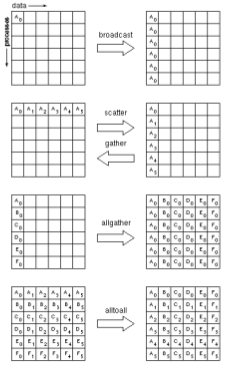
\includegraphics[width = 5cm]{global_comms.png}
\caption{communication globales}
\label{fig:global_comms}
\end{figure}

voici les différentes fonctions pour pouvoir effectuer les communications globals vu en haut.. les voici:\\
\begin{itemize}
\item Communications globales de base:\\
\begin{itemize}
\item MPI\_BARRIER(comm) bloque jusqu'à ce que tous les
membres du groupe aient appelé cette fonction.
\item MPI\_BCAST(buffer, count, datatype, root, comm) est
appelé par tous et le contenu de buffer sur le processus
de rang root est copié à tous les autres.
\item MPI\_GATHER(sendbuf, sendcount, sendtype, recvbuf,
recvcount, recvtype, root, comm) est équivalent à un send
de chaque processus (incluant root) et à n receive de root
avec l'adresse de réception calculée recvbuf + i * count.

\item MPI\_SCATTER(sendbuf, sendcount, sendtype, recvbuf,
recvcount, recvtype, root, comm) est équivalent à root qui
fait n send de sendbuf + i * sendcount et chaque
processus qui fait un receive.

\item MPI\_GATHERV, MPI\_SCATTERV, viennent avec un
vecteur de recvcount ou sendcount et un vecteur de
positions afin de recevoir ou d'envoyer des messages de
taille différente à une position variable.
\end{itemize}

\item méthodes tous à tous:\\
\begin{itemize}
\item MPI\_ALLGATHER(sendbuf, sendcount, sendtype, recvbuf,
recvcount, recvtype, comm) est comme un gather excepté que
tous les processus, il n'y a pas de root, recoivent toutes les
informations. MPI\_ALLGATHERV existe aussi

\item MPI\_ALLTOALL(sendbuf, sendcount, sendtype, recvbuf,
recvcount, recvtype, comm) chaque processus reçoit une
partie de ce qui est envoyé par chaque autre. Le bloc j envoyé
par le processus i est placé dans le bloc i du processus j.
MPI\_ALLTOALLV et MPI\_ALLTOALLW existent aussi.
\end{itemize}

\item Réduction:
\begin{itemize}
\item MPI\_REDUCE(sendbuf, recvbuf, count, datatype, op, root,
comm) les éléments de chaque processus sont combinés
ensemble dans l'élément correspondant du root avec
l'opération qui peut être MAX, MIN, SUM, PROD, LAND,
BAND, LOR, BOR, LXOR, BXOR, MAXLOC, MINLOC;
MAXLOC and MINLOC notent le processus qui fournit
l'élément maximal ou minimal. Il existe aussi
MPI\_ALLREDUCE qui retourne le résultat à tous.

\item MPI\_REDUCE\_SCATTER(sendbuf, recvbuf, recvcounts,
datatype, op, comm) distribue les réductions selon le
vecteur d'entier recvcounts.
\end{itemize}

\item Autres Fonctions:\\
\begin{itemize}
\item MPI\_SCAN(sendbuf, recvbuf, count, datatype, op, comm)
\item MPI\_EXSCAN, effectuent une réduction avec préfixe
inclusive (0 à i) ou exclusive (0 à i - 1).
\item MPI\_OP\_CREATE(function, commute, op) permet de
définir une opération en y associant une fonction.
\item MPI\_OP\_FREE relâche l'opération créée.
\end{itemize}
\end{itemize}

\section{Groupes de Communications}
On spécifie dans MPI dans différents groupe de communications. On peut spécifier nous mêmes notre topologies si c'est important. on utilise les fonctions suivantes pour définir nos groupes topologiques:\\

\begin{itemize}
\item Groupes de Communications:\\
\begin{itemize}
\item MPI\_GROUP\_SIZE(group, size), retourne la taille du groupe.
\item MPI\_GROUP\_RANK(group, rank), retourne la position dans le groupe.
\item MPI\_GROUP\_TRANSLATE\_RANKS(group1, n, ranks1, group2,
ranks2), pour chacun des n éléments du groupe 1 spécifiés
dans ranks1, retourne le rang correspondant de group2 dans
ranks2, ou MPI\_UNDEFINED s'il ne s'y trouve pas.
\item MPI\_GROUP\_COMPARE(group1, group2, result), compare les
groupes pour voir si c'est le même ou s'ils ont les mêmes
membres (IDENT, SIMILAR, UNEQUAL).
\end{itemize}
\item Sous-groupes:\\
\begin{itemize}
\item MPI\_COMM\_GROUP(comm, group) retourne le groupe du
communicateur.
\item MPI\_GROUP\_UNION(group1, group2, newgroup),MPI\_GROUP\_INTERSECTION,MPI\_GROUP\_DIFFERENCE combinent deux groupes
pour en faire un nouveau.
\item MPI\_GROUP\_INCL(group, n, ranks, newgroup),
MPI\_GROUP\_EXCL, sélectionner des éléments à inclure
ou exclure. RANGE\_INCL et RANGE\_EXCL existent aussi.
\end{itemize}

\item Autres Fonctions:\\

\begin{itemize}
\item MPI\_GROUP\_FREE(group), libère le groupe
\item MPI\_COMM\_COMPARE(comm1, comm2, result), vérifie si les
communicateurs (listes de membres) sont identiques, similaires
ou différents.
\item MPI\_COMM\_DUP(comm, newcomm), copie le communicateur.
\item MPI\_COMM\_CREATE(comm, group, newcomm), crée un
communicateur à partir d'un groupe.
\item MPI\_COMM\_SPLIT(comm, color, key, newcomm), crée un
communicateur pour chaque groupe de processus avec la même
couleur.
\end{itemize}

\item Attributs de communicateurs:\\
\begin{itemize}
\item MPI\_COMM\_CREATE\_KEYVAL(copy\_fn, delete\_fn, key,
fn\_data) réserve un code, key, pour un nouveau type
d'attribut. les fonctions fn\_copy et fn\_delete sont appelées
avec fn\_data lorsque l'attribut est copié ou relâché.

\item MPI\_COMM\_FREE\_KEYVAL(key)
\item MPI\_COMM\_SET\_ATTR(comm, key, value),
MPI\_COMM\_GET\_ATTR(comm, key, val, flag),
MPI\_COMM\_DELETE\_ATTR(comm, key), ajoute, accède
ou enlève un attribut sur un communicateur.
\end{itemize}
\item Intercommunications:\\
Communicateur entre deux groupes disjoints, local (inclut le
processus courant) et remote (l'autre groupe).
\begin{itemize}
\item MPI\_COMM\_TEST\_INTER(comm, flag),
MPI\_COMM\_SIZE/GROUP/RANK,
MPI\_COMM\_REMOTE\_SIZE/GROUP

\item MPI\_INTERCOMM\_CREATE(local\_comm, local\_leader,
bridge\_comm, remote\_leader, tag, newintercomm) doit être
appelé collectivement, bridge\_comm est un groupe englobant
dans lequel remote\_leader est identifié.
\item MPI\_INTERCOMM\_MERGE(intercomm, high, newintracomm)
\end{itemize}

\item Topologies Cartésiennes:\\
\begin{itemize}
\item MPI\_CART\_CREATE(comm\_old, ndims, dims, periods,
reorder, comm\_cart) crée un nouveau communicateur sur
lequel il sera facile de connaître les voisins selon une grille
à ndims dimensions (périodique, communication entre
premier et dernier, ou non).

\item MPI\_DIMS\_CREATE peut aider à choisir la grille.
\item MPI\_CARTDIM\_GET, MPI\_CART\_GET, permettent
d'interroger la structure de la grille.
\item MPI\_CART\_RANK(coom, coords, rank), retourne le rank d'une
coordonnée.
\item MPI\_CART\_COORDS(comm, rank, maxdims, coords), retourne les
coordonnées d'un rank.
\item MPI\_CART\_SHIFT(comm, direction, disp, rank\_source, rank\_dest),
calcule les voisins source et destination pour une communication
d'un déplacement et direction (dimension) spécifiés.
\item MPI\_CART\_SUB(comm, remain\_dims, newcomm) crée un
communicateur sur une topologie sur un sous-ensemble des
dimensions.
\end{itemize}

\item Topologies de Graphes:\\
\begin{itemize}
\item MPI\_GRAPH\_CREATE(comm\_old, nnodes, index, edges, reorder,
comm\_graph), crée un nouveau communicateur pour lequel il est
facile de savoir les voisins dans le graphe spécifié. Index dit où le
trouve la dernière arête dans edges connectée au noeud
correspondant.

\item MPI\_GRAPHDIMS\_GET, MPI\_GRAPH\_GET,
MPI\_GRAPH\_NEIGHBORS\_COUNT, MPI\_GRAPH\_NEIGHBORS,
permettent d'interroger la structure du graphe.

\item MPI\_TOPO\_TEST(comm, status), savoir si cartésien, graphe ou
aucun.
\end{itemize}

\item Récupération d'erreur:\\
\begin{itemize}
\item MPI\_COMM\_CREATE\_ERRHANDLER(fn, errhandler),
create a error handler from a pointer to function to call.

\item MPI\_COMM\_SET\_ERRHANDLER(comm, errhandler),
associer une fonction de rappel en cas d'erreur lors d'un
appel impliquant une communication.

\item MPI\_COMM\_GET\_ERRHANDLER

\item MPI\_ERRHANDLER\_FREE
\end{itemize}

\item D'autres fonctions utiles ..... :\\
\begin{itemize}
\item MPI\_PROCESSOR\_NAME(name, resultlen), nom du
noeud.
\item MPI\_WTIME() retourne le temps en secondes, double
précision.

\item MPI\_WTICK() retourne la résolution du temps en
secondes, double précision (e.g. .001s).
\end{itemize}
\end{itemize}

\section{Analyse de performance et optimisation}
Chaque version de fonction de MPI à une autre version qui peut faire de l'analyse de performance. Comme par exemple, la fonction MPI\_Send -> PMPI\_SEND. Cette nouvelle version fait de la stats et peut nous donner de l'info sur la performance.\\

\subsection{Optimisation}
Le principe pour optimiser les programmes MPI sont les suivants:\\
\begin{itemize}
\item Utiliser tous les noeuds, tout le temps (choisir la
granularité, équilibrer la charge).

\item Réduire la communication (grouper les messages,
recalculer, garder des copies).

\item Eviter les copies de données (e.g. BSend, données non
contiguës).

\item RECV avant SEND, communications asynchrones en
parallèle avec le calcul.

\item Requêtes réutilisées, éviter la scrutation..
\end{itemize}

Normalement, pour faire du profilage on trace tous les envois de message et blocages associés. VampirTRace est gratuit mais le visualisateur, Vampir, est commercial. \\

MPE/Jumpshot (Argonne National Lab), TAU (UofOregon, Los Alamos) ainsi que Paraver (Barcelona Supercomputing) sont des outils de trace. \\

Finalement, nous avons l'oracle Studio Performance Analyzer.\\

\section{Conclusion}

Pour conclure, MPI est relativement simple (en terme de commandes) et mature. Les grappes de noeuds n'ont pas changé aussi vite que les multi-processeurs. Il n'existe plus beaucoup d'équivalent en terme de compétition.. \\

La mise à l'échelle est cruciale avec les problèmes de tailles monstrueuses avec des grappes de milliers de noeuds. Par contre, pour certaines applications, Hadoop et Spark peuvent être considérer comme des alternatives.
\section{Éxercices}
Voici les Éxercices pour la section MPI

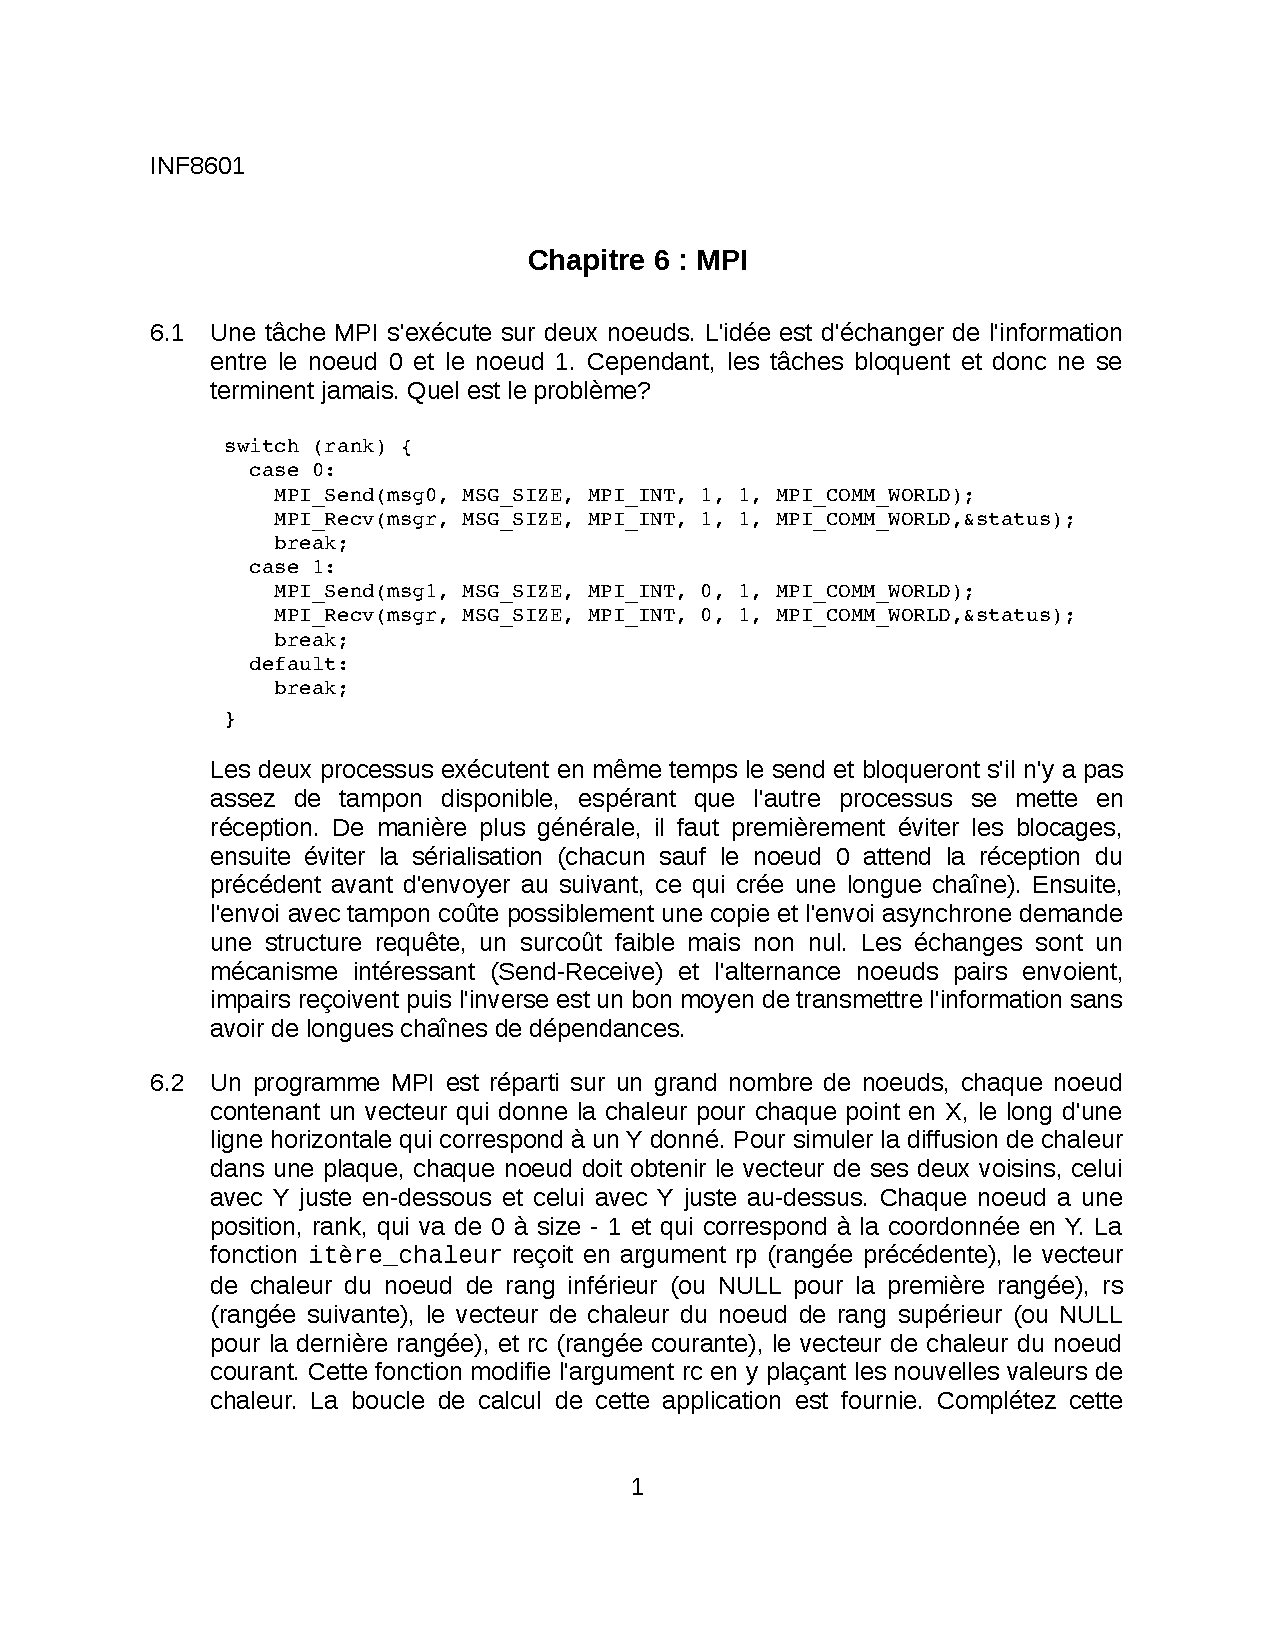
\includepdf[pages=-]{Solutions6-MPI.pdf}

\chapter{Outils de Vérif. et Analyse}
\section{LTTng}
Sa marche surtout avec des capteurs de données.. genre:

\begin{itemize}
\item Énoncés insérés par le programmeurs (TRACE\_event et autres)
\item Capteur insérés par le compilateurs (--fprofile-arcs)
\item Capteurs insérés dans l'exécutable par décompilation.
\item Capteurs insérés dans un programme en exécutions par insertion de point d'arrêt
\item La trace est très compacte, alors sa prend pas beaucoup d'espace et sa nous dit toutes les instructions exécutées.
\end{itemize}
\paragraph{Prise de Trace}
Un printf n'est pas beaucoup efficace pour débugger. c'est long quand tu commence a n'en faire plusieurs par secondes (beaucoup d'overhead). normalement avec optimisation tu peux prendre une trace en 50-200 ms (??). avec le printf pour optimiser, il faut l'écrire en binaire. On décode après quand on a le temps. il faut aussi une structure de données par thread. \\

On pourrait aussi se passer de verrous, par contre en cas d'interruption on aurait un problème de réentrance. Par contre avec des ops atomique sa marcherait bien.\\

Au niveau des tampons, sa prendrait un tampons circulaire, un double tampons, ou multiples..\\

l'écriture sur disque continue perturbe beaucoup l'application étant donné le temps que sa prend écrire.. On peut tout faire en tampons, pi quand on a du temps, on écrit tout le tampons en mémoire. (tout sauver en continue vs. sauver les dernière minutes). Le principe de sauver les derniers instants servent beaucoup pour faire l'analyse de crash (avoir les derniers message). C'est très couteux alors toujours écrire le tampons en mémoire peut être difficile, on peut séparer sa en deux processus, un qui écrit un qui le met en mémoire.. bref plusieurs différent trucs
\section{gcov}
c'est une instrumentation par gcc qui compte chaque entrées dans un bloc de base (une séquence d'instruction sans saut à l'intérieur).\\

C'est intégré dans l'environnement eclipse, sa serait très couteux, mais certaines énoncés sont exécutés en même temps. le compteur se met dans un compteur de base (15 instructions assembleur) et compte la dedans, le overhead est beaucoup moins grand que de compter à chaque instructions (to \% performance).\\

Pour s'en servir, il faut se servir des bons flags de compilateurs. en exécutant le programme, il faut mettre les énoncés dans notre programme, l'outil va ensuite écrire un fichier avec toute les valeurs de compteurs. Tout le temps que le programme s'exécute, et quand sa fini, il sauve tout dans un fichier.. (je me repète).\\

on utilise gcov avec le rapport, sa rend les résultats lisible et sa nous explique bien qu'est-ce qui se passe (voir slide GCOV sur les transparents).\\

\begin{figure}[!ht]
\centering
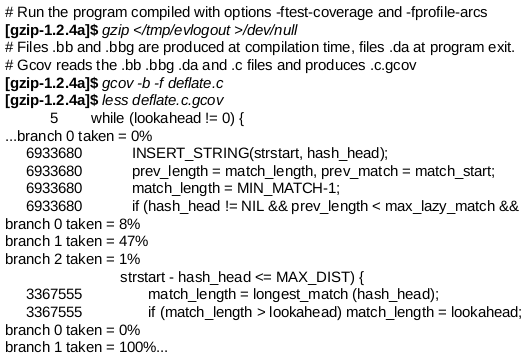
\includegraphics[width = 7cm]{gcov_results.png}
\caption{résultats typique gcov}
\label{fig:gcov_results}
\end{figure}

Le surcout en mémoire est d'environ 10 \%. a peu près la même chose pour les données
\section{gprof}
ressemble beaucoup à GCOV. *l'utilisation d'un profileur peut rendre ton programme 2-3 fois plus vite* C'est un profileur qui nous permet de compté chaque entrées dans une fonction encore une fois. Sa nous permet de savoir comment de temps son passer dans chaque fonction. Sa ne fait pas exactement la même chose que GCOV, sa fait une répartition dans le temps d'utilisation de nos fonctions, sa regarde à chaque x temps dans quel fonction nous somme rendus, et sa fait une stats avec sa. sa compte combien de fois une fonctions est appelés et aussi de quel place en mémoire.\\

Lorsque le programme compiler va s'exécuter, un timer à chaque 1ms va arrêter le programme, prendre la position du programme (dans quel fonction, de quel addresse la fonction est caller). Sa fait un vecteur de la même size du programme, et dans chaque position sa met le nombre de calls de c'est addresse à fait. \\

par contre, vu que sa s'exécute seulement à chaque 1ms, on peut généralement pas capter la routine d'initialisation. \\

Sa alloue un très grand espaces mémoire, mais c'est très utiles et sa coute pas beaucoup dépendamment de la fréquence de sampling (1ms vs 1us vs 5ms).\\

Pour résumer, sa illustre quand même très bien le temps passer dans chaque fonctions. Sa fait un arbre qui montre l'utilisation de chaque fonction (voir TP1).\\

l'attribution proportiel en temps d'appel implique que tout les appels sont identique, ce qui n'est pas si vraie que sa.. certaines parties du programme fait des write qui peut varier en temps dépendamment de l'espace ou un écris, gprof ne peut pas vraiment comprendre ces subtilités.\\

\begin{figure}[!ht]
\centering
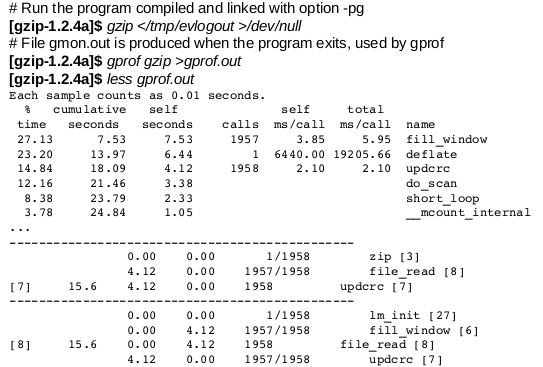
\includegraphics[width = 7cm]{gprof.png}
\caption{Exemple Gprof}
\label{fig:gprof}
\end{figure}

On peut voir que file\_read ne consomme pas beaucoup de cpu, mais qu'il prend quand même beaucoup de temps dans updcrc. Sa permet de voir ou on passe notre temps\\

GPROF nous donne le choix avec les options de compilations de faire pas mal ce qu'on veut avec une précision variable.

\section{Oprofile}
Outil de profilage qui fait uniquement la partie d'échantillonage (il prend juste le temps, pas l'arbre d'exécutions). sur Linux, Perf fait pas mal la même chose. l'idée c'est comme gprof, sauf qu'on utilise les compteurs de performances (on trigger à chaque 100k fautes de caches.. etc). C'est très flexible.\\

On peut demander qu'à chaque fautes il y a une interruption, sa compte, sa nous donne une idées des pertes CPU causés par nos erreurs. \\

\begin{figure}[!ht]
\centering
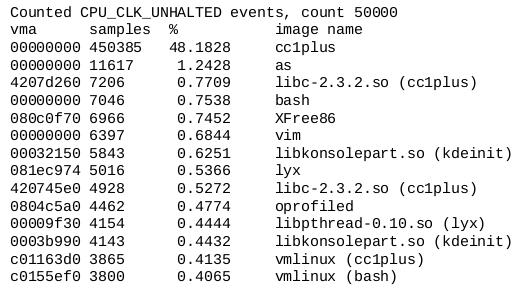
\includegraphics[width = 7cm]{oprofile.png}
\caption{Exemple d'Oprofile}
\label{fig:oprofile}
\end{figure}

on peut voir que cc1plus à été interrompu 50\% du temps, sa veut dire qu'elle a causé la moitié des fautes de caches.\\

on peut même demander d'annoter le code sources en assembleur, en mettant le compte de chaque fonction.\\

\begin{figure}[!ht]
\centering
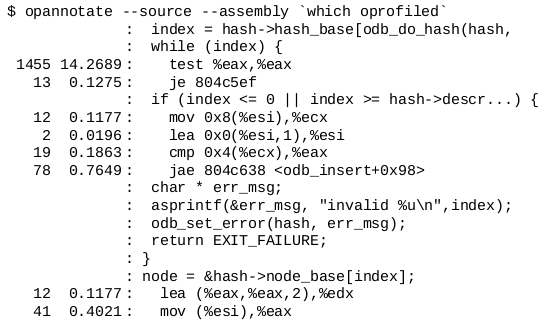
\includegraphics[width = 7cm]{oprofile_assembleur.png}
\caption{Exemple d'Oprofile avec assembeur}
\label{fig:oprofile_assembly}
\end{figure}

Les dernier outils qu'on a vu date de quand même très longtemps, il existait des variantes mais c'est pas mal les classiques

\section{Valgrind}
Valgrind est un peu plus spécialisé. Plusieurs problèmes comme les course, les fautes de caches, et autres erreurs beaucoup spécialisé sont difficile débugger avec les vieux outils. l'environnement Valgrind décompile le code, et peut ajouter de l'instrumentation a plusieurs endroit, recompiler, et exécuter normalement avec des compteurs. \\

\subsection{Memcheck}
Un outil d'instrumentation qui permet de voir chaque écriture et lecture en mémoire, de même que malloc/free sont instrumentés. \\

Sa aloue un grand vecteurs qui compte pour chaque case mémoire si c'est allouer, utiliser, et autres.. Sa regarde toutes les bitfields (très fins).\\

évidemment, sa double la mémoire requis, sauf que sa aide beaucoup.\\

en faisant un malloc, sa déclare la zone accessible (sa change le vecteurs) et sa fait d'autres modif.\\

En faisant un écriture, on regarde dans le vecteurs si c'est accessible. Sa nous donne une assurance qu'on n'a pas de corruption mémoire. Par compte, sa rend notre programme de 10 à 30 fois plus lent.\\

sa détecte: 
\begin{itemize}
\item les accès invalides
\item l'utilisation de bits ou octets non initialisés
\item les fuites de mémoire 
\item les free redondants ou incorrects 
\item les recoupement d'adresse source et destination pour les fonctions de la famille de memcpy.
\end{itemize}

C'est un outil très efficace pour les programme qui peut rouler 10-30 plus lent, genre pas les trucs real-time / embarqué.

\subsection{cachegrind}
Un outil a priori moins intéressant. Sa instrument les accès mémoire. Il va à chaque accès voir ou sa se situe en cache (soit spécifier ou découvert automatiquement la longueur de cache). Sa comprend un peu le comportement expecté en cache, il peut ensuite fournir de l'information sur le programme pour dire si il y a des problèmes ou non. Si on a accès a un profileur, sa sert pas à grand chose.. Un point positifs, c'est que c'est indépendant de l'architecture, alors on peux tester sur des trucs assez ésotérique.\\

Il y a l'option callgrind, qui est utiliser un peu plus souvent (c'est comme gprof) sa donne l'arbre d'utilisation de chaque fonction ainsi que l'adresse ou on l'a caller. sa regarde les appellants jusqu'a n niveau (spécifié).  \\

sa prend environ 50x plus de temps.\\

Par contre, il est beaucoup plus précis que gprof.
\subsection{Address Sanitizer}
Version de google de memcheck, sa instrument à la compilation.. etc. pareil comme memcheck. Sa implique qu'ils ont une version source de toutes leurs applications. (ils roulent linux.. alors c'est chill).\\

pour chaque blocs de 8 octets, ils checkent si la mémoire est allouer au lieu de chaque bits. on perd alors notre accès au bitfields sauf que sa rend notre programme beaucoup plus performant (sa réduit l'overhead)\\

On peut changer aussi la résolution (16 bits, 32 bits, 64 bits...) tout se fait par morceaux, alors sa se gère quand même mieux qu'une size batard.\\

Pour le reste, sa regarde quand même les chose similaires à memcheck, sauf que sa roule 2 fois plus lent au lieu de 10-30 fois.. c'est mieux pour le real-time.\\

Un espace libre est alloué eentre les espaces, sa fait une zone de quarantaine pour un certain temps et sa nous permet de voir des chose assez intéressantes..\\

watchpoint dans le déboggeur pour les cas difficile, en mettant un seul watchpoint, il n'y a pas encore beaucoup de ralentissement. Par contre, en mettant trois watchpoint, sa devient très lent. C'est du au nombre de registre disponible dans ton CPU. sa fait des contexte switch à tout les deux isntruction assembleur alors sa fait du MÉGA-overhead.\\

en mettant un watchpoint, sa nous permet d'observer des addresse mémoire ou il y a rien, on les met avant nos structure pour voir quand la corruption se passe

\subsection{Massif}
c'est comme la même chose que Heap Profile (voir plus bas). Sa regarde l'arbre d'appel des fonctions d'allocations et libération de mémoire, sa fait ensuite un arbre qui montre quel fonction appel malloc et free et regarde la quantité de mémoire utilisé / temps de processeur utilisé

\subsection{Helgrind}
Helgrind est encore plus spécialiser, sa nous permet d'instrumenté les programmes en mémoire partager. Sa détecte les course.. Sa détecte les erreur bizarre qui érrone mes données. Sa nous permet de trouver les problème plus difficile sur les applications parallèles. On peut aussi faire la vérification formel(lol)\\

Chaque variable en mémoire est dans l'état exclusif possédés par le segment de fil qui l'a accédées. Si un autre essaie de l'accéd et que c'est disjoint, le nouveau segment devient propriétaire. Sa analyse le processus de synchronisation des caches (MESI et MOESI) et sa peut nous dire ou sont les problèmes.\\

Sa fait aussi beaucoup d'analyse sur les verrous. pour chaque verrous il y une variable, il ne sait pas quel variable est accédés a quel verrous, sa regarde les accès mémoire et elle essaie d'associer les verrous aux variable. Quand il pense qu'il a une association, il regarde si l'accès à la mémoire se fait en respectant le verrous, lorsqu'il a un hit, il l'affiche.\\

Sa ralentit beaucoup le programme (genre 100x)\\

\begin{figure}[!ht]
\centering
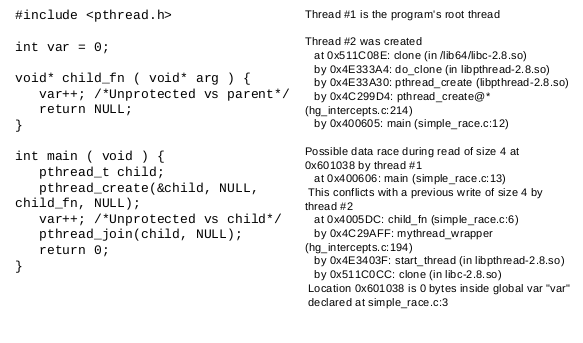
\includegraphics[width = 7cm]{detection_course.png}
\caption{Exemple de détection des course d'Helgrind}
\label{fig:detection_course}
\end{figure}

Helgrind va aller plus loin que l'intersection des verrous. Il peut aussi voir les deadlocks.\\

Il peut détecter à l'avance les problèmes de deadlocks, il fait une verification par tread/verrous. C'est quand même couteux. Il regarde l'ordre de prise des verrous et batis un graphe dirigié avec des contraintes. Il dit quel verrous devrait être pris avant quel autre de sorte que le programme ne se met pas dans un deadlocks. \\

\begin{figure}[!ht]
\centering
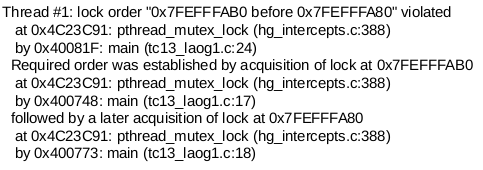
\includegraphics[width = 7cm]{ordre_verrous.png}
\caption{Ordre des verrous}
\label{fig:ordre_verrous}
\end{figure}

\section{Lockdep}
C'est un autre outil qui vérifie l'ordre de prise des verrous. C'est un peu plus lent, mais sa fait la même vérif. qu'avec Helgrind. Sa fait un graphe de prise d'ordre et mets des contraintes (par threads). Et sa fait aussi une vérification du niveau et contexte dans lequel est pris une classe de verrous. normal, irq, irq actifs ou non. Un verrou pris en
mode normal avec irq actifs et aussi en mode irq peut mener à
un bloquage.\\

c'est une convention de règle de priorité, on regarde si on respecte des règles spécifique pour l'utilisation de verrous. C'est très utiles pour le développement des drivers.\\

\section{Thread Sanitizer}

C'est un outil développer par Google. C'est thread safe, comparément à valgrind..\\

l'app. prend 5 à 10 fois plus de mémoire avec 2 à 20 fois plus de temps.\\

Sa instrumente à la compilation toute les lectures et ecriture en mémoire, sa regarde si chaque accès respecte la synchronisation.. Sa crée des cases par mots pour stocker l'info (si c'est accessible, si c'est utiliser..).. Sa conserve aussi un tampon des derniers appels, et retours sur chaque fil d'exécution de manière qui puisse découvrire les cas de conflits.\\

\section{CPU profile}
Un autre outil de google. qui cherche a faire la même chose que gprof en terme d'échantillonnage, par contre, ils echantillones la pile au complet comme valgrind. Il peuvent rebatire une pile d'appel parfait et peuvent recréer presque parfaitement l'exécution basé sur la pile (à chaque 1, 5 ms). ce qui nous manque c'est les fonction d'init, pas contre c'est négligeable.\\

Normalement, la pile d'appel à a peu près 10-15 pile d'appel. Sa peut varier si on se sert un peu trop de l'orienté objet (genre 50?)\\

Un programme performance typique à a peu près 15.\\

Par contre, en terme de couts c'est beaucoup mieux. Au cout du fait qu'il n'y a pas un compte exact comme avec gpof.

\section{Heap Profile}
Sa analyse les même chose que le CPU Profile, sauf que c'Est spécialifer pour les procédure d'attribution de mémoire (malloc, free, etc.). sa regarde la collection de garbage, ainsi que le temps mis à initialiser nos données. Chaque allocation ou libération en mémoire est prise en compte par l'outil et est échantillonné, ensuite sa analyse l'arbre d'appel pour ces fonctions ainsi que l'espace prise par toutes ces fonctions.\\

Sa regarde quel fonctions fait quel allocations de mémoire, sa regarde d'ou vient les problèmes de leak mémoire et autres. Sa fonction avec C, et avec Go

\section{Traces d'exécution multi-coeurs}
Les outils qu'on vient de voir résous des problèmes très spécifiques. Pour les problème d'ordre générale, on se sert d'un déboggeur. Pour un outil générique qui n'est pas un déboggeur, on utilise un outil de tracage et on analyse la trace a posteriori. Ces outils sont utils pour des problème qui sont un peut trop subtiles pour le déboggeur.\\

Sur linux:
\begin{itemize}
\item LTTng : développer à Poly, dans le lab du prof.
\item dTrace : Développer par Oracle.
\item Red Hat System Tap : similaire à dTrace, mais pour Red Hat
\item Ftrace et Perf : outil de bas niveau qui fait partie des outils par défauts de linux. Sa reprend certains élément des contributions de LTTng au noyau linux.
\item GDB tracepoint : nouvelle fonction permettant de placer efficacement des points de trace dans les applications à partir du déboggeur. Sa nous permet de débogger les problèmes en temps-réel. 
\item DynInst: outil pour l'insertion dynamique de points de trace dans des exécutables avant ou pendant leur exécution. sa décompile, ajoute les points de traces, recompile, et sa fait des logs. c'est très couteux/ invasif 
\end{itemize}

l'idée c'est qu'on ne sait jamais le problème d'avance. Alors on insère certains point de traces dans notre programme qui sont stratégique et nous permet de faire beaucoup de déduction. Au moment de l'exécution, on active les points de traces statique/dynamique et quand on spécifie quel outil on appel lorsqu'on frape un point de trace. \textbf{eBPF} nous permet de configurer des règles d'avance et eBPF va gérer les points de traces. Sa convertit en bytecode qui est ensuite converti en exécutables.\\

Avec sa, lorsqu'on rencontre un point de trace, sa nous permet de faire un peu ce qu'on veut (spécifier dans eBPF).\\

Normalement, on écrit dans un tampon en mémoire. lorsqu'on a un problème, on prend une copie du tampon et on l'envoie dans un fichier pour analyse. (comme une black box).\\

On a aussi la possibilité d'ajouter des conditions qui peut convertir du C en bytecode eBPF, sa nous permet d'associer des conditions en points de trace qui est dynamiquement associer aux variables.. Sa nous permet de gérer le surcout/ quantité de données.\\

l'événement va être écris dans le tampon avec un timestamp, qui nous permet de recréer un événement. \\

Sa nous donne vraiment une grande flexibilité sur qu'est-ce qu'on veut avoir et comment, toute en gardant la possibilité de faire des compromis de performances. Ce qui est pas toujours le cas pour les autres outils de tracages.\\

\begin{figure}[!ht]
\centering
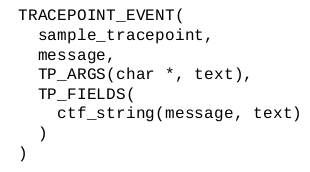
\includegraphics[width = 7cm]{definition_trace.png}
\caption{Définition d'une trace}
\end{figure}
les gens fonts souvent une sorte d'équivalent en printf. c'est à dire, lorsqu,on rencontre la condition, on appel une fonction avec plein de printf qui imprime un peut ce qui se passe présentement. Par contre, c'est dure d'être cohérent.\\

Un des problèmes est un peut la conformité, ce nest pas tous les outils qui utilise le même format.

\subsection{Utilisation de LTTng}
En exécutant un programme, on peut spécifier les points de traces qu'on veut regarder. On fait sa en créant une session de tracage qui gère par lui-même ses fichiers d'analyse. En le fermant, on peut quand même avoir accès au fichier pour pouvoir analyser. \\

\begin{figure}[!ht]
\centering
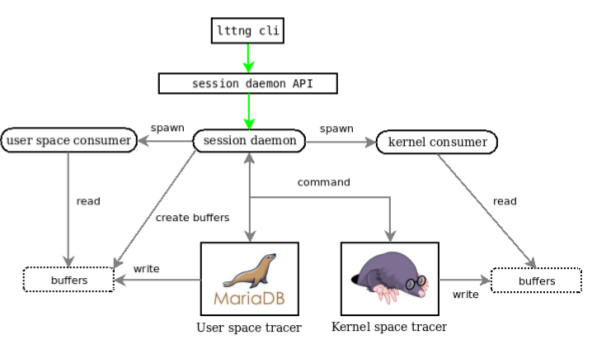
\includegraphics[width = 7cm]{trace_simultane.png}
\caption{Trace Simultané}
\end{figure}
le client ouvre des pipes avec le daemon..\\

\begin{figure}[!ht]
\centering
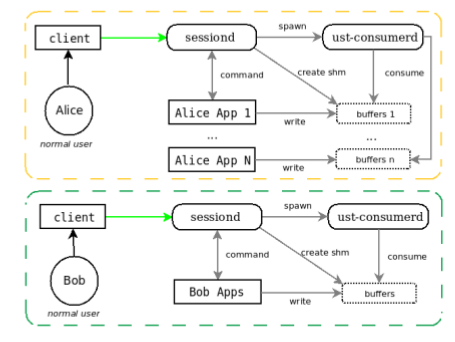
\includegraphics[width = 7cm]{session_usager_different.png}
\caption{Session d'usagers différents}
\end{figure}



les images explique visuellement le fonction de l'outil LTTng.\\

\subsection{Pourquoi une trace avec un cout minimale?}
\begin{figure}
\centering
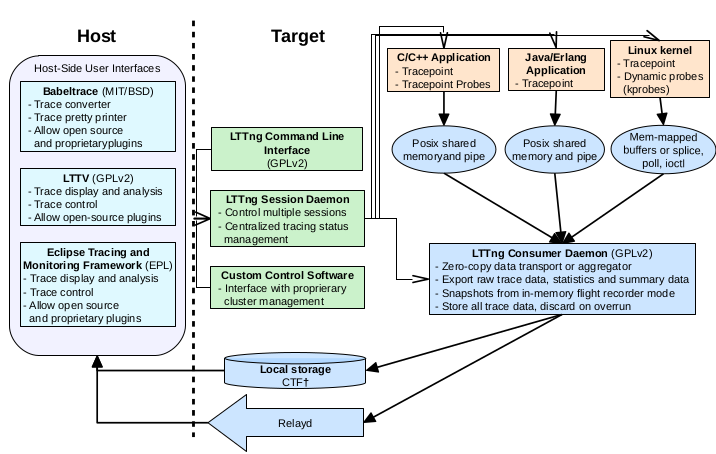
\includegraphics[width = 7cm]{low_overhead.png}
\caption{Gestion de LTTNG}
\end{figure}

strace trace toutes les appels système, sauf que sa ralenti proportionellement en fonction du nombre d'appel système. C'est ce qu'on voulait.. pas de bug.. \\

\begin{figure}[!ht]
\centering
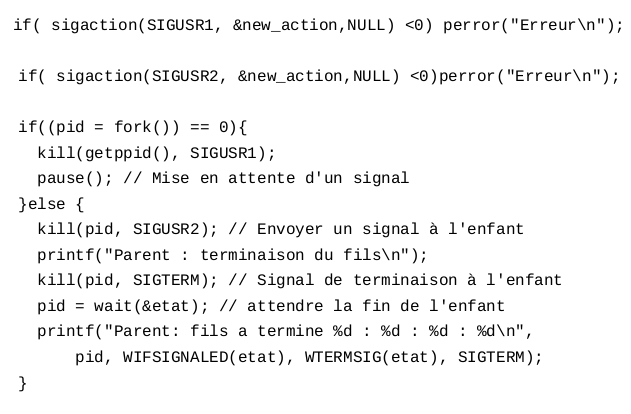
\includegraphics[width = 7cm]{strace_code.png}
\caption{bug dans la prise de trace sans cout minimale}
\end{figure}

\begin{figure}[!ht]
\centering
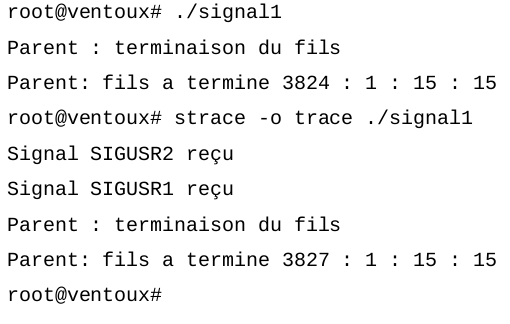
\includegraphics[width = 7cm]{strace.png}
\caption{Il n'y a pas de bug en faisant sa..}
\end{figure}
Par contre, lorsqu'on utilise un traceur (lttng), on peut voir que le bug est encore la (?bug?) le problème a été capté sur la trace. Le problème est du au fait que l'enfant n'a pas eu le temps d'envoyer sigusr 1 avant que l'appel de la mère s'est fait. c'est un exemple typique d'une course.\\

La performance est important, en utilisant un outil lent, on aurait jamais pu voir qu'un course se produirait\\

\begin{figure}[!ht]
\centering
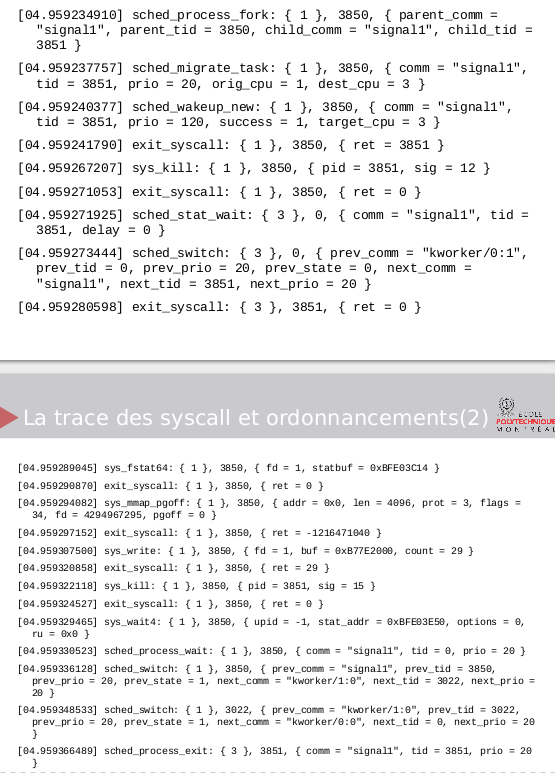
\includegraphics[width = 6cm]{strace_performance.png}
\caption{la trace des syscalls}
\end{figure}

\subsection{Exemple d'optimisation}
Certaines optimisation ont été faite en espace usager, sans aucun interaction ave le système d'exploitation. Exemple, en mettant l'activation d'un point de trace sur un if improbable, sa va arriver, mais pas toujours, alors le cout est quand même bas. \\

En utilisant un format binaire natif. Normalisé en tant que \textbf{Multi-core association common trace format.}\\

en utilisant  tampons par CPU avec opérations sans verrous. \\

technique de synchro entre la lecture des infos de config ainsi que leur modif par la technique Read Copy Update (RCU)\\

Aucune copie en mémoire directement..
\section{Autres}
l'analyse d'un trace se fait en listant les événements de différentes traces en utiilisant une référence de temps commune (synchro a posteriori). On construit ensuite un modèle du système en prenant les infos de traces pour fournir de l'info sur ce que le système fait(appels systèmes, lecture/ ecriture de fichier.. etc). Avec une navigation efficace sur l'info, sa fait des analyse quand même assez efficace.\\

\subsection{synchronisation de traces}
Chaque noeud à une horloge indépendante, alors même les timestamps ne peuvent pas nécessairement donnée une bonne synchronisation (sur plusieurs CPU). Sa fait une différence de première ordre : valeur initiale, fréquence différentes. c'est possible d'avoir des compteurs logiciels qui sont très forts, sauf que sa prend un peu de performance. La majorité des différences sont causé par la différence de fréquences des crystaux.\\

On peut voir aussi un effet de second ordre avec la variabilité de l'ordre ainsi que la latence de lecture de l'horloge, vu que c'est dérivé de la fréquence dans le temps (par exemple, la température, l'humidité et la tension des dispositif d'hydro-québec).\\

Le principes est d'identifier les envois et réceptions corresponants pour les paquets envoyés sur le réseau et utiliser l'information du paquet pour estimer les coéfficient de l'horloge A vs. l'horloge B.\\

\begin{figure}[!ht]
\centering
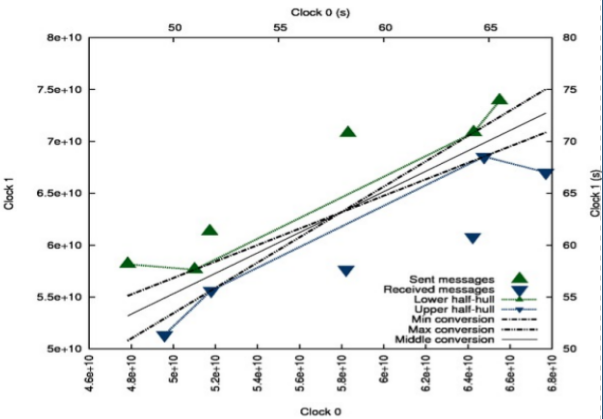
\includegraphics[width = 7cm]{convex_hull.png}
\caption{Graphe de performance des horloges}
\end{figure}

C'est un processus qui nous permet de voir le temps d'aller retour entre les deux ordis, ce qui nous aide a les synchroniser.\\

Avec sa, on peut modéliser l'accès ressources en XML avec les différents événements (type, valeurs des champs) et des changement d'états qu'ils causent. On peut voir quel thread est sur quel coeur, quel device est ouvert.. On peut reconstruire presque toutes les structure de données sur le système d'exploitation. On peut en faire un arbre/ base de données\\

\begin{figure}[!ht]
\centering
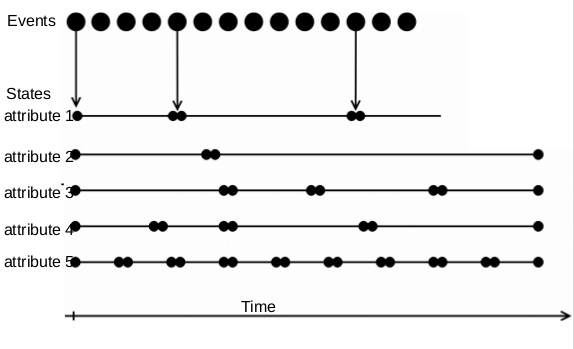
\includegraphics[width = 7cm]{modelisation_etat.png}
\caption{Modélisation de l'état}
\end{figure}
Sa représente l'état courant un moment données. Lors de la modélisation, on peut faire des liens entres les différents états et ainsi en faire nos déductions. \\

\begin{figure}[!ht]
\centering
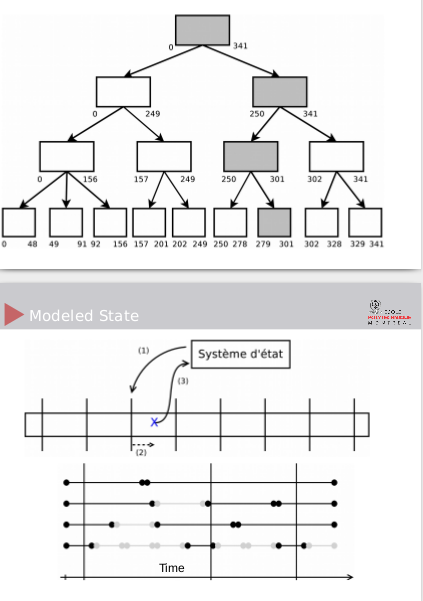
\includegraphics[width = 7cm]{53_55.png}
\caption{Historique et état modélisé}
\end{figure}
\subsection{Analyse du chemin critique}
Le principe est d'analyser, pour chaque processus, quel états est le bottleneck en terme de vitesse. on trouve les points qui nous ralenti, et ensuite on regarde pourquoi. On peut ensuite faire nos modifications si c'est possible, et essayer de miniser les pertes causer par notre chemins critiques.\\

on essaierait de miniser le nombre de requêtes. Au début, on se demandait si apt-get était capable d'être optimiser avec le chemin critique. On a trouver que apt-get faisait juste attendre et assumait qu'après 0.5 secondes c'était fini (on perd beaucoup de temps quand c'est fini).\\

On peut aussi regrouper les tâches en métriques, comme par exemple le write qui peut prendre un temps indéterminer en fonction du matériel sur lequel on écrit\\

\begin{figure}[!ht]
\centering
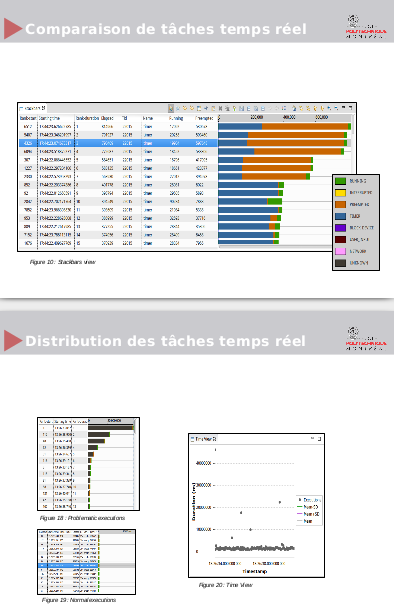
\includegraphics[width = 7cm]{59-60.png}
\caption{résultats des métriques}
\end{figure}
On peut aussi visualiser les différence entre les groupes. \\

\begin{figure}[!ht]
\centering
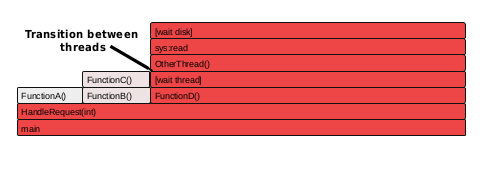
\includegraphics[width = 7cm]{62.png}
\caption{différences entre les groupes}
\end{figure}
\section{Vtune}
Un outil offert sur Linux et Windows. Sa fait du profilage par minuterie ou compteur (Valgrind?, gProf?) sa montre l'état du fil d'exécution en fonction du temps, sa montre le montant d'attente active et passive par verrou ou section critique. Il y a même un API pour pouvoir mettre dans des programme qui vont faire exécuter des événements pour Vtune a fin d'analyse.\\

\section{Windows Performance Toolkit}
Instrumention du noyau et des librairies système avec Event Tracing for Windows(ETW). \\

C'est un outils qui offre la possibilité d'ajouter des points de traces dans des applications et de pouvoir les activer dynamiquement. Les traces peuvent ensuite être analyser avec des outils graphique.. Par contre, la trace doit être analyser sur l'ordinateur dont la trace a été effectué.


\section{Vampir}
*Les européens sont trop sophistiqués..* \\

C'est un outil développé en Allemagne, le but de l'outil est d'analyser la performance des programme fonctionnant sur plusieurs différents processeurs. On peut voir les événement en fonction du temps/ autres métrique par arbre d'appels (comme gprof). Pour résumer, sa analyse les programmes fait avec MPI et autres librairies de parallelisme distribués. On peut définir nos métriques d'évaluations et tout le kit, sa fonctionne avec le Open Trace Format..

\section{PARAver}
Un outil de visualisation des événements/performance pour applications paralleles. C'est développer au centre national de supercomputing de Barcelone. Par contre, il faut donné plein d'info pour téléchargé malgré le statut open source. C'est un peu louche... \\

Le but de paraver est très similaire à Vampir, c'est un outil de visualisation pour le systèmes paralleles. C'est entièrement adaptable à différents types de traces. Il est possible d'ajouter des modules supplémentaires et même de comparer des traces. (sa ressemble à motif??)
\section{Tuning Analysis Utilities}
C'est américain, projet de l'université d'Oregon. Sa fait de l'instrumentation par interposition de librairie. (LDPreload). Sa test les différentes version de librairies. Sa embale les fonctions MPI ordinaire. Analysis statique du code source pour l'insertion automatique d'instrumentation.\\

On peut faire une activation sélective des points de trace. On a aussi une utilisation de minuterie ou de compteur matériels pour obtenir un profil (Paraprof).\\

On a aussi jumpshot pour voir l'état des fils d'exécution en fonction du temps.\\

Interface graphique très primitive aussi...

\section{CODEXL}
Outil d'AMD. il y en a un qui sert à développer des jeux, et un pour développer du OpenCL. On peut voir l'arbre d'appel et les transfert de données OpenCL (carte graphique).  La plus grande difficulté est qu'on ne peut pas directement faire une trace sur la carte graphique. Le kernel OpenCL doit être loader avec des flags pour qu'il envoit des message sur la trace CPU. L'outil s'en occupe.\\

fait notable: CodeXL fait une chaine d'outil completement opensource. On peut vraiment voir le fonctionnement
\section{APITrace}
Trace les appels OpenGL (graphique). l'idée de l'outil est d'avoir les information sur la cartes graphique frame par frames. Sa nous permet de voir l'arbre d'appel et certain bug soit dans le programme ou la librairie OpenGL.
\section{GPUView}
Trace des événement noyau et en particulier de toutes les commandes du sous-systèmes.
\section{Promela et SPIN}
Vérification formel. l'idée est d'être capable de démontré que dans tout les cas notre programme va donner le bon résultats (course). Sa regarde le fonctionnement de tout les mutex, barrière et autres. \\

il faut être capable d'exprimer les différents processus concurrents. Si on a trois threads avec leur propre instruction, on essaye toutes les combinaisons possibles (presque) pour pouvoir s'assurer qu'on respecte toujours les paramètre données ou bien pour tout simplement juste voir les résultats possible.\\ 

\begin{figure}[!ht]
\centering
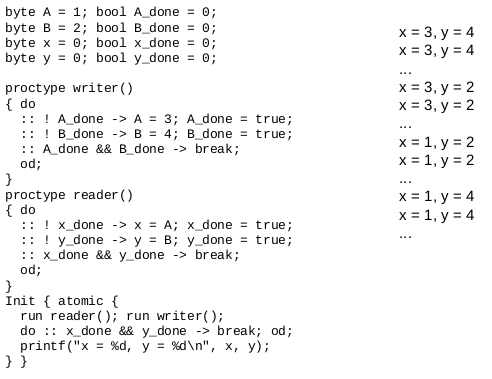
\includegraphics[width = 7cm]{promela.png}
\caption{exemple de Promela}
\end{figure}

Le prof utilise le tracage, pour les chose spécifique = profilage avec perf pour des problèmes performance, pour mémoire gprof. Peut-être Valgrind si la performance n'est pas trop important. Pour des problemes avec MPI, utiliser TAU
\section{OpenSpeedShop}

https://openspeedshop.org

Les fonctionalités d'openspeeshop sont tous des choses que nous avons vu jusqu'à présent. Ils sont tous intégrés dans un seul outils et comporte même certains outils perfomance GPU. Ils fournissent les acétates pour un tutorial de leur outils, c'est assez complet (environ 100 slides). Ils sont entrain tranquilement d'amasser une communauté asser intéressante. Ils sont mieux financer et on la collaboration de plusieurs groupes.\\

Ils ont une approche moderne (QT) et sa fonctionne quand même bien. C'est quand même modulaire, alors c'est très customizable (les gens OpenSource aime sa). \\

Sa va surement continuer à se développer dans les prochaines années.
\chapter{Virtualisation Haute Performance}
au niveau de l'infrastructure physique:
\begin{itemize}
\item a l'épreuve des tremblements de terres
\item un peu en élévation
\item pas beaucoup de fenêtres
\item Centre dans des conteneurs, permet le déplacement et amène de la flexibilité
\item Bâtiment rudimentaire avec ventilation extérieur pour avoir des couts minimes, sa permet un bon déplacement d'air et sa fait que sa ne vient jamais trop chaud à l'intérieur
\item grande puissance d'alimentation électrique
\item Refroidissement à l'eau et à l'air. Pays froid (Canada, pays nordique)
\end{itemize}
Climatisaton:
\begin{itemize}
\item Chaque Watt consommé utilise 1 W pour le calcule plus 1 W pour climatiser (beaucoup de puissance)
\item Air forcé à travers le chassis, watercooling block
\item Compromis entre température et usure du matériel
\item utiliser l'air extérieur, accepter une température plus haute et économiser pour réacheter du matériel lorsque sa plante..
\item Environnement sans humain non éclairé
\end{itemize}

On fait sa par secteur pour chaque ordinateur. On passe du 110V $\rightarrow$ 12V DC $\rightarrow$ 110V jusque dans nos power bars. On utilise souvent aussi une pile de secours/génératrice. \\

On regarde aussi beaucoup la performance de flop/watt, c'est plus écologique.\\

En terme de chassis (les boites) on utilise souvent des boitiers 1U ou 3U (U = 3.7 pouces). On organise sa en rack, on a des standard pour rendre sa compacte:\\

On met les carte à la verticale, on les met au .75 pouces, on les mets à la verticale pour que ll'air puisse monter et optimiser le transfert de chaleur. On peut facilement se rendre à un grand nombre de carte. On joue aussi beaucoup avec la profondeur des chassis pour optimiser l'espace et le flot d'air dans la structure. Sa prend quand même un moyen de refroidissement.\\

La compagnie Facebook à voulu faire les choses efficacement sans tout faire sur mesure pour réduire les couts. Ils ont mis une organisation en place appelé OpenHardware qui nous permet de faire du stocke pour facebook, Openhardware met leur plans en ligne et one peut faire leur stocks pour eux en échange d'une compensation. Ultimement, ils cherchent à descendre le cout du matériel en le sourcant directement au producteurs.\\

Réseautique:\\

Il faut de la réseautique spécialisé à faible latence, le plus de latence, le plus de temps passer à attendre = le plus de perte de calculs..\\

On peut se servir aussi de réseaux ordinaire (10G), mais c'est pas trop great.. C'est mieux d'aller chez Infiniband pour avoir la performance. Il faut aussi prendre en considération la connection entre les différents noeuds, on peut avoir toutes les noeuds interconnectés ou bien d'avoir une solution partiellement commutés. On peut choisir d'avoir toute lesnoeuds connectés, mais sa risque de faire un gros clusterf***.\\

\begin{figure}[!ht]
\centering
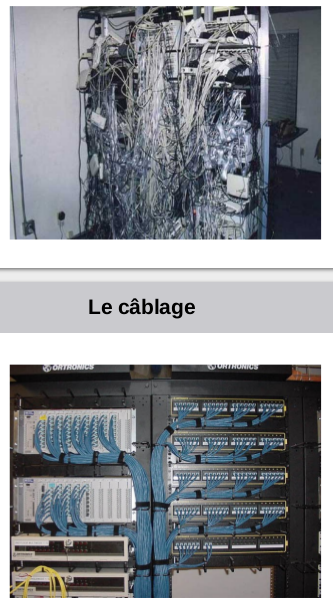
\includegraphics[width = 7cm]{cablage.png}
\caption{Exemple d'un mauvais et bon cablage..}
\end{figure}
\section{Surveillance de système et réseau}
On utilise SNMP pour faire la gestion des noeuds sur le cluster.On peut changer plusieurs paramêtre dans le protocole et sa peut changer les attribut de chaque noeuds dans le cluster. Sa nous permet de faire n'importe quoi avec notre systèmes. Sa prend par contre, une console de gestion qui nous permet d'interroger l'état de chaque noeud sur notre cluster. \\

les console/gestionnaire:
\begin{itemize}
\item Nagios
\item OpenNMS
\item Ganglia
\item IBM Tivoli
\item HP Network
\end{itemize}
Ces console peuvent même faire la découvert automatique du réseaux, sa permet de faire une bonne partie du travail. C'est des commande de l'alimentation et remise à zéro à dstance pour les noeuds par KVM-IP ou BIOS-UEFI, on peut aussi faire de la redirection d'IO sur nos différent noeuds. On peut aussi faire un SSH, mais si la machine est gelé, on doit se servir des méthodes précédentes.\\

Intel a mis un ucontroleur dans la carte réseaux, sa nous permet de faire une communication avec le systèmes gestionnaire et redémarrer la machine en plus de pouvoir changer les paramêtres de BIOS. Par contre, il faut que sa soit sécuritaire, sinon n'importe qui peut avoir l'accès. Les nouveaux chips ont même des systèmes d'exploitation sur les chips eux-mêmes.

\section{Matériel}
Certaines choses doivent être faites pour garder le systèmes opérationels avec un minimum de downtime:
\begin{itemize}
\item Remplacer les disques, blocs d'alimentation ou cartes électroniques assez régulièrement
\item Problèmes subtils causé par du matériel en apparence identique, mais pas complètement compatiable: interférence, chaleur..
\item Contrats de service 4 heur ou 24 heures par jours..
\end{itemize}

Une analogie peut être fait, cattle vs pet.. Cloud = cattle, ou on fait juste changer les défaillance. tandis que le pet on en prend plus soins..\\

Il y a aussi une question d'entretien logiciel: On parle de correction de bug, mais dans les systèmes embarqués, il faut quand même prendre en considération que les producteur de logiciels délaisse leur client précédents il s'en foute, alors on peut être pris avec un bug majeur sans nécessairement avoir d'aide du créateur lui-même. Pour les système critique, c'est mieux d'être conservateur sur la version du systèmes d'exploitation. On cherche vraiment la stabilités tandis que certaines applications cherchent vraiment à avoir du bleeding edge.\\

Tout dépend du contexte..\\

\section{Grappes de Calculs}
Au bout de 5 ans, la valeur résiduelle est près de 0. Il faut vraiment installer les machines le plus vite possible sinon la valeur se perd très rapidement. On finalise l'architecture/processeur à la dernière minute pour vraiment maximiser l'investissement. Il faut aussi considérer l'espace requis (24000 noeuds = grand surface). Il faut aussi s'assurer de pouvoir l'utiliser en tout temps, et de n'importe ou. Normalement, on a une équipe de spécialiste qui sont dédier au bon fonctionnement d'un machine (le plus grand la machine, le plus grand l'équipe).\\

\subsection{Infonuagies}
la virtualisation facilite beaucoup l'implémentation des services sur des plateformes partagés.\\

\subsection{Red Hat MRG}
Red Hat messaging realtime grid. C'étais une architecture d'infonuagies initialement fait pour faire du algorithmic trading. c'est très performants..\\

\subsection{AMPQ}
Protocole d'envoi de mesage pour les applications réparties capable de faible latence. utilisé par Red Hat MRG. pour des applications financière ou militaire avec beaucoup de messages par secondes\\

\begin{figure}[!ht]
\centering
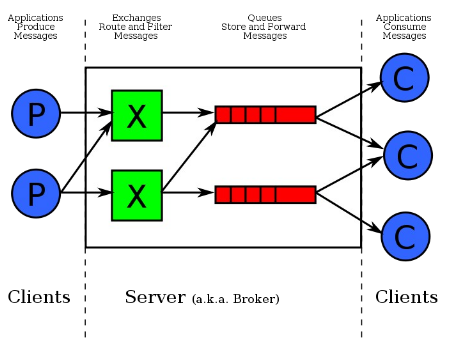
\includegraphics[width = 7cm]{18.png}
\caption{Exemple d'AMPQ}
\end{figure}

C'est fait pour que les messages soit encapsulé et contiennent toute sorte de propriétés comme par exemple l'expiration et tout pleins d'autre choses.. \\


\subsection{Grilles CONDOR}
Condor est un systèmes qui fait la gestion de grille, c-a-d la gestion de noeud à grand échelle.

La grille fait en sorte que la load sur la machine est distribué dans le temps, dépendamment des applications. La notion de grilles n'a pas été utilisé pour très longtemps. C'est revenue chez amazon (EC2). Normalement, pour question de config, toute les machine on un daemon qui dit si cette machine peut accepter des jobs,sont occuper, sont pleins ?\\

Il faut définir les tâches, les noeuds, certains paramêtres de gestions.\\

\begin{figure}[!ht]
\centering
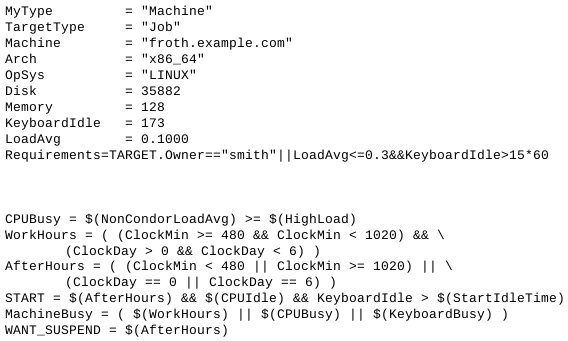
\includegraphics[width = 7cm]{23.png}
\caption{Exemple d'une config}
\end{figure}

il faut spécifier les standard in/out pour voir les résultats.. pleins d'autre choses à faire..\\

Après avoir tout défini en ce qui concerne les tâches, il faut maintenant définir les caractéristique des noeuds. On peut spécifier quel tâches le noeuds peut prendre, quand peuvent-elles les prendre, qui peuvent-elles les prendre, toute ce fait.\\


Une questions délicate : la répartion des ressources. il explique que l'espace est la variable la plus critiques. l'idée est qu'avec une infinité de tâches, comment décider qui à accès à a la machine. Sa prend un système sophistiqués qui défini une hiérarchie qui défini la répartition des calculs sur toutes les utilisateurs.\\

\begin{figure}[!ht]
\centering
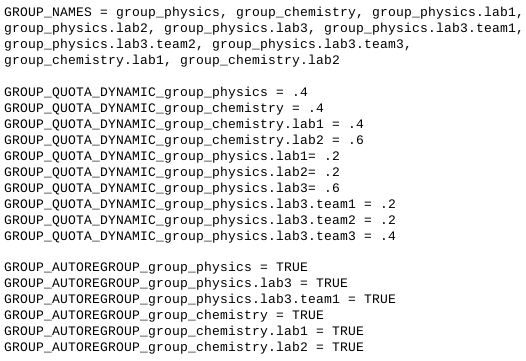
\includegraphics[width = 7cm]{quotas.png}
\caption{Exemple d'un quotas dans une config}
\end{figure}
On peut aussi spécifier d'autre paramêtre subtil comme la consommation d'électricité. On peut décider d'éteindre les machines lorsqu'ils ne sont pas utilisé. On peut aussi spécifier le nombre maximal d'exécution concurrentes qui peuvent s'exécuter. Le monitoring devient un aspect très important dans la gestion du systèmes, on peut avoir une systèmes qui s'assure que tout est respecter, sinon une alarme peut sortir (genre, quand le disque est plein ou qu'on est rendu dans le swap). \\

Condor est aussi à l'épreuve des pannes, il écrit régulièrement dans un fichier expliquant qu'est-ce qui se passe et lorsqu'il y a une panne, il fait un reboot et ensuite reprend son travail ou il avait arreter.\\

\subsubsection{Dagman}
dagman offre la possibilités de spécifier des groupes de tâche interreliés dans un graphe. On peut mêmes imbriqués ces graphes pour avoir des groupes de tâches très complexe, et ensuite pouvoir spécifier des variables pour ces groupes de tâches.\\

Globalement, MRG est un système open source qui offre les mêmes foncitonnalités les un les autres. Leur buts est des faire la gestion de clouds
\section{Virtualisation}
On fait la virtualisation parce que ce n'est pas tout le monde qui ont les moyens d'installer des mega systèmes. Sa nous permet de louer des instances de machines offert sur differt plateforme (amazon) et qui permet la facilité a installer les services sur leur machines.\\

Wine : librairie qui roule les librairies windows sur linux.. par contre, il y a des fois ou sa ne marchent pas du tout.. Sa ne marche presque jamais sur les jeux (20\%). Il faut être près a ajouter des librairies sur Wine, et on peut sa casser la tête.\\

Si on utilise pas Wine, c'est bien de pouvoir virtualiser nos services pour qu'ils puissent rouler sur n'importe quel systèmes d'exploitation.\\

\subsection{conteneurs}
systèmes ou un seul noyau avec des espaces de noms séparés par conteneur pour les PID, IPC, usagers, réseaxu, /proc, hostmname, fichiers.. etc.\\

Chaque conteneurs peut rouler une version différentes des librairiesm applications.. mais il n'y a qu'un seul noyau en exécution. chaque conteneurs est utilisé par un usagers. Cette solution n'implique aucun cout en performance, sauf la mémoire non partagée par les version différentes (exemple, librairie C), si c'est le cas.\\

Voici des exemples:\\
\begin{itemize}
\item Linux LXC
\item FreeBSD Jails
\item Solaris containers
\end{itemize}

\subsection{Simulateurs d'exécution}
Si les conteneurs ne fonctionnent pas, on peut se servir de simulatuer d'exécution. C'est une programme qui simule l'exécution une par une de ton programme. On peut pré-traduire les instructions d'une architecture à l'autre, mais en générale, c'est optimiser pour la recompilation dynamique.. sa peut être de 5 à 50 fois plus lent. On est aussi à risque de bug, car il y a quelques différences entre le fonctionnement des systèmes exploitation (exemple: mode protéger génère des interruptions sur windows).\\

\begin{itemize}
\item 2: remplacement de certaines instruction
\item 5: recompilation dynamique
\item 50: interprétation
\end{itemize}

On ne veut généralement pas s'en servir, sauf que pour déveloper des apps cellulaires, sa peut être utile
\subsection{Intel VT, AMD V (virtualisation matériel)}
équivalent d'une interruption sauf qu'on associe un contexte à l'environnement. Sa devient problèmatique lorsqu'on essaie d'avoir un accès au ssytème d'exploitation et aux périphériques. C'est problématique car il faut émuler les accès disques.. c'est très lents, c'est la ou on va être ralenti considérablement. \\

PCI Passthrough --\\

on a pratique la même vitesse, jusqu'à peut-être deux fois plus lent.. Si on a un genre de micro-benchmark avec beaucoup d'accès système/IO, sa risque d'être beaucoup plus lent.\\

le principe est que le OS en virtuel ce fait donnée un plage mémoire (ex, il demande 4G), et quand il parle directement au noyau, il exécute toujours dans le 4g, cependant, le OS lui fait la traduction du 0- 4g jusqu'à la vraie addresse physique en mémoire. toute le mapping mémoire dans le OS virtuel doit être émulé dans le OS natif, tout ce travail d'émulation de table de pages doit être fait au deux endroit, alors lorsqu'on fait beaucoup d'opérations de gestion de mémoire, le overhead grandit. Sa fait en sorte qu'on a plusieurs différents étages de table de pages. On peut voir des ralentissement d'environ 20\% dépendamment de l'utilisation\\
\begin{itemize}
\item 2-3 \% : Pas de mise à jour
\item 50\% : beaucoup de gestion mémoire
\item 600\% : Micro-benchmark
\end{itemize}

Les machines virtuels sont rendu efficaces, par contre, il y a quand même des problèmes. La virtualisation se fait bien au premier niveau, par contre, quand on va au deuxième niveau, sa devient vraiment raide.\\

\subsection{Paravirtualisation}
entre les deux. une collaboration entre une virtualisation matérielle et logiciel. c'est comme un deuxième niveau d'appel systèmes. Il y a un mecanisme qui ressemble au appels systèmes. C'est utilisé par Xen, VMWare le permet aussi en plus d'OpenBox. KVM peut soit utiliser le matériel de virtualisation ou la paravirtualisation si disponible. Le boot d'une machine virtuel sur linux se fait automatiquement (il voit si c'est une machine virtuel) Les pointeurs aux fonctions sont changer aux version virtuelles (paravirtualisation). Il prend en compte si c'est sur une machine native ou virtuelle et optimise en conséquence.\\

on se retrouve avec un solution, dépendamment de plusieurs chose, qui risque d'être plus performant. par contre, il faut installer une suite de driver spécialiser pour la paravirtualisation.
\subsection{Hyperviseur}
Très populaire. (Xen) amazon roulait Xen jusqu'à tout récemment (maintenant KVM). c'est un système d'exploitation minimale qui gère les interruptions et les accès aux périphériques afin de les répartir entre les systèmes d'exploitation des machines virtuelles. Sa gère les interruption et la mémoire.\\

Évidemment, on ne voulait pas réimplmenter tout les drivers. On a mit le domaine 0 à linux (qui gère), et les autres domaines seront les autres services qu'on roule sur nos machines. \\

Certain soucit sont apparus, le controle d'interruption est devenue très compliqué. Si on a plusieurs coeurs, c'etais interressant d'avoir des plages mémoire réservés pour chaque coeur avec des channels accéléra en NUMA. On fait un classement optimal de processus en mémoire. Par contre, cela a faite en sorte que l'hyperviseur en devenue encore plus gros.. éventuellement sa fait en sorte que c'étais quand même très gros et ressemblais a un système d'exploitation lui-même.\\

Le principe de hot-swap était très bien, par contre, c'étais dure de le faire sur l'hyperviseur sans amener des milliers de ligne de code sur Xen. C'est la ou il y a eu l'apparition de KVM..\\

C'est la ou il y a eu la fin des hyperviseurs.

\subsection{Bénéfice de la virtualisation}
On peut installer ce qu'on veut. On peut avoir un environnement partagé, qui roule plusieurs différents machine virtuelle, ce qui amène une utilisation matériel beaucoup plus performante.  On peut isoler les services à fin de sécurités ou de gestion. Plusieurs serveurs virtuels de différents groupes peuvent coexister sur le même serveur physique. Sa amène aussi une modularité des différents services. Cependent, certains de ces avantages peuvent aussi venir avec des conteneurs sans avoir le overhead du système d'exploitation.\\

Il y a eu un gros mouvement vers la virtualisation, sauf qu'on est revenu en arrière vers les conteneurs lorsqu'on a vue qu'on se sauvait du overhead.

\subsection{Cout de la virtualisation}
Le moindre interruptions bizarre peuvent plantés le systèmes, alors sa peut-être difficile de garder le système en opération. Quand on utilise la paravirtualisation, sa fait l'équivalent d'un appel système sans avoir beaucoup de surcout, on a aussi la virtualisation des registre/hardware et plusieurs autres avantages. Tout sa fait en sorte que le setup peut être quand même difficile, sauf qu'en générale le surcout est faible.\\

Les changements de contextes était généralement couteux, cependant avec la virtualisation c'est encore plus couteux. Par contre, avec l'avancé des systèmes de pages, sa devient plus performant étant donné les méthodes de changement de pages des processeurs (il les sauves).\\

Vu qu'on utilise plusieurs système, on se retrouve avec une utilisation mémoire généralement moins efficaces. Dans certaines situations, il faut avoir une copie en mémoire du noyau et des différents exécutables pour que tout les services puissent fonctionner sans avoir trop de problème de concurrence, alors sa peut induire un surcout de mémoire élevé dépendament de quel librairie on doit copier. En plus, c'est difficile de savoir si c'est le même fichier/version. C'est quand même difficile de tenir trace de tout sa malgré les optimisations faite. Sans les optimisations, on peut se retrouver avec 4+ copies d'une librairies en mémoire, ce qui peut être vraiment couteux. Les optimsations qui se sont fait au sujet :\\

\begin{itemize}
\item On créer un petit daemon qui fait juste garder en mémoire les positions/copies/versions des différents librairies identique et les fusionnent en une seule tout en gardant les modifications et subtilités. Généralement sa fonctionne très bien.
\end{itemize}

C'est crucial d'être performant sur la virtualisation, car si c'est pour induire uncout de 10 \%, c'est quoi le but..


\subsection{Virtualisation du réseau}
La virtualisation du réseau est fait à l'intérieur d'un noeud pour connecter les noeuds virtuels; Linux TUN/TAP (network tunnel, network tap). C'est fait pour abstraire une partie d'un réseau d'un plus gros réseaux, sa prend quand même un peu de jus CPU et sa peut pas se faire directement sur la switch. \\

\paragraph{VLAN}
Réseau local virtuel séparé du reste du réseaux local, c'est des étiquettes ajoutée à chaque paquets Ethernet et des gestions générale sur VLAN
\paragraph{VPN/VPLS}
connexions multi-points virtuelles privés par-dessus le réseaux publique.\\

Normalement, les réseaux virtuels sont des réseaux dédier (overlay network). On essaie d'optimier la latence, bande passante, qualité de service.. généralement ils chargent pour leurs services.\\

\subsection{Migration}
Ce qui nous intéresse, par contre, c'est la migration des machines virtuels à travers différentes machines physique. Sa peut être vraiment long et couteux de migrer une machine, comme par exemple une machine de 20-30gb peut prendre près d'une minute sur un réseaux gigabit..\\

Le terme migration n'est pas très accurate, car ce qu'on migre c'est pas le système, mais une image. l'essentielle c'est de tout copier les fichier/registre/etc. mais aussi de pouvoir recréer le contexte (addresse IP, autre, etc.) Et en plus, certaines restrictions sont mise (on ne peut pas changer de x86 à PowerPC). Certaines optimisation peuvent être faite pour rendre le processus beaucoup moins couteux. Comme par exemple on peut commencer par migrer le stoque beaucoup moins important et ensuite, le stoque important ce fait d'un seul coup.\\

Pratiquement, on a une sorte de daemon qui commence à copier toutes les fichier qui ne sont pas primordial au systèmes. Pour déterminer les fichiers, on fait un sampling de tous les fichiers utilisé dans x temps et on regarde les fichiers qui sont le plus utilisé versus les moins utilisé. Ce qu'on espère, c'est que le daemon va converger (copier tous les fichiers) les fichiers les moins utilisés, on recommence ensuite le processus. Le but c'est de le faire dans le moins d'itérations possibles. certains paramêtre peuvent être ajuster pour changer les philosophie de migration.\\

Une autre méthode, serait de faire l'inverse. On copie le coeur du système immédiatement et on commence l'utilisation du nouveau système. Lorsqu'on a une faute de pages, on cherche les données dans l'hôte et lorsqu'on les copie dans le nouveau système, on les met aussi en mémoire. Lorsque le système arrête de toujours avoir des fautes de pages, on commence à migrer les fichiers beaucoup moins important qui ne sont pas toujours utilisé. \\

La migration sert normalement à équilibrer les charges pour les gros sites/services qui requiert une sorte d'entretion. Une autre application serait pour la redondance, c-a-d, d'avoir des backups. 
\subsection{Calcul parallèle et virtualisation}
le cout d'une machine haut performance:
\begin{itemize}
\item 100 noeuds
\item chassis
\item réseau
\item aménagement (0.5 M)
\item ingénieur
\item techiciens
\item gestionnaire
\item espace
\item électricité pendant 5 ans = 5 * 300k
\end{itemize}
Le tout peut couter vraiment chere.. c-à-d >10m\\

Par contre, en louant des noeuds pendant 5 ans à 1\$ de l'heure, sa revient à 4.3M. Ce qui est moins chere... Le prix peut même descendre mais faut faire attention aux frais de stockage, réseaux et autres\\

De plus, il y a aussi question de confidentialité, fiabilité et juridiction.. question de sécurité.

\section{Amazon EC2}
C'est un service qui est offert depuis 2006. C'est un service de location de noeuds de calcules / machine virtuelles. Il y a plusieurs catégories de noeuds, services de stockages ainsi que plusieurs solutions intégrés de services de base de données, répartition de requètes réseaux.. etc.\\

Étant donnée la grande palette de service offert par Amazon, le setup des services EC2 c'est fait de manière très smooth et sont dans le seuls joueurs à avoir ce genre de services et qui reste profitable.\\

Ils ont une allocations super flexible...\\

Ils sont basé sur Xen. c'est des images avec un noyau paravirtualisé offets sur :Ubuntu, Suse, Microsoft server 2008, Solaris.. c'est possible de créer ses propres images linux, en choisissant les bonnes options de paravirtualisation et de les importer sur leur cloud.\\

en terme d'instance, on a plusieurs différent types:
\begin{itemize}
\item Standard; 1 Coeur, 1.7GO, 160GO sur disque
\item Large ; 2Coeur, 7.5GO, 850GO sur disque
\item High CPU, High Memory, Extra Large..
\item Cluster Compute: dual quad core; 23GO, 2TB, réseaux 10GB/s
\item Cluster GPU: machine avec deux NVIDIA Tesla M2050.
\end{itemize}

\subsection{Stockage}
Les instances de stockages stocke les données voulus pour le durée d'une instance EC2, avec l'image comme contenue initiale de la partition racine. Par contre, on a des solutions un peu plus permanentes comme EBS. ou tu lous une partition de disque pour stocker permenament des l'espace mémoire qui peut être attaché à une instance à la fois. On a aussi S3, qui est aussi une solution permanente, extensile et accessible de plusieurs d,instance en lecture et écriture simultané.

\subsection{Utilisation}
On peut se servir d'une instance par interface web (aussi shell script), CLI ou même API d'amazon. sa peut être aussi simple que d'aller sur chrome, se connecter au site d'amazon et de se logger sur ton instance et démarrer à distance.\\

Normalement, on doit sélectionner l'image qu'on veut rouler ainsi que la machine sur laquel on veut la rouler. On doit normalement aussi définir des règles d'accès pour le groupe de sécurité contenant l'instance.\\

\subsection{Enchère de calculs et addresse}
Il est possible de spécifier un prix de lancement d'instance pour un gros calcul à effectuer à bas prix. On spécifie un seuil, si le prix descent en dessous, notr instant démarre immédiatement et fait les calculs désirés. Par contre, il faut quand même s'assurer que le travail se fait facile tout seul. Les adresses sont internes à EC2, on est en trains de ne plus avoir assez d'IPv4, alors on ne peut pas avoir une addresse par machine. on se sert de NAT si on veut que l'addresse soit visible de l'internet, par contre, il y a des frais associer.  On peut prendre une instance Elastic IP address, c-à-d, que chaque compte peut avoir 5 add statiques associer au compte/ utilisateurs.

\subsection{zones géographiques}
Ils ont commencé au début dans 4-5 régions,  (US-EAST, US-WEST, EUROPE, ASIA). La migration d'images peut se faire d'une région à l'autre. Cependant, les lois ne sont pas toujours pareil entre les régions alors question sécurité sa peut être compliqués. 

\subsection{Instance de grappes}
C'est seulement available dans certaines régions. Sa prend des images spéciales qui ont un accès plus direct au matériel. Il faut que sa utilise le elastic block store (EBS). il y a aussi une possibilité de GPU. il va toujours avoir un système de queues sur les images pour vraiment bénéficier du pleins potentiel du matériel. 

\subsection{répartiteur de charge}
Plus rare, c'est un service qui répartis les requêtes, il réfère les requètes au différents front-end instanciés sur un network internes (NAT?). Il maintient des statistique de performance pour mieux répartir la charge des requètes. Sa fait un travail intelligent de manière automatique pour mieux se servire du matériel. L'utilisateur peut spécifier le fonctionnement du répartititeur pour maximiser l'utilisation. Sa simplifie beaucoup le travail.

\subsection{nuage élastique}
l'idée c'est d'uiliser les données du répartiteurs de charges pour créer automatiquement de nouvelles image/ machines virtuels si jamais la demande devient trop élevés.

\subsection{surveillance CloudWatch}
C'est une système qui mesure différentes performance du systèmes. Sa peut regarde par exmeple le taux d'utilisationdu CPU, acès en entrée et en sortie, nombre d'octets.. toute sorte d'afaire

\subsection{nuage privé. LOL}
Réseau virtuel, addresse IP choisis par l'utilisateur. on se connecte par réseau SSH, il y a une couche de sécurité supplémentaire, c'est très sécure. 

\subsection{Services de bases de données}
C'est un service de hosting de base de données. Il y toute sorte de trucs compliqués dans la gestion d'une base de données (on engage du personel). Par contre, en utilisant les service d'amazon, il gère toute. Ils offre du MySQL, Oracle, toute les grands joueurs de base de données. Par contre, maintenant les protocole de base de données libres fonctionent aussi bien qu' Oracle.

\subsection{Discussion}
EC2 permet de mettre à pied des systèmes très performants sans mettre les investissement matériel. Sa nous évite normalement un paquet de couts sur divers chose tout en restant dans la simplicité. Par contre, maintenant il y a quand même beaucoup de compétitions. Il faut aussi faire attention aux différents couts qui s'accumulent quand même assez rapidement. C'est plus chère généralement qu'une solution maison si on possède une grappe (LOL) mais sa sauve le hosting du matériel chez toi. C'est une excellent solution pour la capacité excédentaire ou ponctuelle, comme un plan de contingence/ un démarrage rapide..

\section{OpenStack}
C'est un projet démarré en 2010 par Rackspace et la NASA auquel se sont joint plus de 200 compagnies comme :
\begin{itemize}
\item AT+T
\item Ubuntu
\item HP
\item IBM
\item Red Hat
\item SUSE
\item Cisco
\item Dell
\item Ericsson
\item Hitachi
\item Huawei
\item Intel
\item Juniper
\item NEC
\item VMWare
\item pleins d'autre..
\end{itemize}  

Il y a une nouvelle version deux fois par an. l'API est compatible avec EC2. Malgré la fonctionalité initialement limité, sa progresse très vite. Openstack offre les services suivants:
\begin{itemize}
\item Nova: infrastructure de calcul
\item Neutron: infrastructure réseautique
\item Swift: stockage de fichier
\item Cinder: stockage de blocs
\item Keystone: gestion des identités
\item Glance: création et partage des images
\item Horizon: panneau de commande
\item Ceilometer: collecte de métrique
\item Heat: configuration par recettes (templates)
\item Trove: base de données
\item Marconi: service de queue et notification (comme CONDOR)
\item Savannah: service Hadoop
\end{itemize}

Pour résumer, c'est un équivalent libre de tout les outils développer par Amazon. C'est très modulaire alors sa fait qu'une erreur dans un module fait en sorte qu'on a pas besoin de tout ré-écrire. Au début, les première version n'avait pas de facturation/monitoring alors c'était quand même assez primitif. Par contre, maintenant c'est quand même rendu 'big'.
\subsection{Nova}
daemon qui roule sur chaque machine qui peut optimiser la gestion des tâches. Sa gère les différent noeuds dans une machine. C'est un serveur NOVA qui commandent les noeuds de calculs. Différentes technologies de virtualisation peutvent être utiliser (KVM, XenServer, VMWARE, LXC(conteneurs), natif (bare-metal), ...). l'architecture est réparti, hautement disponible et asynchrone. Il n'y a pas de notion de queues dans Nova, alors si sa se crée pas à l'instant, il ne se créera jamais.\\

Le démarrage, réinitialisation, redimensionnement, suspension ou arrèt d'instance se fait à partir du serveur. En plus d'avoir un contrôle d'accès, des quotas et de contrôle du débit. Il utilise une cache local d'images pour avoir un démarrage plus rapide.

INSÉRÉS SLIDE 66
\subsection{Neutron}
Sa fait la gestion de réseaux. Sa peut commander un réseau local, des réseaux vlan, un réseau défini par logiciel (SDN) ave OpenFLOW. Sa fait des addresse privées et publiques, statique ou flottante, DHCP.. Aussi un services additionnels comme détection d'insutrion, pare-feu (firewall), VPN, load-balancing..\\

On peut aussi faire une définition des groupes de sécurités avec des règles pour chacun. c'est très flexible avec beaucoup de paramêtres.
INSÉRÉ  SLIDE 67  (EN BAS) + 68
\subsection{Swift}
Sa fait le stockage permanent de fichier. sa se base sur le protocole http, on se sert de curl, get, put, toute sorte d'affaire. Sa se fait avec des fichier et non du binaire.\\

INSÉRÉ SLIDE 69
\subsection{Cinder}
Les fichiers locaux d'un instance sont volatils. Sa fait la gestion des partitions de disque/disque et les associe aux instances appropriés. 

INSÉRÉ SLIDE 70
\subsection{Keystone}
Répertoire des usager qui peut s'intégrer à LDAP. sa fait une authentification par mot de passe ou par jetons. On implémente aussi une politique d'accès et toute le kit.
\subsection{Glance}
Service pour les images. Sa supporte différent type d'images par instances.. on peut utiliser les types: KVM (Raw, qcow2), VirtualBox(VDI), VMWare (VMDK), Hyper-V (VHD). 

Il offre une banque d'image déjà construite pour différent système d'exploitation. Ils sont configuré avec la paravirtualisation et tout sorte d'autre flexibilités
\subsection{Horizon}
Panneau de commande pour gérer toutes les services d'OpenStack à traver le web. c'est une alternative à l'API et au CLI. sa permetaussi de configure les service/ objets..
\subsection{Ceilometer}
C'est un système modulaire et flexible qui collecte et aggrège les donnes d'opération d'OpenStack. c'est utile pour l'optimisation de la performance et autre..
\subsection{Heat}
Un autre service qui fournit des recettes pour donner des configurations d'openstack pour pouvoir automatiquement implémenter la configuration sur du nouveau matériel. genre:\\

créer un serveur web front-end avec 10 instances. On déclare ce qu'on a besoin et l'outil va gérer automatiquement toute les outils pour avoir ce que l'on veut.

\begin{figure}[!ht]
\centering
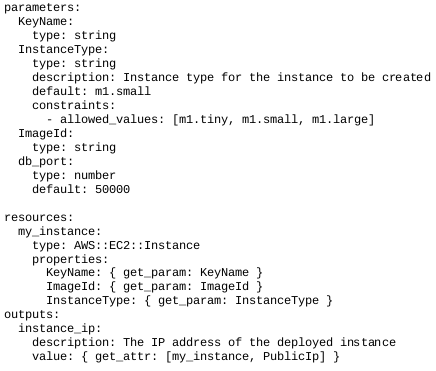
\includegraphics[width = 7cm]{exemple_parametre.png}
\caption{Exemple de paramêtre dans Heat}
\end{figure}
\subsection{Trove}
Un service de base de donnée. Sa fait un accès à une base de donné par appel de procédure à distance (RPC). Sa fait la création et la gestion de base de données. Sa nous donne accès. Sa gère les backups. sa supporte différentes bases de données relationnelles ounon (MySQL, PostgreSQL..). 
\subsection{Marconi}
Queues de messages, publication abonnement, notification. AMPQ. C'est bon pour un très grand nombres d'usagers..
\subsection{Savannah}
Service Hadoop, Semblable à Amazon Elastic map-reduce. Sa réutilisation les autres services de OpenStack. C'est commandé par Horizon, sa fait des images avec hadoop dans glance. sa prend des noeuds de calculs avec nova. Le stockage se fait sur Swift et finalement l'authentification sur fait avec Keystone.

\subsection{Discussion}
Beaucoup de grand joueurs sont impliqués. C'est une infrastructure cloud entièrement open source qui offre des fonctionnalités vraiment semblable à Amazon. Le progrès est très rapide avec de grande différences d'années à l'autre. l'essentiel de la fonctionnalité requise est maintenant disponible.\\

Le mot clé de l'heure: Infonuagique avec Software, Platform, infrastructre as a service (SaaS, PaaS, IaaS). Il n'est pas efficace d'avoir d'innombrable grappes de petites tailles.. c'est comme si tout le monde produisait son électricité, eau, viande.. Les instance virtuelles offrent toute la flexibilité à très faible couts. Par contre, il faut quand même faire attention à sa facure et au responsabilités légales.

\chapter{Top 500 + Architecture}
Les chinois sont rendus au top, c'est une source de fierté nationale. Ils n'hésitent pas sur les moyens. Pour les comparés, ont a un benchmarks assez simple, c'est genre une grande boucle. relativement facile a optimiser et représentent bien le potentiel de performance. Dans un contexte comme sa, on montre la puissance brute mais on ne montre pas la performance à résoudre un vraie problème:\\

Les tops sont rendu au alentours de 100k Teraflops (93 petaflops). Le processeur sur cet ordinateur fais environ 20GFlops. À priori, ce processeur contient environ 10 Millions de coeurs. en assumant un résultats par cycles, on peut faire le calcule.. environ 1.4 Gigaflops par processeur, fois 10 millions = environs 14 Petaflops, le reste de la performance provient du vecteur. Ils ont leur propre systèmes d'exploitation basé sur Linux ainsi que leur propre système Réseaux Sunway qui ressemble grandement à infini-band.\\

Le deuxième plus rapide (Tianhe-2) est fait de 16000 noeuds avec 2 Xeon 8 coeurs et 3 Xeon 60 coeurs chaqu'un. Sa donne un total de 3120000 coeurs au total. Utilise un Réseau TH Express-2 et produit une performance d'environ 33882 Tera Flops. Utilise Kylin Linux avec un compilateur icc.\\

Le troisième, Titan, Oak Ridge national lab, avec un système Cray avec 18688 Opterons 2,2 Ghx à 16 coeur qui donne 299008 coeurs. Ils sont monté avec des Nvidia K20X, qui donne une persomance finale de 17590 TeraFlops. Ils utilisent un Réseaux Gemini, réseuax optimiser pour ce genre de système. \\

Payer pour le réseaux dépend beaucoup du genre de problème qu'on essait d'accomplir, comme par exemple, des simulations MonteCarlo sont pas mal tous indépendant les uns des autres et ne requiert pas vraiment beaucoup d'échange entre les différents noeuds, dans ce cas, une bonne technologie réseaux n'est pas nécessairemnet utile.\\

Les ordinateurs cray était monté en cercle pour avoir une topologie régulière dans la connection des différents noeuds dans le cluster.\\

Le prochain, Sequoia, contient la technologie BlueGene d'IBM. Il contient 98304 Power BQC 1.6Ghz à 16 coeurs: ce qui donne 1572874 coeurs. Il contient un réseaux sur mesure, roule linux et produit une puissance d'environ 16328 Tera Flops. Autrefois, toutes les top contenait la technologie BlueGene.\\

Le prochain, RIKEN, contient 88124 SPARC64 VIIIfx 2.0Ghz à 8 coeurs. sa donne 705024 coeurs. Ils ont leur propre réseau TOFU (lol), roule Linux et produit environ 10510 TeraFlops\\

Mira, Juqueen, pleins d'autre roule blue gene et ont une perforance allant de 0 - 10k teraflops.\\

\section{Discussion}
Fait intéressant, nouvelle entrée dans le top 10, on à la Gyoukou, qui contient 20 millions de coeur allant à 700Mhz. Ils ont la même philosophie que le Sunway Taihulight, qui est d'avoir pleins de petits processeur efficaces et les mettres en parallèle. Chaque processeur contient environ 2048 coeurs. Leur système de refroidissement est fait à partir d'un liquide isolant, ils sont capable d'avoir une super bonne densité.\\

Ont peut voir plusieurs tendances, la compatibilité intel est une issue. Par contre, ultimement les performances ultime ne viennent pas des processeur standard. Il n'y a rien qui prouve que les processeurs intel sont meilleur que les autres (ou pire) dans ces systèmes. Maintenant on utilise des GPU/coprocesseur pour faire le gros de la programmation. En terme de puissance brute, c'est génial. Par contre, pour des utilisation un peu plus conventionnel, c'est beuacoup plus facile d'utiliser des proceseur ordinaire que des processeurs de ce style.\\

Aujourd'hui les gens ne regardent pas juste les teraflops, mais aussi les teraflops par watt.\\

Tilera avait une philosophie de faire plus de coeurs par nodes et de réduire la performance. Par contre, ils sont en faillite...\\

après la faillite de Tilera, Adapteva s'est mis dans le même mindset malgré leur équipq très petite.\\


\chapter{Exemple d'examen finaux}
\section{Examen 2016}
\subsection{Question 1a}
Ils nous demandent un programme en C qui corresponderait au programme en assembleur. On donne déjà des noms symbolique au lieu d'addresse.. alors c'est bien. On commence par charger des vecteurs. Petit bug avec VLR et 64?? C'est pas mal striaght forward, la forme SGEV.D -> $\geq$.. bref c'est sa.\\

Pour ce qui concerne le loop, mettons qu'on a 70 éléments, on va faire un and avec 63, ce que sa nous donne c'est qu'on prend seulement les bits qui sont plus petites que 63. en shiftant vers la droite pour le nombre de zéro, on se retrouve à diviser par 2 exposant le nombre de bits. ce qui nous donne R5 = 6 et R6 = 1. le premier tour de boucle va se faire seulement pour 6 éléments... Quand on parle d'uniter regrouper, c'est en fonction des opérations, comme par exemple addition et soustractions sont regrouper ensemble, il y a une uniter de multiplication et un unité de division de plus qu'une uniter de load ou de store. on peut chaîner quand les instructions se trouve dans des unités différents et en ne jouant pas sur les même registres.

\subsection{Question 1b}

La vitesse dépend du chaînage de nos instructions vectoriel. Si deux instruction consécutive sont dans des unités différentes on peut chaîner les événement (enlever le 64). Quand on commence, les chargements et rangement prennent 12 et utilise la meme unité apres alors le premier ne peut pas être chainer. par contre, le deuxieme peux le chainer. 

\subsection{1c}
Un point = un petit paragraphe. 

\subsection{2a}
\textbf{un secret, programmation opencl et MPI.}  
On cherche à faire les opérations d'addition et de soustraction de manière local, et seulement un worker du workgroup (le master) fait le transposition du résultats dans le global. on utilise la barrière pour s'assurer que tous les worker on fini les calculs avant de les transposé.

le résultats de s est (n * (n-1)/2)
\subsection{2b}
Les accès vs la cache sont le principale facteur d'impact sur la performance.  ont cherche que les work items ont des cases consecutive en memoire. on peut voir que le global id (0) varie le plus vite. \\

on cherche à maximiser la grosseur des work items pour minimiser le overhead par contre on cherche aussi à maximiser l'utilisation de notre carte graphique.\\

on multiplie le nombre de coeur SIMD par le nombre de threads (8?)
\subsection{2c}
\subsection{3a}
La boucle trie chaque zone, le reduce a comme entrer un int (le min de chaque zone) et utilise la fonction min pour avoir le min de toute les noeuds.
\subsection{3b}
all to all i1 vers i2, on modifie, all to all vers i1, voir notes (INSÉRÉ NOTES)

\subsection{3c}
MPI\_Send est bloquant. on attent qu'on à recu avant de continuer, c'est pas très performance mais sa peut nous éviter toute sorte de probleme. Bsend est bloquand aussi, sauf qu'on sauve une copie en buffer alors on peut tout de suite faire autre chose. I\_send envoie quand il peut, c'est pas nécessairement synchroniser sur rien du tout.

\subsection{4a}
on commence par faire les feuilles (D et E), étant donné qu'ils n'appellent personne. Par contre, on peut imputer ces valeurs à C et B. self + childs  = self + les imputations des différentes valeurs.

\includepdf[pages=-]{finalA2016C.pdf}
\section{Années 2014}
Le final de l'année 2014
\includepdf[pages=-]{finalA2014C.pdf}
\section{Année 2013}
Le finale de l'année 2013
\includepdf[pages=-]{finalA2013C.pdf}
\section{Année 2012}
Le final de l'année 2012
\includepdf[pages=-]{finalA2012C.pdf}

\end{document}
